\documentclass[12pt, oneside]{book}

%\usepackage[parfill]{parskip}
\usepackage{acronym, graphicx, placeins, subfig, color, tabu, todonotes, subcaption, amssymb, amsmath, amscd, fullpage, epstopdf, appendix, hyperref, setspace, tensor, url, verbatim}
\usepackage[inline]{enumitem}
%\numberwithin{equation}{section}

\hypersetup{colorlinks, citecolor = black, filecolor = black, linkcolor = black, urlcolor = black, linktocpage}

\onehalfspacing

\newcommand{\be}{\begin{equation}}
\newcommand{\ee}{\end{equation}}
\newcommand{\adag}{a^{\dag}}
\newcommand{\bra}[1]{\langle #1 \vert}
\newcommand{\ket}[1]{\vert #1\rangle}
\newcommand{\braket}[2]{\langle #1\vert #2\rangle}
\newcommand{\sminus}{\sigma_-}
\newcommand{\splus}{\sigma_+}

\DeclareMathOperator{\tr}{tr}
\newcommand{\evalue}[1]{\left\langle #1 \right\rangle}
\newcommand{\comm}[2]{\left[ #1, \, #2 \right]}
\newcommand{\modsq}[1]{\left\lvert #1 \right\rvert^2}
\newcommand{\REC}{\text{REC}}
\newcommand{\es}{\emptyset}
\newcommand{\recA}{\{ A \}}
\newcommand{\recB}{\{ B \}}
\newcommand{\recCTp}{\{ C_{T'} \}}
\newcommand{\recD}{\{ D \}}
\newcommand{\recETp}{\{ E_{T'} \}}
\newcommand{\sL}{\mathcal{L}}
\newcommand{\ZPF}{\text{ZPF}}
\newcommand{\bdag}{b^{\dag}}

\begin{document}
\thispagestyle{empty}
\singlespacing

\begin{center}
    ABSTRACT\\
    \vspace{2.0cm}
    Lightmap Generation and Parameterization\\
    \vspace{1.0cm}
    by Meisam Amjad\\
    \vspace{1.0cm}
\end{center}

\noindent Work to date in cavity optomechanics has focused primarily on the coupling between the cavity field and the mechanical oscillator. We investigate a weakly driven, damped optomechanical cavity containing a two-level atom with an oscillating end mirror or an intracavity dielectric membrane. We carry out numerical simulations of the system using the framework of quantum trajectories, implemented with the Quantum Toolbox in Python (QuTiP). We calculate the cavity probe spectrum and various second-order correlations, finding they are modified by the coupling between the cavity field and the mechanical oscillator.

\newpage

\thispagestyle{empty}

\frontmatter

\onehalfspacing

\begin{titlepage}
\begin{center}
PROBE SPECTRA AND PHOTON STATISTICS IN A \\ WEAKLY-DRIVEN CAVITY OPTOMECHANICAL SYSTEM

\vspace{1.5cm}

A Thesis \\

\vspace{0.5cm}

Submitted to the \\
Faculty of Miami University \\
in partial fulfillment of \\
the requirements for the degree of \\
Master of Science \\
Department of Physics \\
by \\
Andrew Jacobs \\
Miami University \\
Oxford, Ohio \\
2012

\vspace{1.5cm}

\emph{Advisor}: \rule[-0.1cm]{8cm}{0.01cm} \\
(James Clemens) \\
\vspace{1.5cm}
\emph{Reader}: \rule[-0.1cm]{8cm}{0.01cm} \\
(Perry Rice) \\
\vspace{1.5cm}
\emph{Reader}: \rule[-0.1cm]{8cm}{0.01cm} \\
(Samir Bali) \\
\end{center}
\end{titlepage}

\if@xetex
	\cleardoublepage
	\phantomsection
\else
	\ifpdf
		\cleardoublepage
		\phantomsection
	\else
		\cleardoublepage
	\fi
\fi

\setcounter{page}{2}
\tableofcontents
\setcounter{tocdepth}{2}
\listoffigures

\newpage

\begin{center} ACKNOWLEDGEMENTS \end{center}

\noindent I would first like to thank my advisor, Dr. James Clemens, for presenting me with this interesting problem full of rich detail, and for many conversations providing critical guidance throughout the project. I also thank him for helping me to grow as an overall student of physics, during both my time as an undergraduate and graduate student. I also thank Drs. Perry Rice and Samir Bali, for taking the time to read this thesis and offer their insights, as well as for a great deal of friendly conversation and enjoyable classroom instruction during my time in Oxford. There are countless other faculty members who deserve similar accolades, but the list is too lengthy to be shown here in completion. Last, but certainly not least, I offer a great deal of thanks to my friends and family (again, a list too lengthy to present in this space), without whom I would have lacked crucial support and guidance in maintaining my interest and desire to finish this graduate program.

\mainmatter

\chapter{Introduction}
With the advent of quantum mechanics in the early twentieth has come a slew of related fields in physics, one being quantum optics. Research in quantum optics concerns itself with a quantum mechanical treatment of the interaction between light and matter. A typical introduction to the field considers the fundamental dynamics of a single atom of two energy states interacting with a single mode of the electromagnetic field. Quantum optical principles can also be brought to bear in the manipulation of light and matter, as in an optical lattice \cite{optlattice} or atom cooling and trapping \cite{cooltrap}. Just as importantly, it is possible to generate light of a nonclassical nature, as in the case of photon antibunching \cite{quantopt}. Quantum optics has also proven invaluable in the fields of metrology and sensing \cite{sensing}, as well as in the development of quantum computation \cite{quantcompinfo}.

In this thesis, we narrow our focus to the area of cavity quantum electrodynamics (cQED), the study of which considers the interaction of one or more atoms and the electromagnetic field mode of a high-finesse optical cavity. Such studies provide an opportunity to investigate the effect of not only spontaneous emission, but stimulated emission and absorption by the atom as well. Theoretical work in this direction was pioneered by Einstein who, through statistical analysis, showed a modification of the spontaneous emission rate inside a cavity \cite{einstein1917}. The formalism of atom-field interactions was derived by Edwin Jaynes and Fred Cummings in 1963 \cite{charliethesis}. In addition, the phenomenon of squeezed light was first demonstrated in 1985 at Bell Labs \cite{charliethesis}. In squeezed light, the field is placed in a minimum uncertainty condition; unlike a coherent state, the uncertainty is unevenly distributed between field quadratures. Cavity QED has also allowed for the probing of entangled states of light and matter \cite{charliethesis}.

It is worth pausing to briefly discuss the relevance of quantum computing. Certain processes, such as Shor's algorithm, have been calculated to be much faster if carried out on a quantum computer, which could prove useful in areas such as modern cryptography. The latter allows for the factoring of very large integers, the fundamental operation used in standard RSA and other similar classical encryption schemes. Shor described how his algorithm could, when performed on a quantum computer as opposed to a classical one, be carried out in polynomial time \cite{shor1999}. The key feature of a quantum computer is its omission of classical bits in favor of quantum bits (denoted \emph{qubits}), which are able to take on not only the individual states $\ket{0}$ and $\ket{1}$, but any linear superposition of the two states. Groups researching quantum computation are primarily concerned with the measurement and interaction of qubits. Quantum algorithms take advantage of entanglement between qubits, which requires strong correlations. Various dissipative processes will destroy such correlation, and cQED presents an opportunity to modify such dissipation \cite{charliethesis}.

In this thesis, we add an additional element to the standard cQED model--a mechanical oscillator. The study of this field is known as cavity optomechanics (cOM), and presents another degree of freedom for controlling and modifying the dissipative processes within the cavity. We compare various attributes of the atom and field mode to the expected results of standard cQED, as well as calculating relevant quantities for the mechanical oscillator.

\section{Optomechanical Model}
Many variations of cOM are possible, and we mention a few before specializing to our particular scenario. Perhaps the best survey of cOM configurations comes from Kippenberg and Vahala \cite{kippenberg2007}, who first illustrate the canonical optomechanical apparatus: a pair of mirrors, one of which is harmonically bound by a mechanical spring. The authors then cite a list of experimental realizations that includes cantilevers \cite{kleckner2006}, micro-mirrors \cite{arcizet2006, gigan2006}, toroidal micro-cavities \cite{kippenberg2005, schliesser2006}, nano-membranes \cite{thompson2007}, and macroscopic mirror modes \cite{corbitt2007}.

We begin by describing the standard cQED model, and then append the relevant optomechanical features. A single two-level atom, with respective ground and excited energy states $\ket{g}$ and $\ket{e}$, is placed in the optical cavity, whose field mode is weakly driven at a rate $Y$; the atom and cavity mode interact at the coupling rate $g$. We then expect an oscillation of the atom between its two energy states at an identical rate $g$; this may be generalized to a rate $g\sqrt{n}$ for $n$ photons \cite{phasespace}.

However, there is also the issue of dissipation in the system. The system can leak photons in one of two ways: (i) spontaneous emission from the atom, and (ii) cavity field mode leakage from one of the end mirrors. The first phenomenon occurs when the atom absorbs a photon from the driving field and subsequently re-emits in a random direction; this takes place at a rate $\gamma$ that is analogous to the Einstein $A$ coefficient; note the two are only identical in the free space limit. Emission from the cavity mode occurs at a rate $2\kappa$, where $\kappa = cT_m/2L$. The transmission probability of the mirror is denoted $T_m$, $L$ is the length of the cavity, and $c$ is the speed of light \cite{charliethesis}.

This is the driven Jaynes-Cummings model of cQED including dissipative losses. We now introduce the mechanical oscillator to the system, represented by a physical spring coupling one of the end mirrors to a static surface. The resonance frequency of the spring is denoted $\omega_M$, while $M$ is the mass of the mirror; we define $x$ to be the mirror's distance from its equilibrium position, and will later write this in terms of quantum mechanical operators. The cavity mode and oscillator interact at a rate $g_M$, and an additional degree of dissipation may be included by a phonon decay rate in the spring of $\kappa_M$. We discuss these parameters in greater detail later in the thesis; below is an illustration \cite{kippenberg2007} of our imagined cOM apparatus and the important rates.

\begin{figure}[htb]
\begin{center}
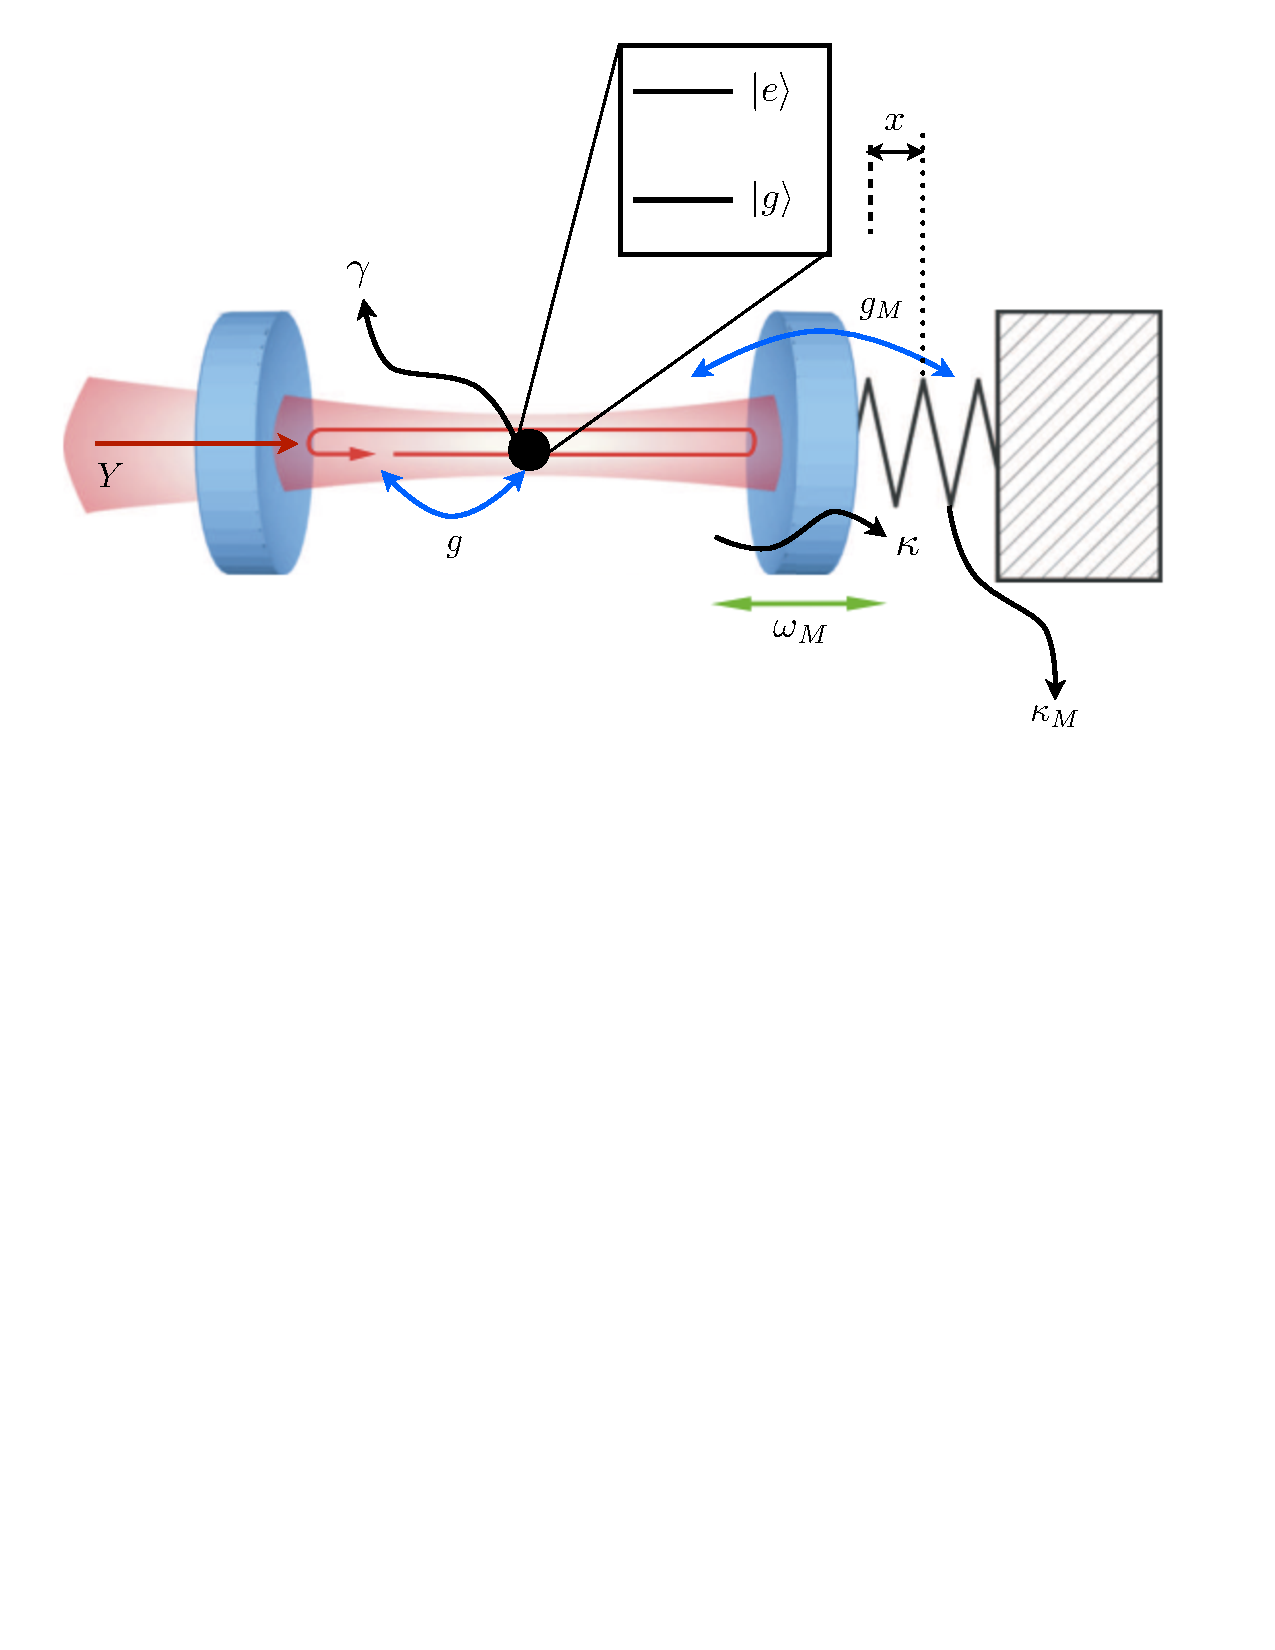
\includegraphics[width=0.7\textwidth]{Figures/1Apparatus}
\caption[A schematic of our imagined cavity optomechanics apparatus]{\small{A schematic of our imagined cavity optomechanics apparatus. The driving rate $Y$ is shown in red, while dissipative losses are drawn in black and coupling rates are blue. We also show the displacement of the oscillator, and length $L$ is the distance between the two end mirrors, which will oscillate in time.}}
\label{fig1Apparatus}
\end{center}
\end{figure}

We consider the apparatus of Fig.~\ref{fig1Apparatus} by starting with an optomechanical, non-Hermitian Hamiltonian demonstrating coupling between the cavity and oscillator that goes linearly with displacement. The method of quantum trajectory theory is implemented using the Quantum Toolbox in Python, or QuTiP \cite{qutipref}. The software is able to numerically calculate the state of the system and any stated expectation values over a range of times. With only slight adjustment, we can also calculate probe spectra and second-order correlation values. We plot various quantities and compare the results to what is expected from the Jaynes-Cummings cQED model. Ultimately, we aim to determine modifications due to the introduction of the mechanical oscillator.

\section{Outline of Thesis}
In chapter two, we detail the three primary theoretical frameworks used in this thesis. First, we derive the master equation in standard Lindblad form, detailing the various approximations made to achieve the form used. Second, we follow the approach of Carmichael and illustrate quantum trajectory theory, as well as explaining its advantage in QuTiP over the differential equation solver as applied to the Schr\"{o}dinger equation. Lastly, we explicitly write the Hamiltonian for the atom-field-oscillator system and detail the various parameters assigned to the mechanical spring. In chapter three, we treat the oscillator as a classical object, considering its dynamics when modeled as a harmonic oscillator and then when placed in a thermal state. Chapter four brings us to a fully quantum mechanical realization, and we determine probe spectra along with atom-field and field-field second-order correlations $g^{(2)}(0)$ and $g^{(2)}(\tau)$. Finally, in chapter five we summarize our results and point to future work for a weakly-driven optomechanical cavity with a two-level atom.
\chapter{Theoretical Frameworks}
With this portion of the thesis, we introduce three essential aspects of the theoretical background of our approach to cavity optomechanics. First, we start with the Schr\"{o}dinger equation and, using the system-plus-reservoir approach detailed by Carmichael in \cite{howard1}, invoke the Born-Markov approximation to derive the master equation in standard Lindblad form, a necessary result for open quantum systems. Second, we again follow the approach of Carmichael in \cite{howard2} to describe the theory of quantum trajectories, a crucial technique for following the time evolution of a quantum system, in this case the optomechanical cavity. Lastly, we describe the basic approach in our choice of Hamiltonian and parameters of note in the cOM apparatus.

\section{Derivation of the Master Equation}
We begin by writing a Hamiltonian of three terms,
%
\be H = H_S + H_R + H_{SR}, \label{eq2.1} \ee
%
describing the respective dynamics of the system, the reservoir, and their interaction \cite{howard1}. The full density operator describing both the system and reservoir is denoted $\chi(t)$, and taking the partial trace over the reservoir yields
%
\be \rho(t) = \tr_R \chi(t), \label{eq2.2} \ee
%
the density operator describing only the system. Note that, in general, the expectation value for some observable $\hat{O}$ of the system can be calculated using the density operator by
%
\[ \evalue{\hat{O}} = \tr_{SR} \left( \hat{O} \chi \right) = \tr_S \left( \hat{O} \, \tr_R \chi \right) = \tr_S \left( \hat{O} \rho \right). \]
%
In the second equality, we have pulled the operator $\hat{O}$ through the partial trace over the reservoir as it is only affected by system dynamics, while the final equality reflects \eqref{eq2.2}. Note that, for the time being, we suppress writing any time dependence. We write the equation of motion for the full density operator as
%
\be \dot{\chi} = -\frac{i}{\hbar} \comm{H}{\chi}, \label{eq2.3} \ee
%
where $H$ is the full Hamiltonian of \eqref{eq2.1}. This can be validated by first expanding the density operator as a sum over state vectors,
%
\be \chi = \sum_{\ket{\psi}} P_{\ket{\psi}} \, \ket{\psi} \bra{\psi}, \label{eq2.4} \ee
%
where $P_{\ket{\psi}}$ is the probability for a given state vector. We then calculate the explicit form of the left-hand side of \eqref{eq2.3},
%
\be \dot{\chi} = \sum_{\ket{\psi}} P_{\ket{\psi}} \left( \ket{\psi} \bra{\dot{\psi}} + \ket{\dot{\psi}} \bra{\psi} \right). \label{eq2.5} \ee
%
Using the Schr\"{o}dinger equation,
%
\[ \ket{\dot{\psi}} = -\frac{i}{\hbar} H \ket{\psi}, \quad \bra{\dot{\psi}} = \bra{\psi} H \left( \frac{i}{\hbar} \right), \]
%
we may rewrite \eqref{eq2.5} as
%
\be \dot{\chi} = -\frac{i}{\hbar} H\chi + \frac{i}{\hbar} \chi H, \label{eq2.6} \ee
%
verifying \eqref{eq2.3}. Transforming to the interaction picture, we define a modified composite density operator,
%
\be \tilde{\chi} = e^{i(H_S + H_R)t/\hbar} \, \chi \, e^{-i(H_S + H_R)t/\hbar}. \label{eq2.7} \ee
%
Taking the time derivative of \eqref{eq2.7} we find,
%
\be \dot{\tilde{\chi}} = e^{\alpha t} \, \chi \left( -\alpha \right) e^{-\alpha t} + e^{\alpha t} \, \dot{\chi} \, e^{-\alpha t} + \alpha \, e^{\alpha t} \, \chi \, e^{-\alpha t}, \label{eq2.8} \ee
%
where we have defined
%
\be \alpha \equiv \frac{i}{\hbar} \left( H_S + H_R \right). \label{eq2.9} \ee
%
Using the relations \eqref{eq2.6} and \eqref{eq2.7}, as well as the fact that $H_S$ and $H_R$ commute both with themselves and each other, we rewrite \eqref{eq2.8} as
%
\[ \dot{\tilde{\chi}} = -\frac{i}{\hbar} \tilde{\chi} \left( H_S + H_R \right) + \alpha \tilde{\chi} - \frac{i}{\hbar} e^{\alpha t} \comm{H}{\chi} e^{-\alpha t}, \]
%
or
%
\be \dot{\tilde{\chi}} = \frac{i}{\hbar} \comm{H_S + H_R}{\tilde{\chi}} - \frac{i}{\hbar} e^{\alpha t} \comm{H_S + H_R + H_{SR}}{\chi} e^{-\alpha t}. \label{eq2.10} \ee
%
We pause to note that without the interaction Hamiltonian $H_{SR}$, the modified composite density operator $\tilde{\chi}$ becomes static in time. Returning to \eqref{eq2.10}, if we split up the second commutator such that $H_{SR}$ stands alone, the equation of motion for $\tilde{\chi}$ simplifies greatly to
%
\be \dot{\tilde{\chi}} = -\frac{i}{\hbar} e^{\alpha t} \comm{H_{SR}}{\chi} e^{-\alpha t}. \label{eq2.11} \ee
%
We cleverly choose to rewrite the commutator as
%
\[ \comm{H_{SR}}{\chi} \to H_{SR} \left( e^{-\alpha t} e^{\alpha t} \right) \chi - \chi \left( e^{-\alpha t} e^{\alpha t} \right) H_{SR}, \]
%
such that \eqref{eq2.11} becomes
%
\be \dot{\tilde{\chi}} = -\frac{i}{\hbar} \comm{\tilde{H}_{SR}}{\tilde{\chi}}, \label{eq2.12} \ee
%
where we have defined
%
\be \tilde{H}_{SR} \equiv e^{\alpha t} \, H_{SR} \, e^{-\alpha t}. \label{eq2.13} \ee
%
We now have an equation of motion where both the density operator and Hamiltonian are written in the interaction picture. This defines a valid scheme for damping in the system due to coupling with some type of thermal reservoir. This form represents a substantial simplification because, after two transformations, one each to $H_{SR}$ and $\chi$, the individual system and reservoir Hamiltonians have vanished. In this treatment, they are considered a baseline that is subtracted away, allowing us to focus strictly on the interaction terms.

Ultimately, we are looking to obtain an equation of motion, a master equation, for the reduced density operator $\rho(t)$ of \eqref{eq2.2} reflecting the dynamics of the system. In our approach, as per \cite{howard1}, we continue by integrating \eqref{eq2.12} with respect to time,
%
\be \int_0^t \frac{d}{dt'} (\tilde{\chi}) \, dt' = -\frac{i}{\hbar} \int_0^t \comm{\tilde{H}_{SR}(t')}{\tilde{\chi}(t')} dt', \label{eq2.14} \ee
%
where we have reintroduced the time dependence of the various operators. This simplifies to
%
\be \tilde{\chi}(t) = \tilde{\chi}(0) - \frac{i}{\hbar} \int_0^t \comm{\tilde{H}_{SR}(t')}{\tilde{\chi}(t')} dt', \label{eq2.15} \ee
%
and substituting \eqref{eq2.15} into \eqref{eq2.12} yields
%
\begin{align} \dot{\tilde{\chi}}(t) &= -\frac{i}{\hbar} \comm{\tilde{H}_{SR}(t)}{\left\{ \tilde{\chi}(0) - \frac{i}{\hbar} \int_0^t \comm{\tilde{H}_{SR}(t')}{\tilde{\chi}(t')} dt' \right\}} \nonumber \\
&= -\frac{i}{\hbar} \comm{\tilde{H}_{SR}(t)}{\tilde{\chi}(0)} - \frac{1}{\hbar^2} \int_0^t \comm{\tilde{H}_{SR}(t)}{\comm{\tilde{H}_{SR}(t')}{\tilde{\chi}(t')}} dt'. \label{eq2.16} \end{align}
%
We now make our first approximation, which is that for time $t = 0$, the system $S$ and reservoir $R$ factorize; in other words, the system and reservoir are initially noninteracting. This allows us to write the composite density operator as the product of density operators describing the system and reservoir individually,
%
\be \chi(0) = \rho(0) \, R_0. \label{eq2.17} \ee
%
Keeping this condition in mind, we consider the partial trace $\tr_R \tilde{\chi}(t)$; based on \eqref{eq2.2} we might infer that $\tr_R \tilde{\chi}(t) = \tilde{\rho}(t)$, but it would be wise to show this formally. Using the explicit form of the modified composite density operator, the partial trace is
%
\be \tr_R \tilde{\chi}(t) = \tr_R \left[ e^{\alpha t} \, \chi(t) \, e^{-\alpha t} \right]. \label{eq2.18} \ee
%
Separating system and reservoir terms using \eqref{eq2.9}, the latter partial trace becomes
%
\begin{align} \tr_R \tilde{\chi}(t) &= \tr_R \left[ e^{iH_S t/\hbar} \, e^{iH_R t/\hbar} \, \chi(t) \, e^{-iH_R t/\hbar} \, e^{-iH_S t/\hbar} \right] \nonumber \\
&= e^{iH_S t/\hbar} \, \tr_R \left[ e^{iH_R t/\hbar} \, \chi(t) \, e^{-iH_R t/\hbar} \right] e^{-iH_S t/\hbar}, \label{eq2.19} \end{align}
%
where we have pulled system terms through the partial trace over the reservoir. Using the cyclic property of the trace, the reservoir exponentials cancel in \eqref{eq2.19}, and based on \eqref{eq2.2} we find that
%
\be \tr_R \tilde{\chi}(t) = e^{iH_S t/\hbar} \, \rho(t) \, e^{-iH_S t/\hbar} = \tilde{\rho}(t). \label{eq2.20} \ee
%
This verifies our earlier inference. Considering \eqref{eq2.16}, \eqref{eq2.17}, and \eqref{eq2.20}, we can now write the partial trace over the reservoir of the equation of motion for $\tilde{\chi}$,
%
\be \begin{split} \tr_R \dot{\tilde{\chi}}(t) &= -\frac{i}{\hbar} \, \tr_R \left\{ \comm{\tilde{H}_{SR}(t)}{\tilde{\rho}(0) \, \tilde{R}_0} \right\} \\ &\qquad - \frac{1}{\hbar^2} \int_0^t \tr_R \left\{ \comm{\tilde{H}_{SR}(t)}{\comm{\tilde{H}_{SR}(t')}{\tilde{\chi}(t')}} \right\} dt', \label{eq2.21} \end{split} \ee
%
which simplifies to
%
\be \dot{\tilde{\rho}} = -\frac{1}{\hbar^2} \int_0^t \tr_R \left\{ \comm{\tilde{H}_{SR}(t)}{\comm{\tilde{H}_{SR}(t')}{\tilde{\chi}(t')}} \right\} dt'. \label{eq2.22} \ee
%
The first term in \eqref{eq2.21} vanishes on the assumption that any reservoir operators have zero mean in $R_0$. If this is not already the case, it can be arranged by including a term $\tr_R(H_{SR} R_0)$ in the system Hamiltonian $H_S$. We now have a differential equation in $\tilde{\rho}$ via \eqref{eq2.22}.

A second approximation is now introduced, which states that system and reservoir correlations arise at order $H_{SR}$, and are assumed to be small. Physically, this means the system only weakly affects the reservoir due to the large size of the latter. We write
%
\be \tilde{\chi}(t) = \tilde{\rho}(t) \, R_0 + O(H_{SR}), \label{eq2.23} \ee
%
where $R_0$ is stationary. This approximation is indicative of time-dependent perturbation theory, and we keep only terms to second order in $H_{SR}$. We rewrite \eqref{eq2.22} as
%
\be \dot{\tilde{\rho}}(t) = -\frac{1}{\hbar^2} \int_0^t \tr_R \left\{ \comm{\tilde{H}_{SR}(t)}{\comm{\tilde{H}_{SR}(t')}{\tilde{\rho}(t') \, R_0}} \right\} dt'. \label{eq2.24} \ee
%
The condition represented by \eqref{eq2.23} is known as the Born approximation. It leads logically to the second approximation essential to our approach, where we simplify the reduced density operator as
%
\be \tilde{\rho}(t') \to \tilde{\rho}(t), \label{eq2.25} \ee
%
which indicates the system has ``no memory.'' Physically, this indicates that energy will leak out of the system into the reservoir and not return; the time evolution of the system depends only upon its present state and is unaffected by past conditions. We have defined the Markov approximation, and as such \eqref{eq2.23} and \eqref{eq2.25} collectively represent the Born-Markov approximation. Equation~\eqref{eq2.24} can now be written as
%
\be \dot{\tilde{\rho}}(t) = -\frac{1}{\hbar^2} \int_0^t \tr_R \left\{ \comm{\tilde{H}_{SR}(t)}{\comm{\tilde{H}_{SR}(t')}{\tilde{\rho}(t) \, R_0}} \right\} dt'. \label{eq2.26} \ee
%
It is important that we pause at this point to justify the use of the Markov approximation. In order to do so, we recast the interaction Hamiltonian as a sum of products of system ($s_i$) and reservoir ($\Gamma_i$) operators,
%
\be H_{SR} = \hbar \sum_i s_i(t) \, \Gamma_i(t). \label{eq2.27} \ee
%
In the interaction picture, the Hamiltonian becomes
%
\begin{align} \tilde{H}_{SR} &= \hbar \sum_i e^{\alpha t} \, s_i(t) \, \Gamma_i(t) \, e^{-\alpha t} \nonumber \\
&= \hbar \sum_i \left[ e^{iH_S t/\hbar} \, s_i(t) \, e^{-iH_S t/\hbar} \right] \left[ e^{iH_R t/\hbar} \, \Gamma_i(t) \, e^{-iH_R t/\hbar} \right] \nonumber \\
&= \hbar \sum_i \tilde{s}_i(t) \, \tilde{\Gamma}_i(t). \label{eq2.28} \end{align}
%
Invoking only the Born approximation at this time, substituting \eqref{eq2.28} into \eqref{eq2.24} yields
%
\be \dot{\tilde{\rho}}(t) = -\sum_{i,j} \int_0^t \tr_R \left\{ \comm{\tilde{s}_i(t) \, \tilde{\Gamma}_i(t)}{\comm{\tilde{s}_j(t') \, \tilde{\Gamma}_j(t')}{\tilde{\rho}(t') \, R_0}} \right\} dt', \label{eq2.29} \ee
%
where the double sum is a result of the different times at which the operators are considered ($t$ versus $t'$). We expand \eqref{eq2.29} as
%
\be \begin{split} \dot{\tilde{\rho}}(t) &= -\sum_{i,j} \int_0^t \tr_R \left\{ \tilde{s}_i(t) \, \tilde{\Gamma}_i(t) \comm{\tilde{s}_j(t') \, \tilde{\Gamma}_j(t')}{\tilde{\rho}(t') \, R_0} \right. \\
&\qquad \left. - \comm{\tilde{s}_j(t') \, \tilde{\Gamma}_j(t')}{\tilde{\rho}(t') \, R_0} \tilde{s}_i(t) \, \tilde{\Gamma}_i(t) \right\} dt', \label{eq2.30} \end{split} \ee
%
and by expanding the remaining commutators,
%
\be \begin{split} \dot{\tilde{\rho}}(t) &= -\sum_{i,j} \int_0^t \tr_R \left\{ \tilde{s}_i(t) \, \tilde{\Gamma}_i(t) \, \tilde{s}_j(t') \, \tilde{\Gamma}_j(t') \, \tilde{\rho}(t') \, R_0 \right. \\
&\qquad - \tilde{s}_i(t) \, \tilde{\Gamma}_i(t) \, \tilde{\rho}(t') \, R_0 \, \tilde{s}_j(t') \, \tilde{\Gamma}_j(t') - \tilde{s}_j(t') \, \tilde{\Gamma}_j(t') \, \tilde{\rho}(t') \, R_0 \, \tilde{s}_i(t) \, \tilde{\Gamma}_i(t) \\
&\qquad + \left. \tilde{\rho}(t') \, R_0 \, \tilde{s}_j(t') \, \tilde{\Gamma}_j(t') \, \tilde{s}_i(t) \, \tilde{\Gamma}_i(t) \right\} dt'. \label{eq2.31} \end{split} \ee
%
By pulling any system operators, namely the $\tilde{s}_i$, $\tilde{s}_j$, and $\tilde{\rho}$, through the partial trace over the reservoir, \eqref{eq2.31} becomes slightly more compact:
%
\be \begin{split} \dot{\tilde{\rho}}(t) &= -\sum_{i,j} \int_0^t \left\{ \tilde{s}_i(t) \, \tilde{s}_j(t') \, \tilde{\rho}(t') \, \tr_R \left[ \tilde{\Gamma}_i(t) \, \tilde{\Gamma}_j(t') \, R_0 \right] \right. \\
&\qquad - \tilde{s}_i(t) \, \tilde{\rho}(t') \, \tilde{s}_j(t') \, \tr_R \left[ \tilde{\Gamma}_i(t) \, R_0 \, \tilde{\Gamma}_j(t') \right] \\
&\qquad - \tilde{s}_j(t') \, \tilde{\rho}(t') \, \tilde{s}_i(t) \, \tr_R \left[ \tilde{\Gamma}_j(t') \, R_0 \, \tilde{\Gamma}_i(t) \right] \\
&\qquad + \left. \tilde{\rho}(t') \, \tilde{s}_j(t') \, \tilde{s}_i(t) \, \tr_R \left[ R_0 \, \tilde{\Gamma}_j(t') \, \tilde{\Gamma}_i(t) \right] \right\} dt'. \label{eq2.32} \end{split} \ee
%
Using both the cyclic property of the trace and the relation $\tr_R (\hat{O} \hat{\chi}) = \langle \hat{O} \rangle$, where $\hat{\chi}$ is a generalized density matrix, we arrive at
%
\be \begin{split} \dot{\tilde{\rho}}(t) &= -\sum_{i,j} \int_0^t \left\{ \left[ \tilde{s}_i(t) \, \tilde{s}_j(t') \, \tilde{\rho}(t') - \tilde{s}_j(t') \, \tilde{\rho}(t') \, \tilde{s}_i(t) \right] \evalue{\tilde{\Gamma}_i(t) \, \tilde{\Gamma}_j(t')} \right. \\
&\qquad + \left. \left[ \tilde{\rho}(t') \, \tilde{s}_j(t') \, \tilde{s}_i(t) - \tilde{s}_i(t) \, \tilde{\rho}(t') \, \tilde{s}_j(t') \right] \evalue{\tilde{\Gamma}_j(t') \, \tilde{\Gamma}_i(t)} \right\} dt'. \label{eq2.33} \end{split} \ee
%
The Markov approximation is easily grasped from \eqref{eq2.33} if we conclude that the reservoir operators $\tilde{\Gamma}_i(t)$ and $\tilde{\Gamma}_j(t')$ are delta-correlated,
%
\be \evalue{\tilde{\Gamma}_i(t) \, \tilde{\Gamma}_j(t')} \simeq \delta(t - t'), \label{eq2.34} \ee
%
as this is only possible at $t = t'$, which matches the condition of \eqref{eq2.25}. The Markov approximation is also only valid when correlation times are small relative to the system evolution timescale. This explains why modeling the reservoir as an enormous set of thermal modes works so well; a reservoir of lasers would be highly undesirable as correlation times would grow very large.

Up to this point, we have made no specification as to the system operators. Now we choose to consider a single damped harmonic oscillator for our system, and continue to model the reservoir as a large ensemble of thermal modes. The Hamiltonians of \eqref{eq2.1} and the reservoir density operator are
%
\begin{subequations} \begin{align}
H_S &= \hbar\omega_0 \, \adag a, \label{eq2.35a} \\
H_R &= \sum_j \hbar\omega_j \, r^{\dag}_j r_j, \label{eq2.35b} \\
H_{SR} &= \hbar \sum_j \left( \kappa^{\ast}_j \, a r^{\dag}_j + \kappa_j \, \adag r_j \right) = \hbar \left( a \Gamma^{\dag} + \adag \Gamma \right), \label{eq2.35c} \\
R_0 &= \prod_j \exp \left( -\frac{\hbar\omega_j}{k_B T} \, r^{\dag}_j r_j \right) \left[ 1 - \exp \left( -\frac{\hbar\omega_j}{k_B T} \right) \right], \label{eq2.35d} \end{align} \end{subequations}
%
where the index $j$ denotes a single mode of the reservoir and we have defined a total reservoir operator $\Gamma = \sum_j \kappa_j r_j$. Matching the corresponding operators from \eqref{eq2.33} to those of \eqref{eq2.35a}-\eqref{eq2.35c} we find
%
\be s_1 = a, \quad \tilde{s}_1 = a \, e^{-i\omega_0 t}, \quad s_2 = \adag, \quad \tilde{s}_2 = \adag \, e^{i\omega_0 t}, \quad \Gamma_1 = \Gamma^{\dag}, \quad \Gamma_2 = \Gamma. \label{eq2.36} \ee
%
Having defined these correspondences, we are able to evaluate the two-time correlation functions in \eqref{eq2.33} for all combinations of $i$, $j$ = 1, 2. In no particular order these are
%
\begin{subequations} \begin{align}
\evalue{\tilde{\Gamma}^{\dag}(t) \, \tilde{\Gamma}^{\dag}(t')} &= 0, \label{eq2.37a} \\
\evalue{\tilde{\Gamma}(t) \, \tilde{\Gamma}(t')} &= 0, \label{eq2.37b} \\
\evalue{\tilde{\Gamma}^{\dag}(t) \, \tilde{\Gamma}(t')} &= \evalue{\tilde{\Gamma}^{\dag}(t) \, \tilde{\Gamma}(t - \tau)} \nonumber \\
&= \int_0^{\infty} e^{i\omega\tau} \, g(\omega) \modsq{\kappa(\omega)} \evalue{r^{\dag}_j r_j} d\omega \nonumber \\
&= \int_0^{\infty} e^{i\omega\tau} \, g(\omega) \modsq{\kappa(\omega)} \bar{n}(\omega, \, T) \, d\omega, \label{eq2.37c} \\
\evalue{\tilde{\Gamma}(t) \, \tilde{\Gamma}^{\dag}(t - \tau)} &= \int_0^{\infty} e^{-i\omega\tau} \, g(\omega) \modsq{\kappa(\omega)} \left[ \bar{n}(\omega, \, T) + 1 \right] d\omega. \label{eq2.37d} \end{align} \end{subequations}
%
Considering first \eqref{eq2.37a}, we note this correlation may be approximated by $\sum_j \langle r^{\dag}_j r^{\dag}_j \rangle$ or $\sum_{i,j} \langle r^{\dag}_i r^{\dag}_j \rangle$, which can then be factorized as $\sum_{i,j} \langle r^{\dag}_i \rangle \, \langle r^{\dag}_j \rangle$. Both of these expectation values will vanish due to the thermal fluctuations of the reservoir; an analogous argument can be made to justify \eqref{eq2.37b}. Next we see in \eqref{eq2.37c} a new time variable $\tau$ defined by $t' \equiv t - \tau$. The exponential term arises from the product $e^{-i\omega_j t} \, e^{i\omega_j (t - \tau)}$, and the Hermitian conjugate appears in \eqref{eq2.37d}. The function $g(\omega)$ denotes the density of states required to convert from a sum to an integral over frequencies, while $\modsq{\kappa(\omega)}$ indicates a Lorentzian linewidth of the mode. Finally, $\langle r^{\dag}_j r_j \rangle = \bar{n}(\omega, \, T)$ is the frequency- and temperature-dependent mean photon number. This is slightly modified in \eqref{eq2.37d} due to the commutation relation
%
\[ \evalue{r_j r^{\dag}_j} = \evalue{r^{\dag}_j r_j + \comm{r_j}{r^{\dag}_j}} = \evalue{r^{\dag}_j r_j} + 1. \]
%
Having specified the system and reservoir operators and evaluated the possible correlation functions, we substitute the operators of \eqref{eq2.36} into \eqref{eq2.33} to find
%
\be \begin{split} \dot{\tilde{\rho}}(t) &= -\int_0^t \left\{ \left[ a \, e^{-i\omega_0 t} \, \adag \, e^{i\omega_0 t'} \, \tilde{\rho}(t') - \adag \, e^{i\omega_0 t'} \, \tilde{\rho}(t') \, a \, e^{-i\omega_0 t} \right] \evalue{\tilde{\Gamma}^{\dag}(t) \, \tilde{\Gamma}(t')} \right. \\
&\qquad + \left[ \tilde{\rho}(t') \, \adag \, e^{i\omega_0 t'} \, a \, e^{-i\omega_0 t} - a \, e^{-i\omega_0 t} \, \tilde{\rho}(t') \, \adag \, e^{i\omega_0 t'} \right] \evalue{\tilde{\Gamma}(t') \, \tilde{\Gamma}^{\dag}(t)} \\
&\qquad + \left[ \adag \, e^{i\omega_0 t} \, a \, e^{-i\omega_0 t'} \, \tilde{\rho}(t') - a \, e^{-i\omega_0 t'} \, \tilde{\rho}(t') \, \adag \, e^{i\omega_0 t} \right] \evalue{\tilde{\Gamma}(t) \, \tilde{\Gamma}^{\dag}(t')} \\
&\qquad + \left. \left[ \tilde{\rho}(t') \, a \, e^{-i\omega_0 t'} \, \adag \, e^{i\omega_0 t} - \adag \, e^{i\omega_0 t} \, \tilde{\rho}(t') \, a \, e^{-i\omega_0 t'} \right] \evalue{\tilde{\Gamma}^{\dag}(t') \, \tilde{\Gamma}(t)} \right\} dt'. \label{eq2.38} \end{split} \ee
%
In order to simplify \eqref{eq2.38}, we use the definition $\tau = t - t'$ to determine the differential $d\tau = -dt'$; because this will cause both a sign cancellation and a reversal of the integral limits, we can leave the minus sign in place as well as the limits from $0 \to t$. We also employ the Markov approximation, letting $\tilde{\rho}(t') = \tilde{\rho}(t - \tau) \to \tilde{\rho}(t)$. This simplifies \eqref{eq2.38} to
%
\be \begin{split} \dot{\tilde{\rho}}(t) &= -\left[ a \, \adag \, \tilde{\rho}(t) - \adag \, \tilde{\rho}(t) \, a \right] \int_0^t e^{-i\omega_0 \tau} \evalue{\tilde{\Gamma}^{\dag}(t) \, \tilde{\Gamma}(t - \tau)} d\tau + \text{H.c.} \\
&\qquad -\left[ \adag \, a \, \tilde{\rho}(t) - a \, \tilde{\rho}(t) \, \adag \right] \int_0^t e^{i\omega_0 \tau} \evalue{\tilde{\Gamma}(t) \, \tilde{\Gamma}^{\dag}(t - \tau)} d\tau + \text{H.c.}, \label{eq2.39} \end{split} \ee
%
where H.c. refers to the Hermitian conjugate of the preceding term. There are now two double integrals to evaluate in \eqref{eq2.39} due to \eqref{eq2.37c} and \eqref{eq2.37d}, and we abbreviate these double integrals in the following way:
%
\begin{subequations} \begin{align}
I_1 &= \int_0^t e^{-i\omega_0 \tau} \, d\tau \int_0^{\infty} e^{i\omega\tau} \, g(\omega) \modsq{\kappa(\omega)} \bar{n}(\omega, \, T) \, d\omega \nonumber \\
&= \int_0^t d\tau \int_0^{\infty} e^{i(\omega - \omega_0)\tau} \, g(\omega) \modsq{\kappa(\omega)} \bar{n}(\omega, \, T) \, d\omega, \label{eq2.40a} \\
I_2 &= I_1 + \int_0^t d\tau \int_0^{\infty} e^{i(\omega_0 - \omega)\tau} \, g(\omega) \modsq{\kappa(\omega)} d\omega, \label{eq2.40b} \\
&= I_1 + I_3. \label{eq2.40c} \end{align} \end{subequations}
%
Because the $d\tau$ integrals are dominated by short timescales, i.e. only small values of $t$ contribute, we can change the limits on these integrals to $0 \to \infty$. The temporal integrals then evaluate to a delta function, which allows us to evaluate the frequency integral, yielding
%
\be I_1 = \pi \, g(\omega_0) \modsq{\kappa(\omega_0)} \bar{n}(\omega_0, \, T) + i\Delta'. \label{eq2.41} \ee
%
The last term in \eqref{eq2.41} refers to the complex portion of the integral, which arises from only evaluating the integral over the limits (0, $\infty$) rather than ($-\infty$, $+\infty$). We simplify $I_1$ further by defining a new variable $\gamma = 2\pi \, g(\omega_0) \modsq{\kappa(\omega_0)}$ such that
%
\be I_1 = \frac{\gamma}{2} \bar{n} + i\Delta', \label{eq2.42} \ee
%
and similarly
%
\be I_3 = \pi \, g(\omega_0) \modsq{\kappa(\omega_0)} + i\Delta = \frac{\gamma}{2} + i\Delta. \label{eq2.43} \ee
%
Taking the sum of the results of \eqref{eq2.42} and \eqref{eq2.43} yields
%
\be I_2 = \frac{\gamma}{2} \left( \bar{n} + 1 \right) + i \left( \Delta' + \Delta \right). \label{eq2.44} \ee
%
We point out that $\Delta'$ and $\Delta$ are, physically, energy level shifts, and it is possible to choose $H_S$ with a frequency $\omega_0$ such that these shifts disappear. Making such a choice at this time and omitting the complex term, \eqref{eq2.39} simplifies to
%
\be \begin{split} \dot{\tilde{\rho}}(t) &= -\frac{\gamma}{2} \bar{n} \left[ a\adag \, \tilde{\rho}(t) - \adag \, \tilde{\rho}(t) \, a + \tilde{\rho}(t) \, a\adag - \adag \, \tilde{\rho}(t) \, a \right] \\
&\qquad - \frac{\gamma}{2} \left( \bar{n} + 1 \right) \left[ \adag a \, \tilde{\rho}(t) - a \, \tilde{\rho}(t) \, \adag + \tilde{\rho}(t) \, \adag a - a \, \tilde{\rho}(t) \, \adag \right], \label{eq2.45} \end{split} \ee
%
or, suppressing the time dependence of the density operator,
%
\be \dot{\tilde{\rho}} = \frac{\gamma}{2} \bar{n} \left( 2\adag \tilde{\rho} a - a\adag \tilde{\rho} - \tilde{\rho} a\adag \right) + \frac{\gamma}{2} \left( \bar{n} + 1 \right) \left( 2 a \tilde{\rho} \adag - \adag a \tilde{\rho} - \tilde{\rho} \adag a \right). \label{eq2.46} \ee
%
This is the master equation in standard Lindblad form for a damped harmonic oscillator in the interaction picture. It will be abbreviated further in our consideration of cOM as we will operate in the limit $T \to 0$ such that $\bar{n} \to 0$ and
%
\be \dot{\tilde{\rho}} = \frac{\gamma}{2} \left( 2a \tilde{\rho} \adag - \adag a \tilde{\rho} - \tilde{\rho} \adag a \right). \label{eq2.47} \ee
%
We have achieved the goal of Section~2.1, and will refer to \eqref{eq2.47} in writing the full master equation of our cOM apparatus in the interaction picture later in Chapter~2.

\section{Quantum Trajectories}
In considering a cQED experiment, there are effectively an infinite number of variables to consider if we measure the inputs and outputs of the system and all possible reservoir modes. Quantum trajectory theory seeks to remedy this impasse by modeling cQED as a scattering experiment \cite{howard2}.
%
\begin{figure}[htb]
\begin{center}
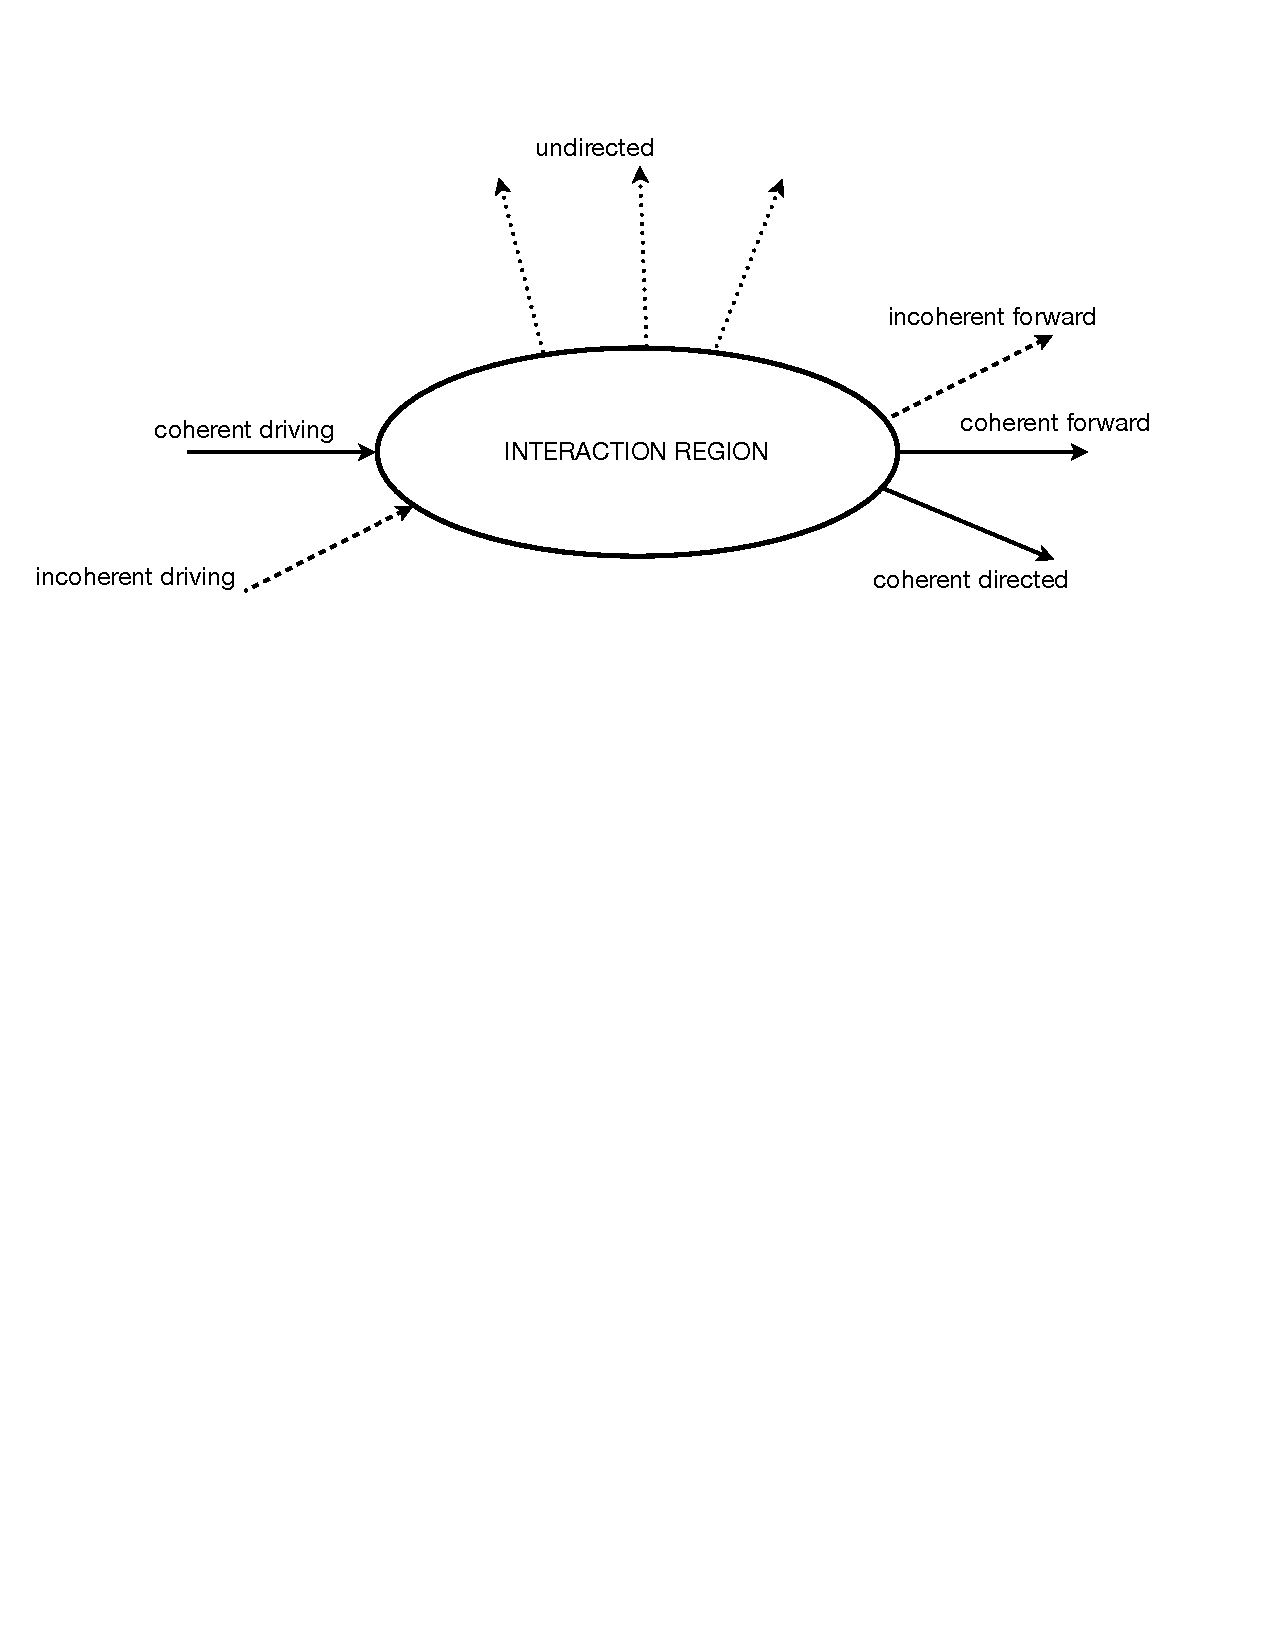
\includegraphics[width=0.8\textwidth]{Figures/2Scattering}
\caption[A schematic of a quantum optical scattering experiment]{\small{A schematic of a quantum optical scattering experiment. Different driving inputs enter the interaction region, such as a laser or other coherent electromagnetic field, while incoherent driving might represent incoming thermal photons. Coherent forward scattering could be indicative of stimulated emission, while undirected output might demonstrate spontaneous emission.}}
\label{fig2Scattering}
\end{center}
\end{figure}
%
Rather than monitoring the infinity of variables of which the system and reservoir composite consist, quantum trajectory theory allows us to measure only the inputs and outputs of a given quantum optical experiment \cite{howard2}. We follow the approach of Carmichael in \cite{howard2}, modeling an open quantum system and monitoring some of the environment. We cast the density operator of the system as a summation,
%
\be \rho(t) = \sum_i P_i \, \ket{\psi_i} \bra{\psi_i}, \label{eq2.48} \ee
%
where $P_i$ is the probability to find the system in state $\ket{\psi_i}$. However, this is not the unique form we require, which we can justify by considering a laser emitting a perfectly coherent state such that \eqref{eq2.48} becomes
%
\be \rho(t) = \int P_{\alpha} \, \ket{\psi_{\alpha}} \bra{\psi_{\alpha}} \, d\alpha = \sum_n P_n \, \ket{n} \bra{n}. \label{eq2.49} \ee
%
We are able to decompose the density operator into either coherent states or perfectly incoherent number states; this seems contradictory but is in fact true. Mathematically, this is merely a reflection of our ability to decompose a matrix into an infinite number of different bases; the coherent and number states represent two such possible choices.

However, the basis of most use in quantum trajectory theory is that of measurement records, denoted $\REC$, allowing us to restate \eqref{eq2.48} as
%
\be \rho(t) = \sum_{\REC} P_{\REC} \, \ket{\psi_{\REC}} \bra{\psi_{\REC}}. \label{eq2.50} \ee
%
The measurement record is a list of when the detector clicks for each event. In order to preserve probability, the trace over the density operator must sum to unity,
%
\be \sum_{\REC} P_{\REC} = 1. \label{eq2.51} \ee
%
In other words, the various weighting factors must sum to unity. It is important to understand that while the state vectors $\ket{\psi_{\REC}(t)}$ refer only to the system dynamics, the measurement record $\REC$ describes both the system and the reservoir. We require a density operator satisfying two conditions: (i) it must obey the master equation \eqref{eq2.46}, and (ii) yield probabilities $P_{\REC}$ that provide the correct weighting in relation to experimental results. The record must account for all observations, averages, and correlations. In order to evaluate the measurement record, we need to consider photon emissions.

First, we should examine the waiting time distribution. To construct it, we build a histogram using the time durations between subsequent clicks, i.e. from the $i$th click to the $(i + 1)$-click. Second, we need to consider the second-order correlation function $g^{(2)}(\tau)$, where the normalized form is defined in \cite{howard1} as
%
\[ g^{(2)}(\tau) = \frac{\langle \adag(t) \, \adag(t + \tau) \, a(t + \tau) \, a(t) \rangle}{ \left[ \langle \adag a \rangle(t) \right]^2}. \] 
%
The latter is best illustrated by constructing a histogram of the time durations between all pairs of clicks, whether they are sequential or not, i.e. from the $i$th click to the $j$th click.

To best describe the mathematical formalism of quantum trajectories, we begin by considering an Einstein stochastic process such as spontaneous emission \cite{howard2}. Stimulated emission is another such process, but does not allow for superposition, a constraint we do not wish to impose. We model spontaneous emission in the context of a two-state system with energy levels $\ket{1}$ and $\ket{2}$, defining $\gamma$ as the Einstein $A$ coefficient. Denoting the mean thermal photon number as $\bar{n}$, the respective probabilities to find the system in states $\ket{1}$ and $\ket{2}$ are $p_1$ and $p_2$, which obey the rate equations
%
\begin{subequations} \begin{align} 
\dot{p}_2 &= -\gamma_{\downarrow} p_2 + \gamma_{\uparrow} p_1, \label{eq2.52a} \\
\dot{p}_1 &= -\gamma_{\uparrow} p_1 + \gamma_{\downarrow} p_2, \label{eq2.52b} \end{align} \end{subequations}
%
where we have defined the transition rates
%
\be \gamma_{\downarrow} = \gamma \left( \bar{n} + 1 \right), \quad \gamma_{\uparrow} = \gamma \bar{n}. \label{eq2.53} \ee
%
One way to evaluate \eqref{eq2.52a} and \eqref{eq2.52b} is using a Monte Carlo simulation considering some time interval $t = b \, \delta t$, where $b$ is a counting variable and $\delta t$ is an infinitesimal time step. After each step, the simulation would proceed in a manner prescribed below after considering some random number $r_b$ in the range $r_b \in$ (0, 1):
%
\begin{subequations} \begin{align}
&\text{If } \ket{\psi(0)} = \ket{2}, \, p_{\downarrow} = \gamma_{\downarrow} \, \delta t. \text{ If } p_{\downarrow} > r_b, \text{ then } \ket{2} \to \ket{1}, \text{ else } \ket{2} \to \ket{2}; \label{eq2.54a} \\
&\text{If } \ket{\psi(0)} = \ket{1}, \, p_{\uparrow} = \gamma_{\uparrow} \, \delta t. \text{ If } p_{\uparrow} > r_b, \text{ then } \ket{1} \to \ket{2}, \text{ else } \ket{1} \to \ket{1}. \label{eq2.54b} \end{align} \end{subequations}
%
A sampling of the overall measurement record can then be written as
%
\[ \REC = \left\{ \begin{matrix} \cdots \\ \cdots \end{matrix}, \ \es, \ \begin{matrix} \gamma_{\uparrow} \\ T_{k-1} \end{matrix}, \ \es, \ \begin{matrix} \gamma_{\downarrow} \\ T_k \end{matrix}, \ \es, \ \begin{matrix} \gamma_{\uparrow} \\ T_{k+1} \end{matrix}, \ \es, \ \begin{matrix} \cdots \\ \cdots \end{matrix} \right. , \]
%
where $\es$ indicates an interval without photon detection, the $\gamma$'s mark the direction of the jump, and the $T$'s denote the time at which the jump occurred. This record consists of alternating raising and lowering jumps separated by intervals of non-detection. The density operator of \eqref{eq2.48} may now be written for our two-state system as
%
\be \rho(t) = p_1(t) \, \ket{1} \bra{1} + p_2(t) \, \ket{2} \bra{2}. \label{eq2.55} \ee
%
However, these are unconditional states and probabilities, making no reference to the measurement record; note that $p_1(t)$ and $p_2(t)$ obey the rate equations \eqref{eq2.52a} and \eqref{eq2.52b}. We want to connect \eqref{eq2.50} and \eqref{eq2.55} using the limiting case of $\bar{n} = 0$.

\subsection{Trajectories of a Known Initial State}
We first determine the conditional evolution of the system under a known initial state. There must then be three types of measurement records:
%
\be \begin{split} \recA &= \left\{ \begin{matrix} \ket{2} \\ 0 \end{matrix}, \ \es_t \right\}, \\ 
\recB &= \left\{ \begin{matrix} \ket{1} \\ 0 \end{matrix}, \ \es_t \right\}, \\ 
\recCTp &= \left\{ \begin{matrix} \ket{2} \\ 0 \end{matrix}, \ \es, \ \begin{matrix} \gamma \\ T' \end{matrix}, \ \es_t \right\}, \quad t' \leq T' < t' + dt. \label{eq2.56} \end{split} \ee
%
In record $\recA$, the system begins in state $\ket{2}$, no photons are detected out to time $t$, and the system remains in state $\ket{2}$; record $\recB$ is similar except the system begins and ends in state $\ket{1}$. For record $\recCTp$, the system begins in state $\ket{2}$, there is an interval of no photon detection, and then at time $T'$ there is a detector click and the system returns to state $\ket{1}$. It is now possible to write the unconditional state probabilities in terms of the three record types from \eqref{eq2.56}:
%
\begin{subequations} \begin{align} p_2(t) &= P(\recA) \, p_{2\vert\recA}(t) + P(\recB) \, p_{2\vert\recB}(t) + \int_0^t P(\recCTp) \, p_{2\vert\recCTp}(t) \, dt', \label{eq2.57a} \\
p_1(t) &= P(\recA) \, p_{1\vert\recA}(t) + P(\recB) \, p_{1\vert\recB}(t) + \int_0^t P(\recCTp) \, p_{1\vert\recCTp}(t) \, dt', \label{eq2.57b} \end{align} \end{subequations}
%
where the conditional probability $p_{i\vert\{ J \}}(t)$ indicates the probability for the system to be found in state $\ket{i}$ at time $t$ given the measurement record $\{ J \}$. Quantum trajectories prove flexible in this way as such formalism is easily extended to investigations with higher numbers of states and record types. The conditional probabilities in our case will be
%
\be \begin{split} &p_{2\vert\recA}(t) = 1, \quad p_{2\vert\recB}(t) = 0, \quad p_{2\vert\recCTp}(t) = 0, \\
&p_{1\vert\recA}(t) = 0, \quad p_{1\vert\recB}(t) = 1, \quad p_{1\vert\recCTp}(t) = 1, \label{eq2.58} \end{split} \ee
%
while the probabilities for the three record types are
%
\begin{subequations} \begin{align}
P(\recA) &= p_2(t) = p_2(0) \, e^{-\gamma t}, \label{eq2.59a} \\
P(\recB) &= p_1(0) = 1 - p_2(0), \label{eq2.59b} \\
P(\recCTp) &= \gamma \, p_2(0) \, e^{-\gamma t'}. \label{eq2.59c} \end{align} \end{subequations}
%
It is important to understand the origin of \eqref{eq2.59c} as it is a nontrivial result. First, we write according to \eqref{eq2.51} that
%
\be P(\recA) + P(\recB) + \int_0^t P(\recCTp) \, dt' = 1. \label{eq2.60} \ee
%
Differentiating the latter condition with respect to $t$ we find
%
\be \frac{d}{dt} \, P(\recA) + \frac{d}{dt} \, P(\recB) + P(\recCTp) = 0, \label{eq2.61} \ee
%
and using the relatively more intuitive results of \eqref{eq2.59a} and \eqref{eq2.59b} this simplifies as
%
\be P(\recCTp) = \left. P(\recCTp) \right\rvert_{t=t'} = \gamma \, e^{-\gamma t'} \, p_2(0), \label{eq2.62} \ee
%
where $P(\recCTp)/p_2(0)$ is found to be the waiting time distribution for a spontaneous emission event, conditioned on the system being prepared in state $\ket{2}$.

We are now ready to write the density operator in the form prescribed by \eqref{eq2.50}, substituting $\ket{\psi_{\recA}}$ for state $\ket{2}$, as well as $\ket{\psi_{\recB}}$ and $\lvert \psi_{\recCTp} \rangle$ for state $\ket{1}$:
%
\be \rho(t) = P(\recA) \, \ket{\psi_{\recA}} \bra{\psi_{\recA}} + P(\recB) \, \ket{\psi_{\recB}} \bra{\psi_{\recB}} + \int_0^t P(\recCTp) \, \ket{\psi_{\recCTp}} \bra{\psi_{\recCTp}} \, dt', \label{eq2.63} \ee
%
which reveals only two classes of quantum trajectories for a known initial state: (i) those where the detector never clicks, and (ii) those where the detector clicks and a photon emission is observed. Truthfully, we could have surmised such a conclusion early on, but it is crucial we discuss the formalism in this simpler case so that we can proceed to investigate systems of unknown initial states.

\subsection{Trajectories of an Unknown Initial State}
In this more complicated case, there are only two types of measurement records,
%
\be \begin{split} \recD &= \left\{ \tensor[_0]{\es}{_t} \right\}, \\
\recETp &= \left\{ \tensor[_0]{\es}{}, \ \begin{matrix} \gamma \\ T' \end{matrix}, \ \es_t \right\}, \label{eq2.64} \end{split} \ee
%
in contrast to the three possible record types of \eqref{eq2.56} with known initial states. The notation $\tensor[_0]{\es}{_t}$ denotes a time interval [0, $t$) without photon detection, while $\tensor[_0]{\es}{}$ indicates no other photon detections occurred from $t = 0$ until $t = T'$. The unconditional probabilities to be found in states $\ket{2}$ and $\ket{1}$ are highly similar to \eqref{eq2.57a} and \eqref{eq2.57b},
%
\begin{subequations} \begin{align} 
p_2(t) &= P(\recD) \, p_{2\vert\recD}(t) + \int_0^t P(\recETp) \, p_{2\vert\recETp}(t) \, dt', \label{eq2.65a} \\
p_1(t) &= P(\recD) \, p_{1\vert\recD}(t) + \int_0^t P(\recETp) \, p_{1\vert\recETp}(t) \, dt'. \label{eq2.65b} \end{align} \end{subequations}
%
The conditional probabilities for record $\recETp$ are easily written down, with $p_{2\vert\recETp}(t) = 0$ and $p_{1\vert\recETp}(t) = 1$ indicating the detection of a photon. The probabilities of the two records are also simply determined using the results of \eqref{eq2.59a}-\eqref{eq2.59c},
%
\begin{subequations} \begin{align}
P(\recD) &= P(\recA) + P(\recB) = p_2(0) \, e^{-\gamma t} + p_1(0), \label{eq2.66a} \\
P(\recETp) &= P(\recCTp) = \gamma \, e^{-\gamma t'} \, p_2(0). \label{eq2.66b} \end{align} \end{subequations}
%
The conditional probabilities of record $\recD$ are best determined using Bayes' theorem, which we state as
%
\be P(y) \, P(x\vert y) = P(x\wedge y), \label{eq2.67} \ee
%
where $P(x\vert y)$ is the probability of $x$ given $y$, and $P(x \wedge y)$ is the probability of $x$ and $y$. As a result, we can write
%
\be p_{2\wedge\recD}(t) = P(\recD) \, p_{2\vert\recD}(t), \label{eq2.68} \ee
%
where the system is found in state $\ket{2}$ and measurement record $\recD$. In fact, \eqref{eq2.68} is equal to the total probability to find the system in state $\ket{2}$, as
%
\[ p_2(t) = p_{2\vert\recD}(t) \, P(\recD) + p_{2\vert\recETp}(t) \, P(\recETp) = p_{2\vert\recD}(t) \, P(\recD), \]
%
due to the zero value of $p_{2\vert\recETp}(t)$. Combining \eqref{eq2.66a}, \eqref{eq2.66b}, and \eqref{eq2.68}, we can now determine
%
\be p_2(t) = p_{2\vert\recD}(t) \left[ p_2(0) \, e^{-\gamma t} + p_1(0) \right], \label{eq2.69} \ee
%
such that the normalized conditional probabilities of the two states are
%
\begin{subequations} \begin{align}
p_{2\vert\recD}(t) &= \frac{p_2(0) \, e^{-\gamma t}}{p_2(0) \, e^{-\gamma t} + p_1(0)}, \label{eq2.70a} \\
p_{1\vert\recD}(t) &= \frac{p_1(0)}{p_2(0) \, e^{-\gamma t} + p_1(0)}. \label{eq2.70b} \end{align} \end{subequations}
%

\subsection{Trajectories and the Master Equation}
We must now make the crucial step of incorporating quantum trajectories into the master equation, thereby combining Sections 2.1 and 2.2. First, note that we may rewrite \eqref{eq2.46} as
%
\[ \dot{\rho} = \sL\rho, \]
%
where $\sL$ is a superoperator and we use the Schr\"{o}dinger picture for this part of the discussion. One could feasibly break the superoperator up into two pieces, one representing the between-jump time evolution of the system, $\sL_B$, and another representing the effect of a jump, $\sL_{\gamma}$, such that
%
\be \dot{\rho} = \left( \sL_B + \sL_{\gamma} \right) \rho, \label{eq2.71} \ee
%
where we choose the specific superoperators
%
\be \begin{split} \sL_B \rho &= -\frac{i\omega_0}{2} \comm{\sigma_z}{\rho} - \frac{\gamma}{2} \left( \splus\sminus \rho + \rho \splus\sminus \right), \\
\sL_{\gamma} \rho &= \gamma \, \sminus \rho \splus. \label{eq2.72} \end{split} \ee
%
For $\sL_B$, the commutator term represents a standard quantum optical Hamiltonian, the $\gamma/2$ term comes from Bayes' theorem, and $\sL_{\gamma}$ causes jumps in the system. Note that the $\sigma$'s are Pauli pseudospin operators.

Returning to the interaction picture, we define a new density operator $\bar{\rho}$ such that
%
\be \bar{\rho} \equiv e^{-\sL_B t} \rho, \label{eq2.73} \ee
%
whose time derivative is
%
\[ \dot{\bar{\rho}} = e^{-\sL_B t} \dot{\rho} - \sL_B \, e^{-\sL_B t} \rho. \]
%
According to the superoperator form of the master equation, this becomes
%
\[ \dot{\bar{\rho}} = e^{-\sL_B t} \left( \sL_B + \sL_{\gamma} \right) \rho - \sL_B \, e^{-\sL_B t} \rho, \]
%
and using the fact that $\sL_B$ commutes with itself and its own exponential this expression simplifies as
%
\[ \dot{\bar{\rho}} = e^{-\sL_B t} \, \sL_{\gamma} \rho. \]
%
With a clever bit of multiplication, this becomes
%
\[ \dot{\bar{\rho}} = e^{-\sL_B t} \, \sL_{\gamma} \, e^{\sL_B t} \, e^{-\sL_B t} \rho, \]
%
or finally
%
\be \dot{\bar{\rho}} = e^{-\sL_B t} \, \sL_{\gamma} \, e^{\sL_B t} \bar{\rho}, \label{eq2.74} \ee
%
which is the superoperator form of the master equation in the interaction picture. We now wish to solve for $\bar{\rho}$ and perform a change of basis back to the Schr\"{o}dinger picture and $\rho$. In order to accomplish this, we use time-dependent perturbation theory. Integrating both sides of \eqref{eq2.74} with respect to time,
%
\be \int_0^t \frac{d}{dt'} \bar{\rho}(t') \, dt' = \int_0^t e^{-\sL_B t'} \, \sL_{\gamma} \, e^{\sL_B t'} \bar{\rho}(t') \, dt', \label{eq2.75} \ee
%
or
%
\be \bar{\rho}(t) = \bar{\rho}(0) + \int_0^t e^{-\sL_B t'} \, \sL_{\gamma} \, e^{\sL_B t'} \bar{\rho}(t') \, dt'. \label{eq2.76} \ee
%
We transform back to the Schr\"{o}dinger picture by substituting \eqref{eq2.73} into \eqref{eq2.76} and finding
%
\be e^{-\sL_B t} \rho(t) = \rho(0) + \int_0^t e^{-\sL_B t'} \, \sL_{\gamma} \rho(t') \, dt', \label{eq2.77} \ee
%
or
%
\be \rho(t) = e^{\sL_B t} \rho(0) + \int_0^t e^{\sL_B (t - t')} \, \sL_{\gamma} \rho(t') \, dt'. \label{eq2.78} \ee
%
Now, we substitute $\rho(t)$ from the left-hand side into $\rho(t')$ on the right-hand side to obtain
%
\be \rho(t) = e^{\sL_B t} \rho(0) + \int_0^t e^{\sL_B (t - t')} \, \sL_{\gamma} \left[ e^{\sL_B t'} \rho(0) + \int_0^t e^{\sL_B (t' - t'')} \, \sL_{\gamma} \rho(t'') \, dt'' \right] dt'. \label{eq2.79} \ee
%
In a standard perturbation theory approach, it would be necessary to make such a substitution an infinite number of times to exactly solve for $\rho(t)$. However, a property of record $\recETp$, referring back to \eqref{eq2.64}, renders this unnecessary. The outer integral, i.e. the $dt'$ one, tracks all possible times up to $T'$ we expect to detect a photon, after which the system is in state $\ket{1}$ with certainty. This means integrating $\sL_{\gamma}$ at any time after $T'$ results in a zero value, and as such the inner, or $dt''$, integral vanishes, leaving only
%
\be \rho(t) = e^{\sL_B t} \rho(0) + \int_0^t e^{\sL_B (t - t')} \, \sL_{\gamma} \, e^{\sL_B t'} \rho(0) \, dt', \label{eq2.80} \ee
%
which can be solved analytically.

We pause briefly at this point to calculate four quantities of note that will soon prove useful. Recalling that the density operator initially has the form
%
\[ \rho(0) = p_2(0) \, \ket{2} \bra{2} + p_1(0) \, \ket{1} \bra{1}, \] 
%
it is possible to show
%
\be \sL_B \, \ket{2} \bra{2} = -\gamma \, \ket{2} \bra{2}, \quad \sL_B \, \ket{1} \bra{1} = 0, \quad \sL_{\gamma} \, \ket{2} \bra{2} = \gamma \, \ket{1} \bra{1}, \quad \sL_{\gamma} \, \ket{1} \bra{1} = 0. \label{eq2.81} \ee
%
Using $\rho(0)$ and \eqref{eq2.81}, we are now capable of representing the two types of records in operator notation. For record $\recD$ we can write
%
\be e^{\sL_B t} \rho(0) = e^{-\gamma t} \, p_2(0) \, \ket{2} \bra{2} + p_1(0) \, \ket{1} \bra{1}; \label{eq2.82} \ee
%
similarly, record $\recETp$ follows from
%
\begin{align} e^{\sL_B (t - t')} \, \sL_{\gamma} \, e^{\sL_B t'} \rho(0) &= e^{\sL_B (t - t')} \, \sL_{\gamma} \left[ e^{-\gamma t'} \, p_2(0) \, \ket{2} \bra{2} + p_1(0) \, \ket{1} \bra{1} \right] \nonumber \\
&= e^{\sL_B (t - t')} \, \gamma \, e^{-\gamma t'} \, p_2(0) \, \ket{1} \bra{1} \nonumber \\
&= \gamma \, e^{-\gamma t'} \, p_2(0) \, \ket{1} \bra{1}. \label{eq2.83} \end{align}
%
The probabilities for the two measurement records can be calculated both by taking traces,
%
\be \begin{split} P(\recD) &= \tr \left[ e^{\sL_B t} \rho(0) \right], \\
P(\recETp) &= \tr \left[ e^{\sL_B (t - t')} \, \sL_{\gamma} \, e^{\sL_B t'} \rho(0) \right], \label{eq2.84} \end{split} \ee
%
and using Dirac notation,
%
\be \begin{split} P(\recD) &= \bra{2} \, e^{\sL_B t} \rho(0) \, \ket{2} + \bra{1} \, e^{\sL_B t} \rho(0) \ket{1} = e^{-\gamma t} \, p_2(0) + p_1(0) \\
P(\recETp) &= \bra{2} \, \bar{\sL}_{\gamma} \rho(0) \, \ket{2} + \bra{1} \, \bar{\sL}_{\gamma} \rho(0) \, \ket{1} = \gamma \, e^{-\gamma t'} \, p_2(0), \label{eq2.85} \end{split} \ee
%
where we have defined $\bar{\sL}_{\gamma} \equiv e^{\sL_B (t - t')} \, \sL_{\gamma} \, e^{\sL_B t'}$. The normalized, conditional density operators can be calculated by
%
\be \rho_{\recD}(t) = \frac{e^{\sL_B t} \rho(0)}{P(\recD)}, \quad \rho_{\recETp}(t) = \frac{\bar{\sL}_{\gamma} \rho(0)}{P(\recETp)}, \label{eq2.86} \ee
%
using the results of \eqref{eq2.85}.

\subsection{Trajectories and Pure States}
We now want to understand quantum trajectories in the context of coherence, and do so by considering an arbitrary initial pure state $\ket{\psi}$. Applying our between-jump superoperator from \eqref{eq2.72} yields
%
\begin{align} \sL_B \, \ket{\psi} \bra{\psi} &= -\frac{i\omega_0}{2} \comm{\sigma_z}{\ket{\psi} \bra{\psi}} - \frac{\gamma}{2} \left( \splus\sminus \ket{\psi} \bra{\psi} + \ket{\psi} \bra{\psi} \splus\sminus \right) \nonumber \\
&= -\frac{i\omega_0}{2} \sigma_z \ket{\psi} \bra{\psi} + \frac{i\omega_0}{2} \ket{\psi} \bra{\psi} \sigma_z - \frac{\gamma}{2} \splus\sminus \ket{\psi} \bra{\psi} - \frac{\gamma}{2} \ket{\psi} \bra{\psi} \splus\sminus \nonumber \\
&= -\frac{i}{\hbar} \left( \frac{\hbar\omega_0}{2} \sigma_z - i\hbar \frac{\gamma}{2} \splus\sminus \right) \ket{\psi} \bra{\psi} + \frac{i}{\hbar} \, \ket{\psi} \bra{\psi} \left( \frac{\hbar\omega_0}{2} \sigma_z + i\hbar \frac{\gamma}{2} \splus\sminus \right) \nonumber \\
&= -\frac{i}{\hbar} H_B \ket{\psi} \bra{\psi} + \frac{i}{\hbar} \ket{\psi} \bra{\psi} H^{\dag}_B, \label{eq2.87} \end{align}
%
where we have defined the non-Hermitian Hamiltonian
%
\be H_B \equiv \frac{\hbar\omega_0}{2} \sigma_z - i\hbar \frac{\gamma}{2} \splus\sminus. \label{eq2.88} \ee
%
We can also apply the propagator of \eqref{eq2.82} to our pure state to obtain
%
\be e^{\sL_B t} \ket{\psi} \bra{\psi} = \ket{\psi_t} \bra{\psi_t}, \label{eq2.89} \ee
%
where we have defined a new state
%
\be \ket{\psi_t} \equiv e^{-iH_B t/\hbar} \, \ket{\psi}. \label{eq2.90} \ee
%
Note that \eqref{eq2.87} is effectively the Schr\"{o}dinger equation with a non-Hermitian Hamiltonian. More importantly, \eqref{eq2.90} reflects a pure state, indicating that if record $\recD$ begins with a pure state, it must also end with one.

Next we consider the jump superoperator acting on a pure state,
%
\be \sL_{\gamma} \ket{\psi} \bra{\psi} = \gamma \, \sminus \ket{\psi} \bra{\psi} \splus = \ket{\psi_{\gamma}} \bra{\psi_{\gamma}}, \label{eq2.91} \ee
%
where we have defined a second new state
%
\be \ket{\psi_{\gamma}} \equiv J_{\gamma} \ket{\psi} = \sqrt{\gamma} \, \sminus \ket{\psi}. \label{eq2.92} \ee
%
Just as with \eqref{eq2.90}, the jump operator of \eqref{eq2.92} changes one pure state into another. In general, whether record $\recD$ or $\recETp$ occurs, starting with a pure state will always conclude with another pure state.

If we substitute \eqref{eq2.89} into \eqref{eq2.84} for record $\recD$, we can use the cyclic property of the trace and the fact that the trace of a number is that same number to determine the probability of $\recD$ as
%
\begin{align} P(\recD) &= \tr \left[ e^{\sL_B t} \rho(0) \right] \nonumber \\
&= \tr \left\{ \ket{\psi_t} \bra{\psi_t} \right\} \nonumber \\
&= \tr \left\{ \braket{\psi_t}{\psi_t} \right\} \nonumber \\
&= \braket{\psi_t}{\psi_t} \nonumber \\
&= \braket{\bar{\psi}_{\recD}}{\bar{\psi}_{\recD}}, \label{eq2.93} \end{align}
%
where we have defined the unnormalized, conditional pure state
%
\be \ket{\bar{\psi}_{\recD}} \equiv e^{-iH_B t/\hbar} \, \ket{\psi} = e^{i\omega_0 t/2} \, c_1(0) \, \ket{1} + e^{-i\omega_0 t/2} \, e^{-\gamma t/2} \, c_2(0) \, \ket{2}. \label{eq2.94} \ee
%
For measurement record $\recETp$ we obtain a second unnormalized, conditional pure state
%
\begin{align} \ket{\bar{\psi}_{\recETp}} &= e^{iH_B (t - t')/\hbar} \, J_{\gamma} \, e^{-iH_B t'/\hbar} \, \ket{\psi(0)} \nonumber \\
&= e^{iH_B (t - t')/\hbar} \, J_{\gamma} \left[ e^{i\omega_0 t'/2} \, c_1(0) \, \ket{1} + e^{-i\omega_0 t'/2} \, e^{-\gamma t'/2} \, c_2(0) \, \ket{2} \right] \nonumber \\
&= e^{iH_B (t - t')/\hbar} \, \sqrt{\gamma} \, e^{-i\omega_0 t'/2} \, e^{-\gamma t'/2} \, c_2(0) \, \ket{1} \nonumber \\
&= \sqrt{\gamma} \, e^{-i\omega_0 t'/2} \, e^{-\gamma t'/2} \, e^{i\omega_0 (t - t')/2} \, c_2(0) \, \ket{1}. \label{eq2.95} \end{align}
%
All the formalism of Section 2.2.4 stems from the generalized Lindblad form of the master equation analogous to that of \eqref{eq2.47},
%
\be \dot{\rho} = -\frac{i}{\hbar} \comm{H_0}{\rho} + \sum_i \frac{\gamma_i}{2} \left( 2 \hat{O}_i \rho \hat{O}^{\dag}_i - \hat{O}^{\dag}_i \hat{O}_i \rho - \rho \hat{O}^{\dag}_i \hat{O}_i \right), \label{eq2.96} \ee
%
which can be broken into two respective pieces describing the time evolution between jumps and the jumps themselves,
%
\begin{subequations} \begin{align}
\sL_B \rho &= -\frac{i}{\hbar} \comm{H_0}{\rho} - \sum_i \frac{\gamma_i}{2} \left( \hat{O}^{\dag}_i \hat{O}_i \rho + \rho \hat{O}^{\dag}_i \hat{O}_i \right), \label{eq2.97a} \\
\sL_i \rho &= \gamma_i \, \hat{O}_i \rho \hat{O}^{\dag}_i. \label{eq2.97b} \end{align} \end{subequations}
%
The generalized density operator for a given measurement record will take the form
%
\be \bar{\rho}_{\REC}(t) = \cdots \sL_{i_2} \, e^{\sL_B (t_2 - t_1)} \, \sL_{i_1} \, e^{\sL_B t_1} \, \rho(0), \label{eq2.98} \ee
%
with unnormalized, conditional state vector
%
\be \ket{\bar{\psi}_{\REC}(t)} = \cdots J_{i_2} \, e^{-iH_B (t_2 - t_1)/\hbar} \, J_{i_1} \, e^{-iH_B t_1/\hbar} \, \ket{\psi(0)}, \label{eq2.99} \ee
%
and probability to obtain the measurement record of
%
\be P(\REC) = \braket{\bar{\psi}_{\REC}(t)}{\bar{\psi}_{\REC}(t)}. \label{eq2.100} \ee
%
In order to numerically analyze the trajectories for an initial pure state, we begin with some state $\ket{\psi(t)}$, and after a minuscule time increment $\delta t$, either perform a jump or apply the propagator. The probability for a jump to occur is
%
\be P_J = \braket{\bar{\psi}_J}{\bar{\psi}_J} = \bra{\psi(t)} \, J^{\dag} J \, \ket{\psi(t)} \, \delta t, \label{eq2.101} \ee
%
where
%
\be J \, \ket{\psi(t)} = \ket{\overline{\psi_J(t + \delta t)}}, \label{eq2.102} \ee
%
or more explicitly
%
\be e^{-iH_B (\delta t - t')/\hbar} \, J_{i_1} \, e^{-iH_B t'/\hbar} \, \ket{\psi(0)} = \left[ 1 - O(\delta t) \right] J_{i_1} \left[ 1 - O(\delta t) \right] \ket{\psi(0)} = J_{i_1} \, \ket{\psi(0)}. \label{eq2.103} \ee
%
The terms of order $O(\delta t)$ can be ignored due to their weak dependence on $t'$, i.e. $\delta t$ represents an incredibly small time interval. After a single jump in time $\delta t$, the probability for the measurement record is
%
\begin{align} P(\REC) &= \int_0^{\delta t} \braket{\psi_{t'}}{\psi_{t'}} \, dt' \nonumber \\
&= \int_0^{\delta t} \bra{\psi(0)} \, J^{\dag} J \, \ket{\psi(0)} \, dt' \nonumber \\
&= \bra{\psi} \, J^{\dag} J \, \ket{\psi} \, \delta t \nonumber \\
&= \gamma \, \evalue{\splus\sminus} \, \delta t, \label{eq2.104} \end{align}
%
where $\gamma$ must have the units of a rate. The probability of a record with no jump is easily calculated to be
%
\[ P(\REC) = 1 - P_J, \]
%
and results in only a minor correction to the initial state vector of the form
%
\[ \ket{\psi} \to \left( 1 - \frac{i}{\hbar} H_B \, \delta t \right) \ket{\psi}. \]
%
Now that we have developed the necessary formalism of quantum trajectories as per Carmichael in \cite{howard2}, we are ready to interrogate the heart of this discussion, the theory behind cavity optomechanics.

\section{Cavity Optomechanics}
The field of cavity optomechanics has arisen in recent years as a specific niche of quantum optics, which seeks to study the coupling of mechanical degrees of freedom to the modes of optical cavities, primarily via (i) radiation pressure, (ii) optical gradients, or (iii) photothermal force \cite{girvin2011}. This thesis focuses exclusively on the first mechanism. Such studies are motivated by the construction of sensitive mass and force sensors, and in quantum computation in order to supply long-range interaction between qubits \cite{girvin2011}. Experimental and theoretical investigations have also been proposed to probe the nature of quantum mechanics at larger mass scales \cite{corbitt2007, girvin2011}. In the standard cOM apparatus, the position of a mechanical oscillator modulates the frequency of an optical cavity mode \cite{girvin2011}. Such coupling is typically small relative to the mechanical frequency and cavity linewidth \cite{girvin2011}.

We follow the approach of \cite{girvin2011}, using the standard model of optomechanics: the position of the mechanical oscillator is, in operator notation,
%
\be \hat{x} = x_{\ZPF} \left( b + \bdag \right), \label{eq2.105} \ee
%
where $b$ ($\bdag$) is the bosonic annihilation (creation) operator for mechanical oscillator phonon excitations and $x_{\ZPF} = \sqrt{\hbar/2M\omega_M}$ is the zero-point uncertainty in the position, which includes the oscillator mass $M$. For a single cavity mode $a$ linearly coupled to the oscillator, the Hamiltonian is
%
\be H_0 = \hbar\omega \, \adag a + \hbar\omega_M \, \bdag b + g_M \, \adag a \left( b + \bdag \right), \label{eq2.106} \ee
%
where $\omega$ is the frequency of the driving field and $\omega_M$ is the frequency of the mechanical oscillator. The optomechanical coupling $g_M = \omega' x_{\ZPF}$ is defined using the partial derivative $\omega' = \partial\omega/\partial x$, i.e. the frequency modulation due to the change in position of the oscillator.

It is of note that the Hamiltonian \eqref{eq2.106} conserves photon number, i.e. it commutes with the photon number operator $\adag a$. The Hamiltonian is perhaps best conceived as a displacement in position of a harmonic oscillator of frequency $\omega_M$; the magnitude of this displacement is given by $-nx_0$, where $n$ is the photon number and $x_0 = 2x_{\ZPF}g/\omega_M$ is a single-photon displacement. Such an interpretation arises from diagonalizing the Hamiltonian in the subspace of $n$ photons.

As the authors point out in \cite{girvin2011}, the optical probe spectrum of this cOM system will display  sideband peaks at integer multiples of $\omega_M$ whose widths are multiples of the mechanical linewidth, which we denote $\kappa_M$. In the temperature limit $T \to 0$, the peaks will only appear at frequencies redshifted from the driving frequency $\omega$. This occurs because photons can only create phonons, and as a result leave the cavity with an output frequency $\omega_{\text{out}} < \omega$. For temperature $T > 0$, or for stronger driving, additional sideband peaks will arise blueshifted from $\omega$, due to nonzero probability for a photon to absorb the energy of one or more phonons, leaving the cavity with frequency $\omega_{\text{out}} > \omega$.

In our model of cOM, we consider a weakly-driven single-mode cavity, where the field mode is coupled to a single two-level atom via the Jaynes-Cummings coupling rate $g$ and to the mechanical oscillator with rate $g_M$. The full optomechanical Hamiltonian, including driving, both types of coupling, and dissipation through (i) spontaneous emission of the atom, (ii) loss of a photon from the cavity mode, or (iii) loss of a phonon from the oscillator, can be written as
%
\be \begin{split} H &= \hbar\Delta \left( \adag a + \splus\sminus \right) + \hbar\omega_M \, \bdag b + \hbar Y \left( a + \adag \right) + \hbar g \left( a\splus + \adag\sminus \right) \\ &\qquad + \hbar g_M \, \adag a \left( b + \bdag \right) - i\hbar\kappa \, \adag a - i\hbar\frac{\gamma}{2} \, \splus\sminus - i\hbar\frac{\kappa_M}{2} \, \bdag b. \label{eq2.107} \end{split} \ee
%
The majority of the parameters in \eqref{eq2.107} have been mentioned earlier in Section 1, but we have introduced the detuning $\Delta = \omega - \omega_0$, i.e. the frequency offset between the driving field and the resonant cavity mode and atomic transition. Our choice of interaction picture is defined by entering a frame rotating at frequency $\omega$, such that the atomic term $(\hbar\omega_0/2) \, \sigma_z$ and cavity term $\hbar\omega \, \adag a$ vanish, assuming the cavity mode and atomic transition are resonant, i.e. $\omega = \omega_0$. Note that by including damping terms the Hamiltonian has become non-Hermitian just as in \eqref{eq2.88}. 

Now that we have developed the necessary theoretical tools and formalism, we are ready to tackle an investigation of the system represented by \eqref{eq2.107}. It will be possible, using the QuTiP software package \cite{qutipref}, to vary one or more parameters and consider the effects on various output such as the probe spectra and correlation functions. In the chapter that follows, we will consider two types of classical mechanical oscillators as a limiting case before commencing a full quantum treatment of the composite atom-field-oscillator system.
\chapter{Classical Oscillator}
We begin our investigation of a cOM apparatus by first modeling a classical mechanical oscillator. Our approach is to transform operators into conventional classical functions, and we do so using two different methods. First, the standard cQED apparatus is mechanically coupled to a harmonic oscillator following a sine function. Second, the oscillator is placed in a thermal state and undergoes Brownian motion using a pseudorandom number generator. Plots of mean photon number of the cavity mode and mean atomic excitation number over time provide baseline dynamics that can be compared when the oscillator is written using operator formalism.

\section{Harmonic Oscillator}
For a sinusoidal oscillator, we consider the necessary modifications to the Hamiltonian of \eqref{eq2.107}. Appealing to simplicity, we consider a driving field resonant with the cavity mode and atomic transition, such that the $\Delta$ term vanishes. Because the $\hbar\omega_M \, \bdag b$ term reflects an internal energy of the mechanical oscillator, we may, in the classical picture, conceive of it as an energy offset to the Hamiltonian; this could be subtracted away in an experimental apparatus and as such we disregard the $\bdag b$ term as well. Lastly, because we take the oscillator to be at zero temperature, the $\kappa_M$ term is omitted. This leaves us with the driving term, two coupling terms, and two modes of dissipation,
%
\be \begin{split} H'_{\text{harmonic}} &= \hbar Y \left( a + \adag \right) + \hbar g \left( a\splus + \adag\sminus \right) + \hbar g_M \, \adag a \left( b + \bdag \right) \\
&\qquad - i\hbar\kappa \, \adag a - i\hbar\frac{\gamma}{2} \, \splus\sminus, \label{eq3.1} \end{split} \ee
%
where the prime denotes that we have yet to convert the position operator $\hat{x}$ of \eqref{eq2.105} to a classical function. For the sinusoidal case, the end mirror of the cavity oscillates with frequency $\omega_M$ such that \eqref{eq3.1} is now
%
\be \begin{split} H_{\text{harmonic}} &= \hbar Y \left( a + \adag \right) + \hbar g \left( a\splus + \adag\sminus \right) + \hbar g_M \, \adag a \, \sin(\omega_M t) \\
&\qquad - i\hbar\kappa \, \adag a - i\hbar\frac{\gamma}{2} \, \splus\sminus. \label{eq3.2} \end{split} \ee
%
Using QuTiP and the \texttt{odesolve} function, the Schr\"{o}dinger equation is numerically evaluated using Hamiltonian \eqref{eq3.2} to determine the expectation values $\langle \adag a \rangle$ and $\langle \splus\sminus \rangle$, whose traces are shown below.
%
\begin{figure}[htb]
\begin{center}
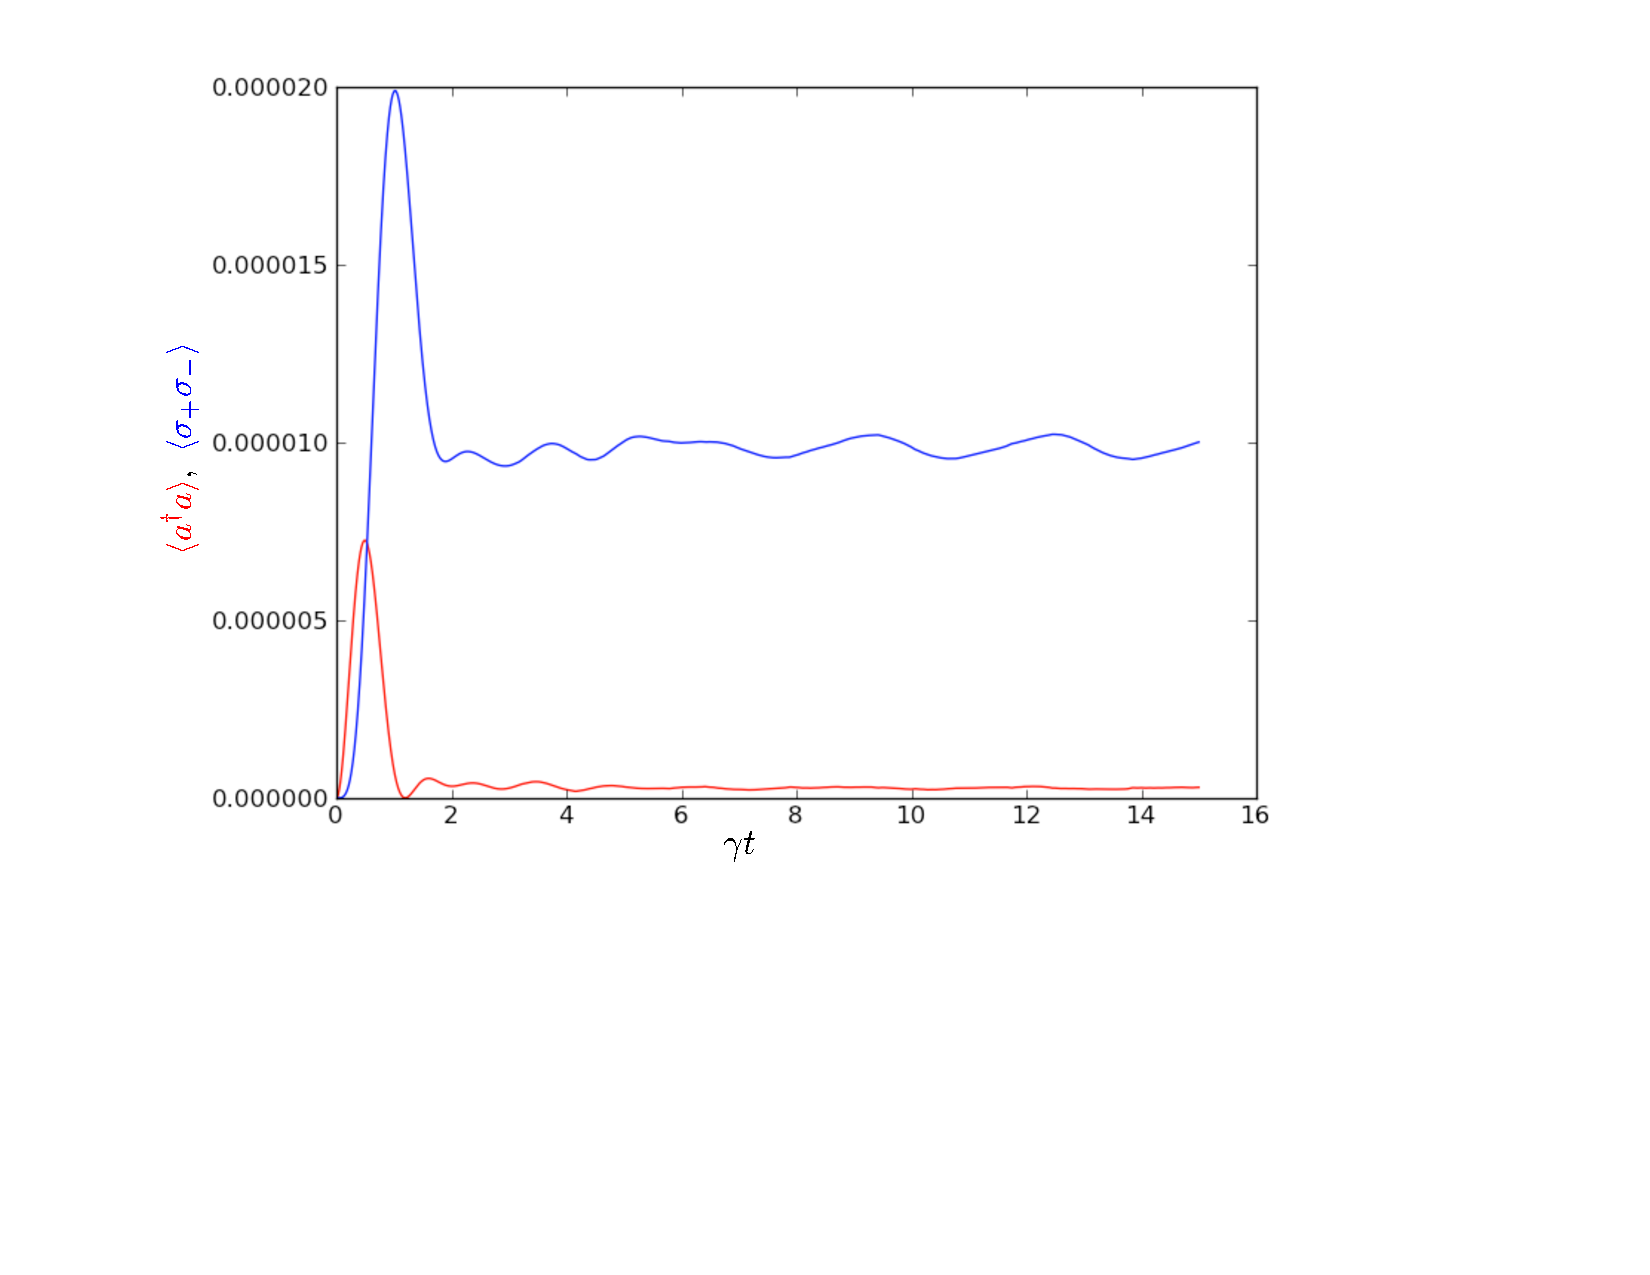
\includegraphics[width=0.85\textwidth]{Figures/3HarmonicPlots}
\caption[A plot of the expectation values $\langle \adag a \rangle$ and $\langle \splus\sminus \rangle$ for the harmonic oscillator]{\small{A plot of the expectation values $\langle \adag a \rangle$ and $\langle \splus\sminus \rangle$. The two quantities are calculated over fifteen spontaneous emission lifetimes; red denotes $\langle \adag a \rangle$ and blue denotes $\langle \splus\sminus \rangle$. The relevant parameters are $\gamma = \kappa = \omega_M = 1$, $Y/\gamma = 0.01$, $g/\gamma = 3$, and $g_M/\gamma = 2$.}}
\label{fig3Harmonic}
\end{center}
\end{figure}
%
In order to emphasize our consideration of weak driving, we will, in all cases, allow at most two excitations in the atom-cavity subsystem. Before we comment upon Fig.~\ref{fig3Harmonic}, we proceed to consider the next type of classical mechanical oscillator and its analogous plot.

\section{Thermal Oscillator}
In this second approach to the classical picture, we consider the situation where the oscillating end mirror is placed in a thermal state, i.e. the mirror undergoes Brownian motion. We will incorporate the same approximations as in Section~3.1, such that the preliminary Hamiltonian will be identical to \eqref{eq3.1}, or $H'_{\text{thermal}} = H'_{\text{harmonic}}$. To transform to a classical term as in \eqref{eq3.2}, we write
%
\be \begin{split} H_{\text{thermal}} &= \hbar Y \left( a + \adag \right) + \hbar g \left( a\splus + \adag\sminus \right) + \hbar g_M \, \adag a \, \xi \\
&\qquad - i\hbar\kappa \, \adag a - i\hbar\frac{\gamma}{2} \, \splus\sminus, \label{eq3.3} \end{split} \ee
%
where $\xi$ is a pseudorandom number generated by QuTiP in the range $\xi \in$ (0, 1) chosen once for each trajectory. Again as in Section~3.1, we calculated expectation values for the cavity mode and two-level atom over time. These traces are shown below.
%
\begin{figure}[htb]
\begin{center}
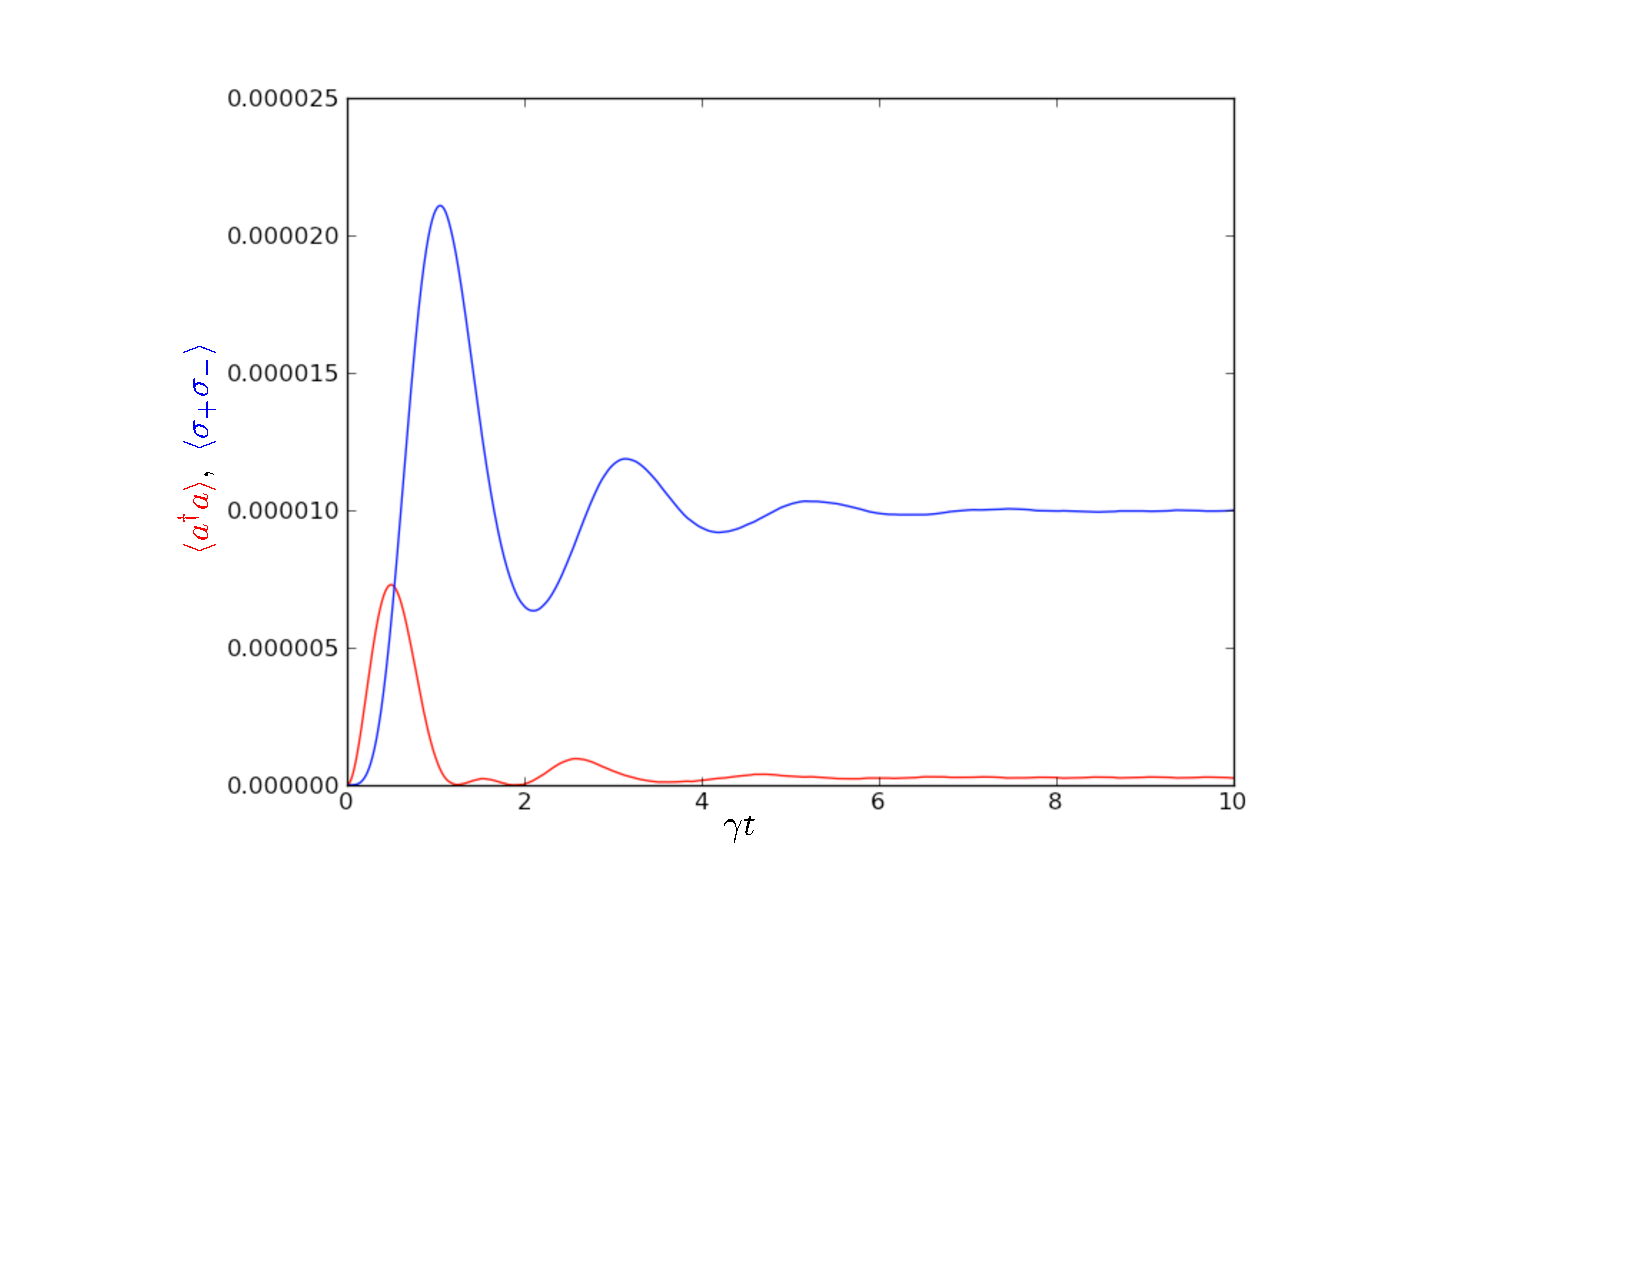
\includegraphics[width=0.85\textwidth]{Figures/4ThermalPlots}
\caption[A plot of the expectation values $\langle \adag a \rangle$ and $\langle \splus\sminus \rangle$ for the thermal oscillator]{\small{A plot of the expectation values $\langle \adag a \rangle$ and $\langle \splus\sminus \rangle$. The two quantities are calculated over ten spontaneous emission lifetimes; red denotes $\langle \adag a \rangle$ and blue denotes $\langle \splus\sminus \rangle$. The relevant parameters are identical to Fig.~\ref{fig3Harmonic} with the exception of $\omega_M$, which was not referenced in this calculation.}}
\label{fig4Thermal}
\end{center}
\end{figure}

We first consider the steady-state results of both figures. For the harmonic oscillator, the respective lengths of time for $\langle \adag a \rangle$ and $\langle \splus\sminus \rangle$ to settle are approximately $7\tau_0$ and $9\tau_0$, while in the thermal oscillator we see $6\tau_0$ and $8\tau_0$; we have introduced the spontaneous emission lifetime $\tau_0 = 1/\gamma$. Another important feature is that both plots lie in the same order of magnitude, we see $\langle \adag a \rangle$ and $\langle \splus\sminus \rangle \sim 10^{-5}$. It follows that Figs.~\ref{fig3Harmonic} and \ref{fig4Thermal} are similar in range and appearance, as their respective Hamiltonians \eqref{eq3.2} and \eqref{eq3.3} differ only by a constant factor in the $g_M$ coupling term. While \eqref{eq3.2} sees the coupling oscillate between $\pm 1$, the thermal oscillator \eqref{eq3.3} produces a constant coupling whose magnitude is dictated by $\xi$.

We have discovered baseline behavior for the mechanical oscillator in both the harmonic and thermal cases, where an initial excitation due to driving of the cavity mode pushes the mean cavity photon number and atomic excitation number settles to a steady-state value after fewer than ten spontaneous emission lifetimes of the atom. It would also prove useful to discuss experimental values for the various parameters of the system in order to provide some numerical perspective. The spontaneous emission rate is typically in the microwave region, on the order of 1-10 GHz, which also sets the scale for the cavity decay rate. Most versions of an experimental optomechanical apparatus realize mechanical frequencies $\omega_M$ on the order of 1-10 MHz \cite{arcizet2006, kippenberg2005, kimble2009}, but we follow the lead of \cite{thompson2007} in using mechanical frequencies on the order of $\gamma$ and $\kappa$. With these numbers in mind, we are now ready to proceed to a full quantum treatment of the cOM system.
\chapter{Quantum Mechanical Oscillator}
In this chapter, we perform a fully quantum mechanical analysis of the mechanical oscillator, investigating its characteristics with two primary methods. First, we calculate, using the \texttt{mcsolve} function of QuTiP, probe spectra of the cOM system using a range of optical and mechanical coupling values. These results can be compared to the vacuum Rabi doublet, a well-established theoretical \cite{mondragon1983, agarwal1984} and experimental \cite{thompson1992} result of the standard cQED model. Second, we consider the photon statistics of the atom-cavity-oscillator system, specifically the second-order correlation functions $g^{(2)}(0)$ and $g^{(2)}(\tau)$, denoting the respective statistical state of the system at equilibrium, i.e. in the steady state, and due to time evolution. These calculations may also be compared to theoretical results \cite{brecha1999} of the standard cQED realization. We also note that \texttt{mcsolve} is representative of our use of quantum trajectories in the aforementioned calculations, as the function performs Monte Carlo simulations of the desired Hamiltonian and initial state \cite{qutipref}.

\section{Probe Spectra}
To calculate probe spectra, we start by considering the full optomechanical Hamiltonian \eqref{eq2.107}. For reasons previously outlined in Section~3.1, we omit the $\kappa_M$ dissipation piece and opt to utilize all other terms in $H$. The three values calculated in the various spectra are $\langle \adag a \rangle$, $\langle \splus\sminus \rangle$, and $\langle \bdag b \rangle$, respectively the mean cavity photon number, the mean atomic excitation number, and the mean oscillator phonon number. In Fig.~\ref{fig5gM} we plot these expectation values for a set $g$ over a range of $g_M$. We find that for weak mechanical coupling, i.e. $g_M < g$, the spectra retain nearly the exact shape of the vacuum Rabi doublet, with peaks of linewidth $(\kappa + \gamma/2)/2$ centered nearly about $\pm g$ \cite{howard2}. In Fig.~\ref{fig5b} we see asymmetry beginning to appear, likely due to the previously mentioned inability of the cavity photons to take energy from the oscillator and as such becoming redshifted. As the oscillator becomes more strongly coupled, i.e. $g_M \geq g$, we see the sideband peaks at integer multiples of $\omega_M$ begin to emerge and become more distinct, also mentioned in Section~2.3.
\newpage
\begin{figure}[htb]
\centering
\subfloat[\small{$g_M/\gamma = 0.1$}]{\label{fig5a}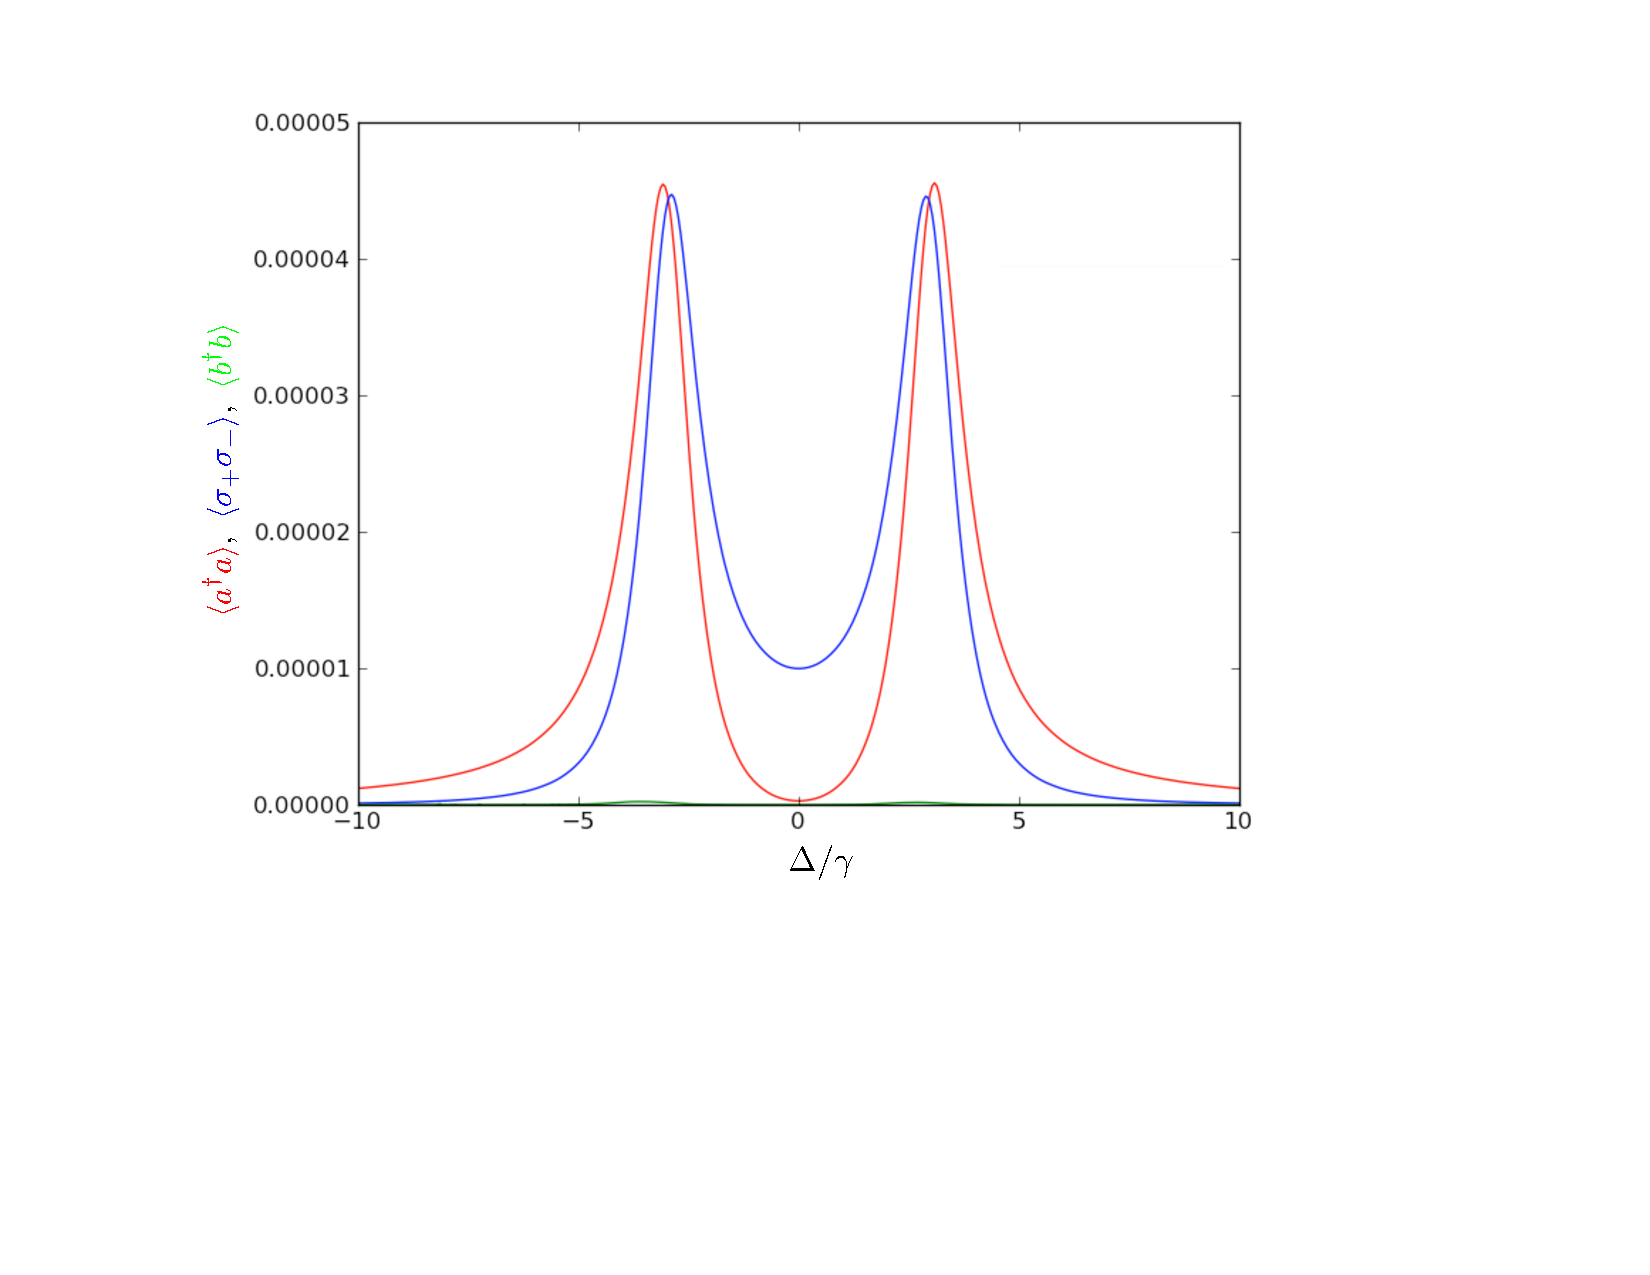
\includegraphics[width=0.474\textwidth]{Figures/5a_gM1_10}}
\qquad
\subfloat[\small{$g_M/\gamma = 1$}]{\label{fig5b}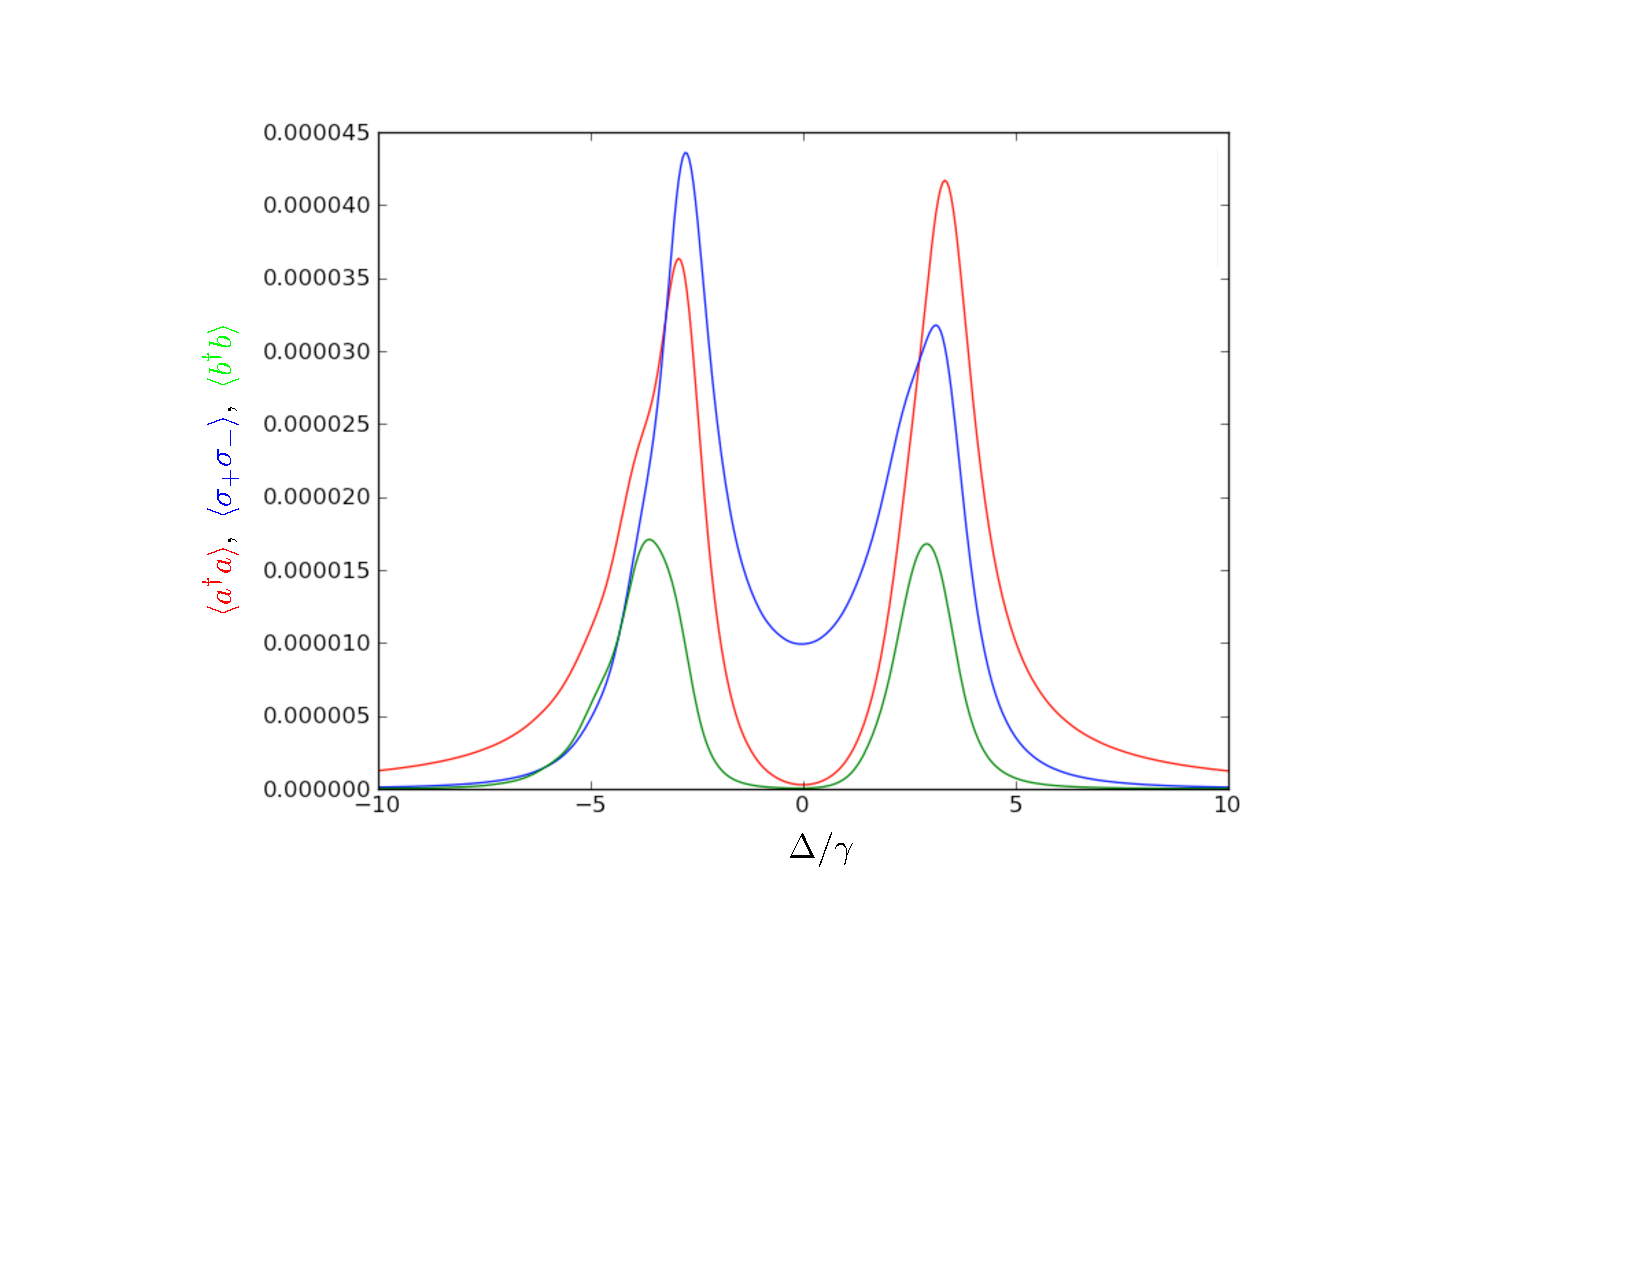
\includegraphics[width=0.474\textwidth]{Figures/5b_gM1}}
\\
\subfloat[\small{$g_M/\gamma = 3$}]{\label{fig5c}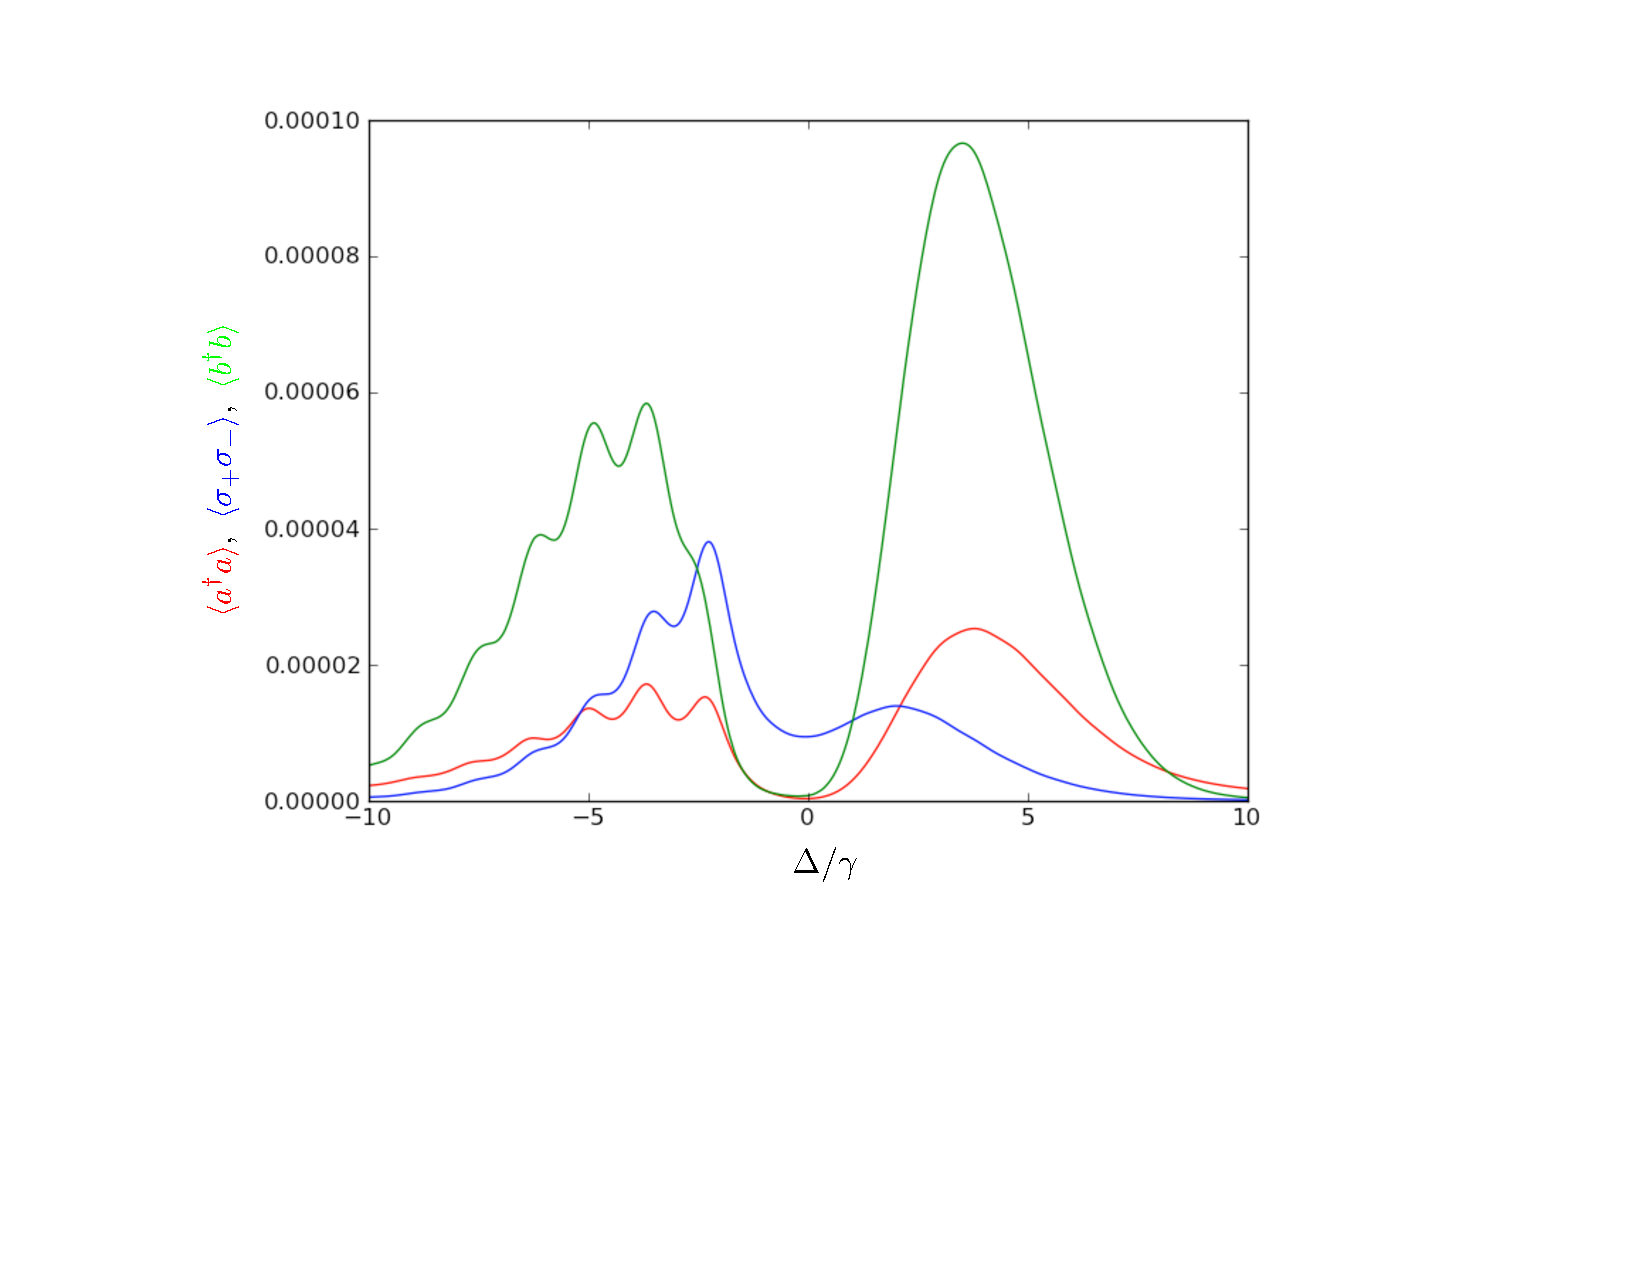
\includegraphics[width=0.474\textwidth]{Figures/5c_gM3}}
\qquad
\subfloat[\small{$g_M/\gamma = 5$}]{\label{fig5d}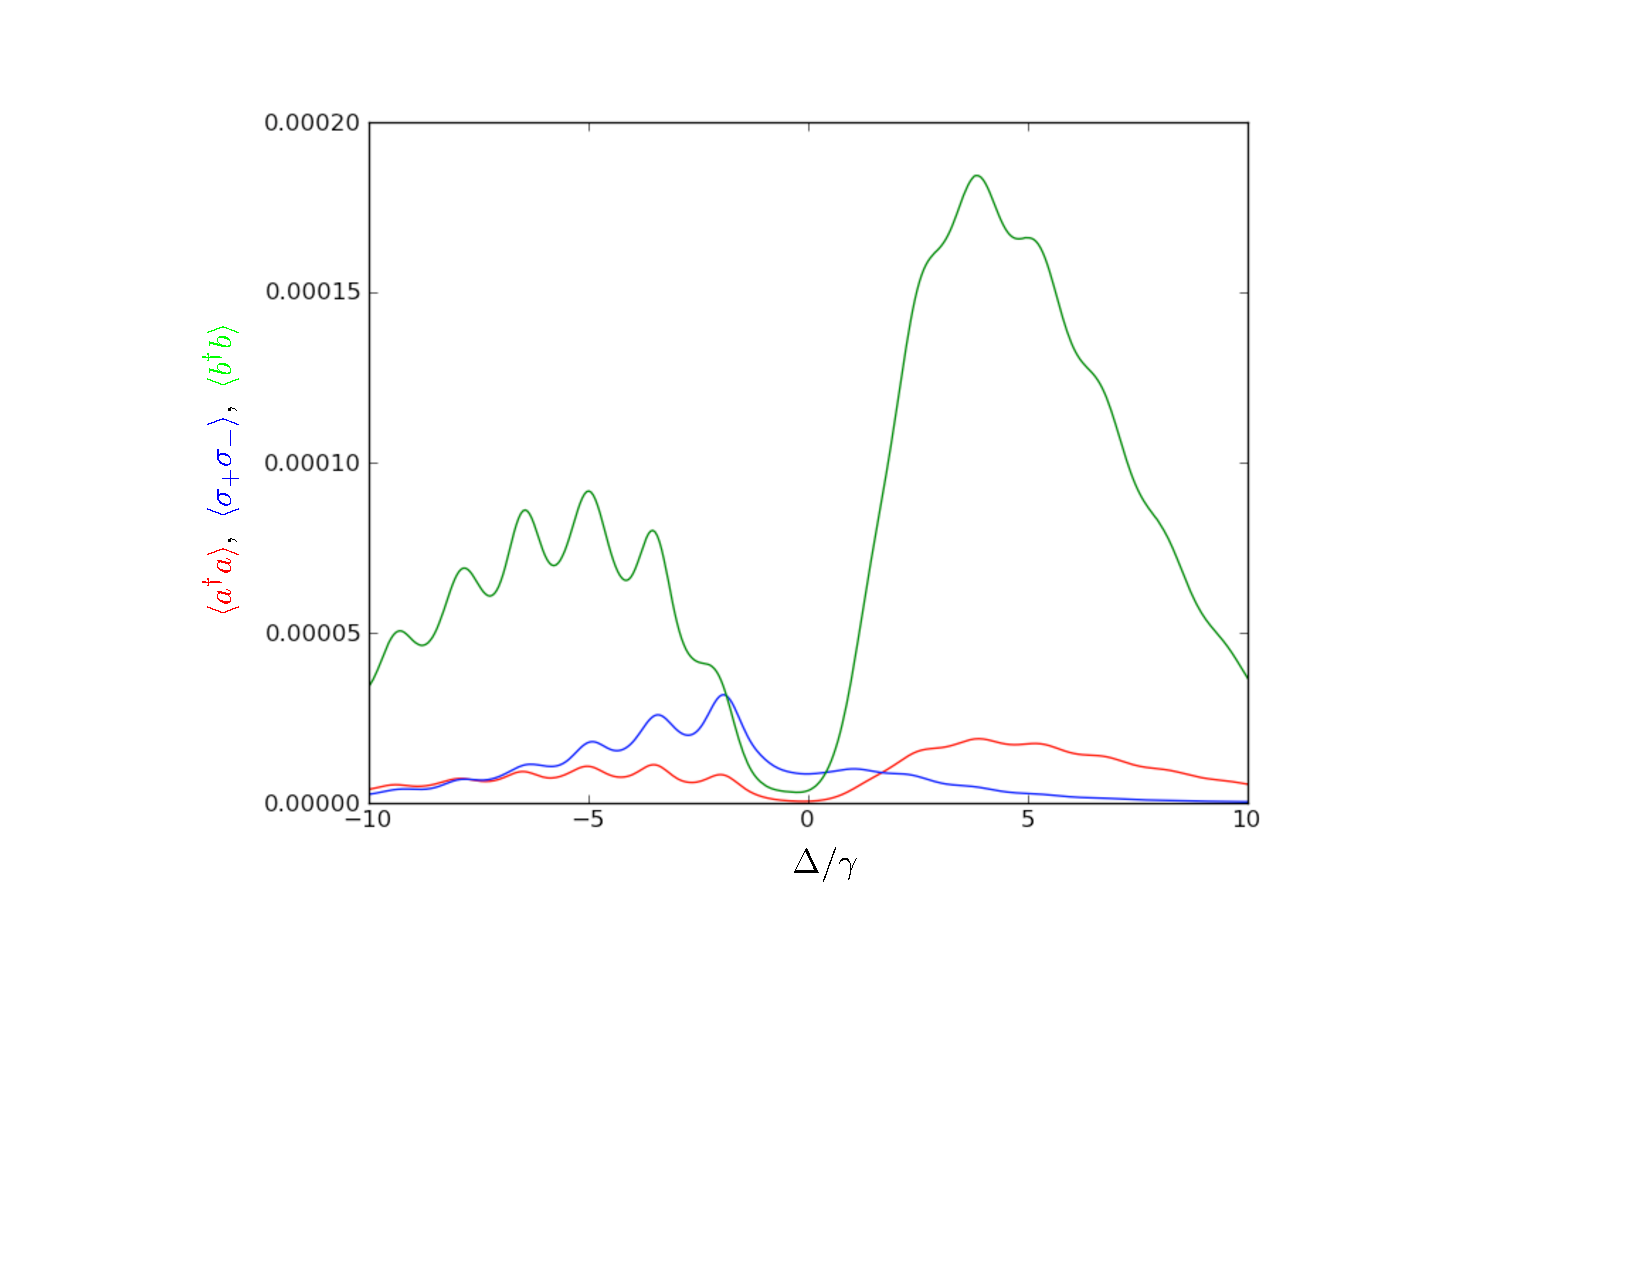
\includegraphics[width=0.474\textwidth]{Figures/5d_gM5}}
\caption[Probe spectra over a range of mechanical coupling rates]{\small{Probe spectra over a range of mechanical coupling rates with set optical coupling. Red traces indicate $\langle \adag a \rangle$, blue traces denote $\langle \splus\sminus \rangle$, and green traces indicate $\langle \bdag b \rangle$. The relevant parameters are $\gamma = \kappa = \omega_M = 1$, $Y/\gamma = 0.01$, and $g/\gamma = 3$. A maximum of 64 phonon excitations is allowed in the oscillator.}}
\label{fig5gM}
\end{figure}

\noindent Finally, we observe that as $g_M$ increases, a larger proportion of the total energy is stored in the form of phonon excitations.

In Fig.~\ref{fig6g}, we present a series of spectra where $g_M$ is constant and we calculate the relevant expectation values over a range of optical coupling values. Considering first Fig.~\ref{fig6a} where $g \ll g_M$, we see any signature of the atom's presence effectively vanishes, and we are in accordance with the cavity-oscillator model of \cite{girvin2011}. Setting $g/\gamma$ equal to unity, the signature vacuum Rabi doublet begins to become evident, but is still somewhat difficult to resolve due to the two peaks lying at $g \simeq \pm 1$. For $g > g_M$, the doublet is completely resolved, and it is clear that their structure is more complex than that of Figs.~\ref{fig5a}-\ref{fig5b}. It follows that as $g$ increases and surpasses $g_M$, a growing amount of the total energy is transferred from the oscillator to the atom-cavity subsystem.

\begin{figure}[htb]
\centering
\subfloat[\small{$g/\gamma = 0.1$}]{\label{fig6a}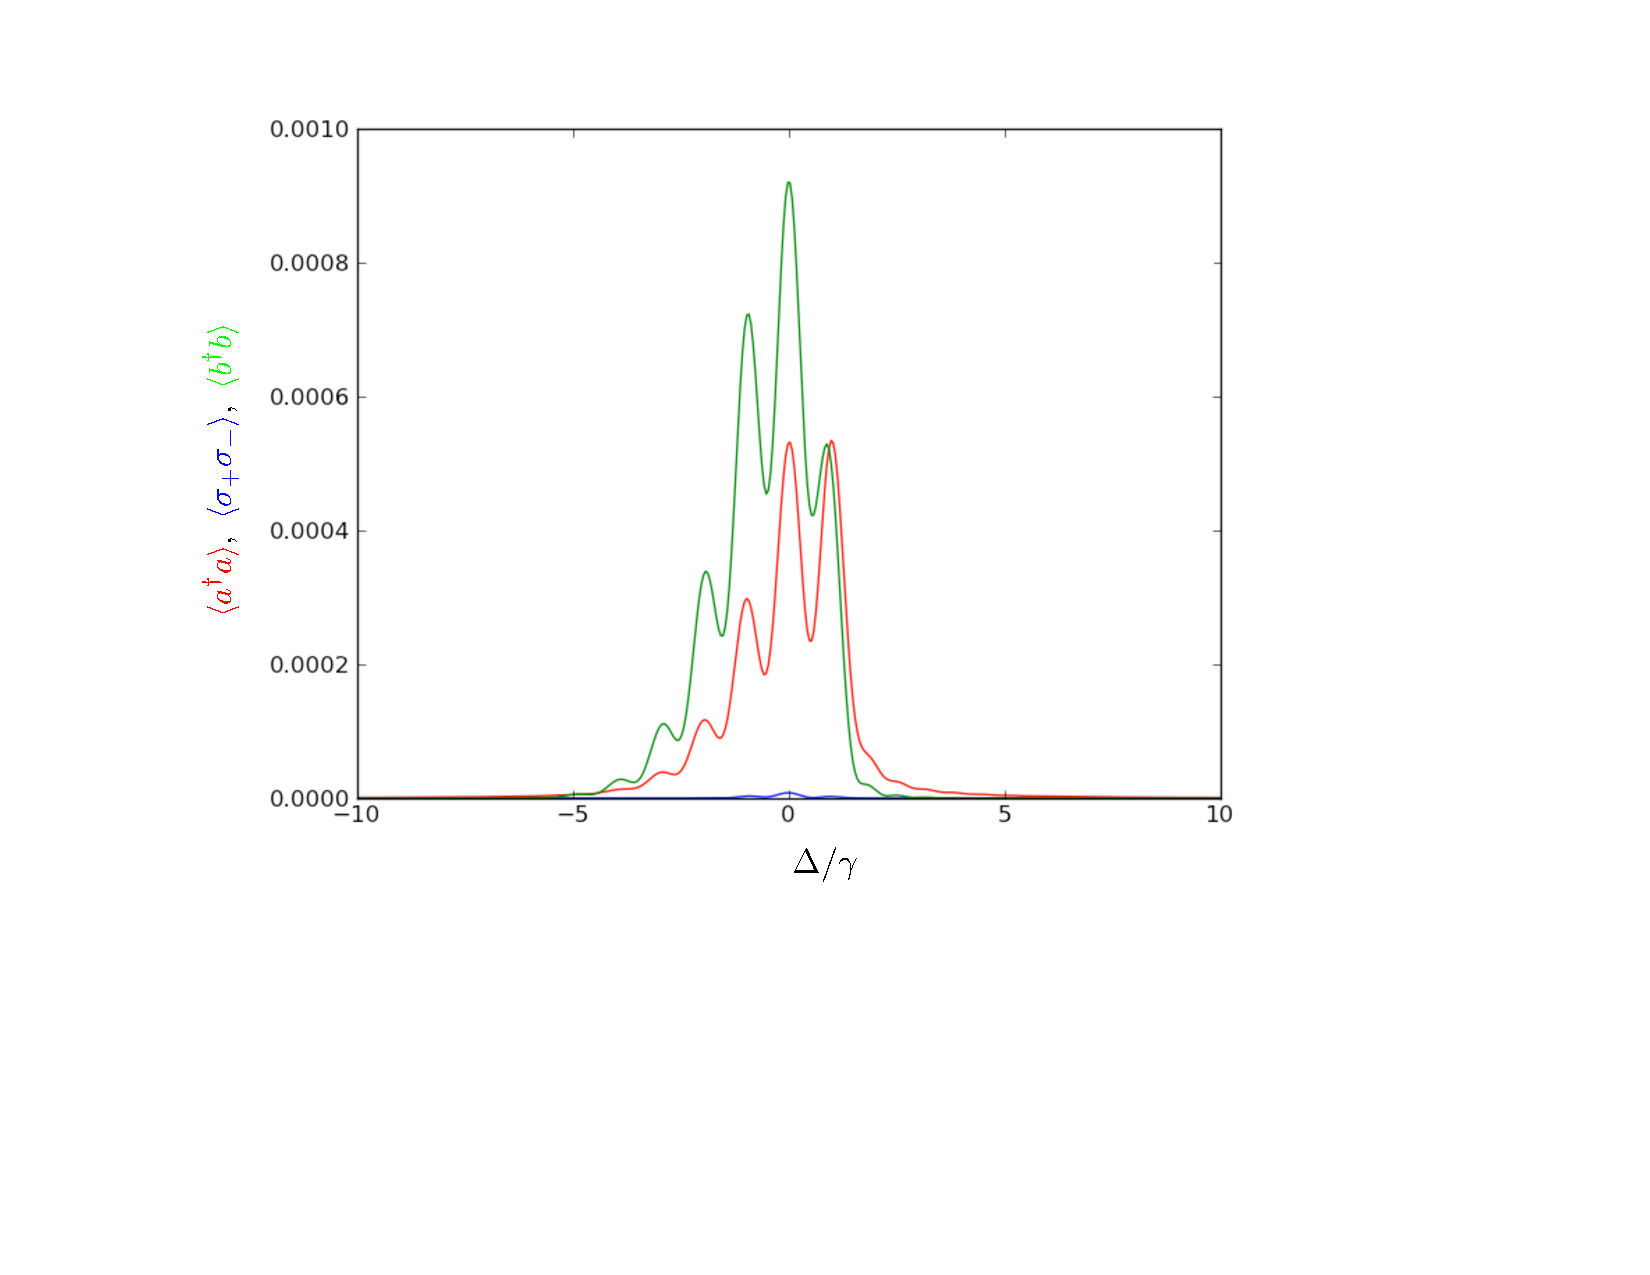
\includegraphics[width=0.474\textwidth]{Figures/6a_g1_10}}
\\
\subfloat[\small{$g/\gamma = 1$}]{\label{fig6b}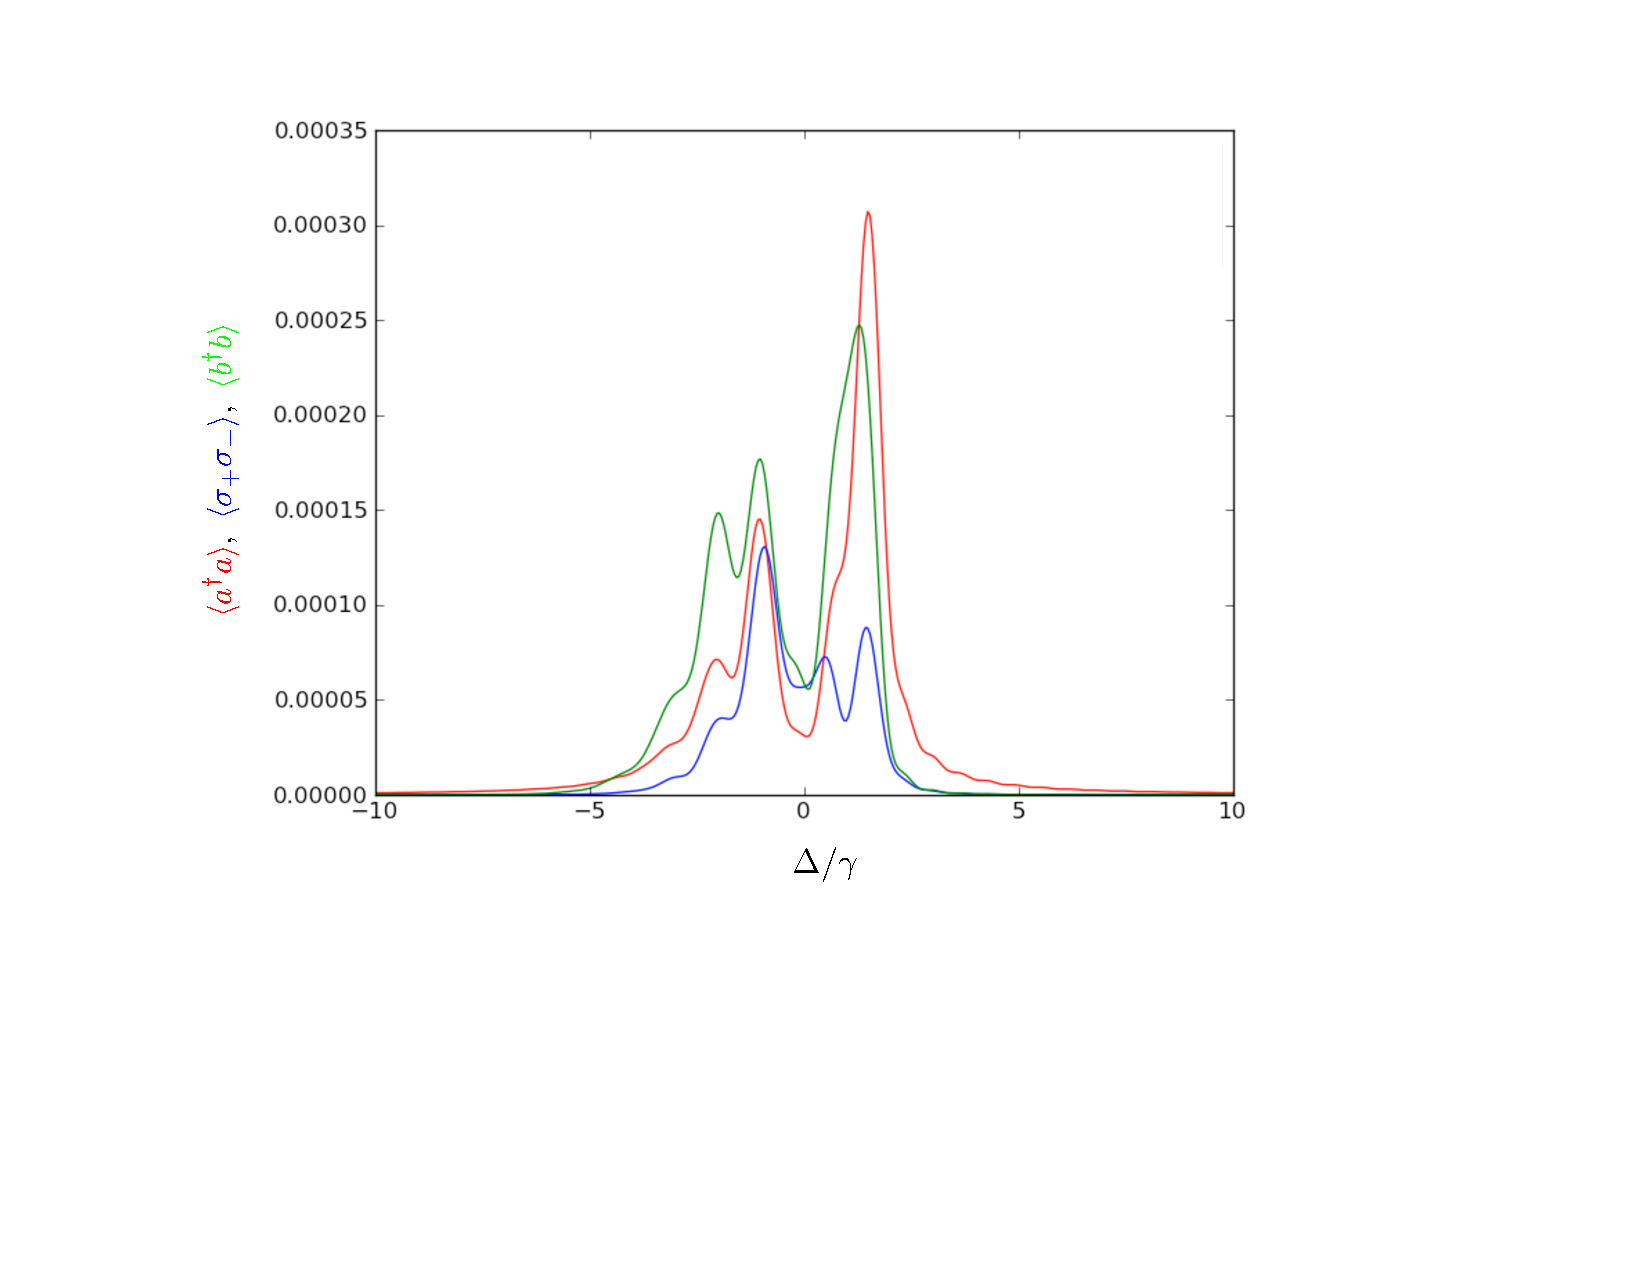
\includegraphics[width=0.474\textwidth]{Figures/6b_g1}}
\qquad
\subfloat[\small{$g/\gamma = 5$}]{\label{fig6c}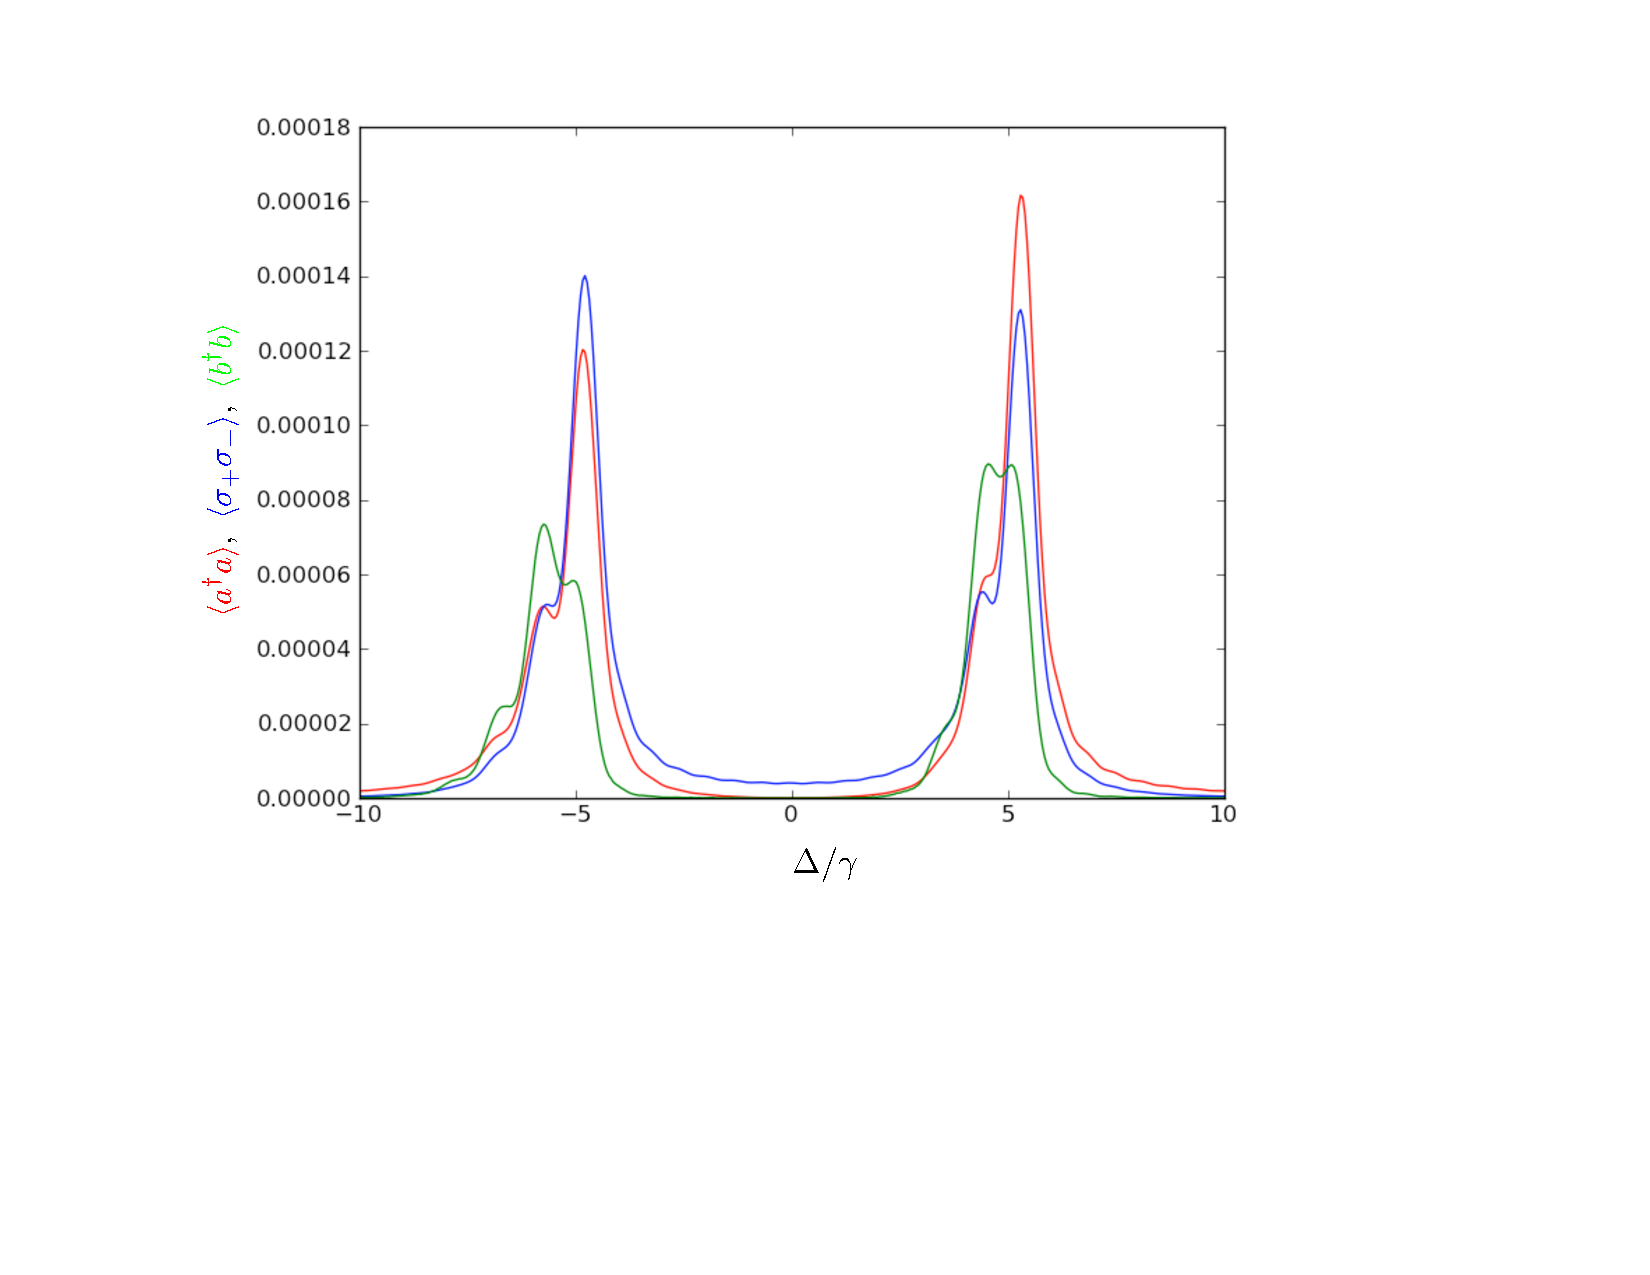
\includegraphics[width=0.474\textwidth]{Figures/6c_g5}}
\caption[Probe spectra over a range of optical coupling rates]{\small{Probe spectra over a range of optical coupling rates with set mechanical coupling. Red traces indicate $\langle \adag a \rangle$, blue traces denote $\langle \splus\sminus \rangle$, and green traces indicate $\langle \bdag b \rangle$. The relevant parameters are $\gamma = \omega_M = g_M = 1$, $\kappa/\gamma = 0.25$, and $Y/\gamma = 0.01$. A maximum of 64 phonon excitations is allowed in the oscillator.}}
\label{fig6g}
\end{figure}

In all of Section 4, on account of the weak incident field, we evaluate each trace with only a single trajectory due to the low probability for a jump to occur. Considering Figs.~\ref{fig5a}-\ref{fig6c}, this approximation is validated, as the highest mean value we see is $\langle \bdag b \rangle \sim 10^{-3}$ in Fig.~\ref{fig6a}, demonstrating that all three subsystems occupy their respective ground states. As a final note, we remark that all values in Figs.~\ref{fig5gM} and \ref{fig6g} are steady-state expectation values, reached after ten spontaneous emission lifetimes.

\section{Photon Statistics}
In the context of cavity QED, photon statistics play a valuable role in many aspects of study. Measurement of the second-order correlation function of a transmitted electromagnetic field allow experimenters to deduce the nonclassical nature of the light source \cite{leach2003}. Indeed, such measurements also provide evidence that certain atomic and cavity quantum states are capable of being ``frozen'' in their time evolution, only to be restarted at a later time as if no such interruption occurred \cite{leach2003}. New types of correlation functions are also being developed, such as $h_{\theta}(\tau)$ by Carmichael \emph{et. al.}, which measures the correlation between a photon detection and conditional field fluctuations, bringing to light the junction between the particle and wave natures of light \cite{leach2003}.

Our investigation of photon statistics begins with consideration of the normalized, steady-state second-order correlation function $g^{(2)}(0)$, specifically the field-field auto-correlation and atom-field cross-correlation. We follow the approach of \cite{brecha1999} in the respective calculations,
%
\begin{align} g^{(2)}_{aa}(0) &= \frac{\evalue{a^{\dag 2} a^2}}{\evalue{\adag a}^2}, \label{eq4.1} \\[5pt]
g^{(2)}_{a\gamma}(0) &= \frac{\evalue{\adag a \, \splus\sminus}}{\evalue{\adag a} \evalue{\splus\sminus}}. \label{eq4.2} \end{align}
%
Typically, $g^{(2)}(0)$ is plotted as a function of parameters such as cavity linewidth $\kappa$ or detuning $\Delta$; in a multiatom ensemble case, the correlation function will be plotted as a function of atomic number \cite{brecha1999}. In the case of cOM, we plot $g^{(2)}(0)$ as a function of mechanical coupling $g_M$. Note that we include mechanical damping with $\kappa_M > 0$, and determine \eqref{eq4.1} and \eqref{eq4.2} on resonance, $\Delta = 0$.

We pause now to justify our choice in Fig.~\ref{fig7g20} for the optical coupling constant $g/\gamma = 1/\sqrt{2}$. Following the approach of \cite{howard1991}, the analytical result for the second-order correlation function at $\tau = 0$ is
%
\be g^{(2)}(0) = 1 + \frac{\Delta\alpha}{\alpha}, \label{eq4.3} \ee
%
where
%
\be \frac{\Delta\alpha}{\alpha} = -2C'_1 \left( \frac{2C}{1 + 2C - 2C'_1} \right), \label{eq4.4} \ee
%
and
%
\be C = \frac{g^2}{\gamma\kappa}, \quad C'_1 = \frac{C}{1 + (\gamma/2\kappa)}. \label{eq4.5} \ee
%
\newpage
\begin{figure}[htb]
\begin{center}
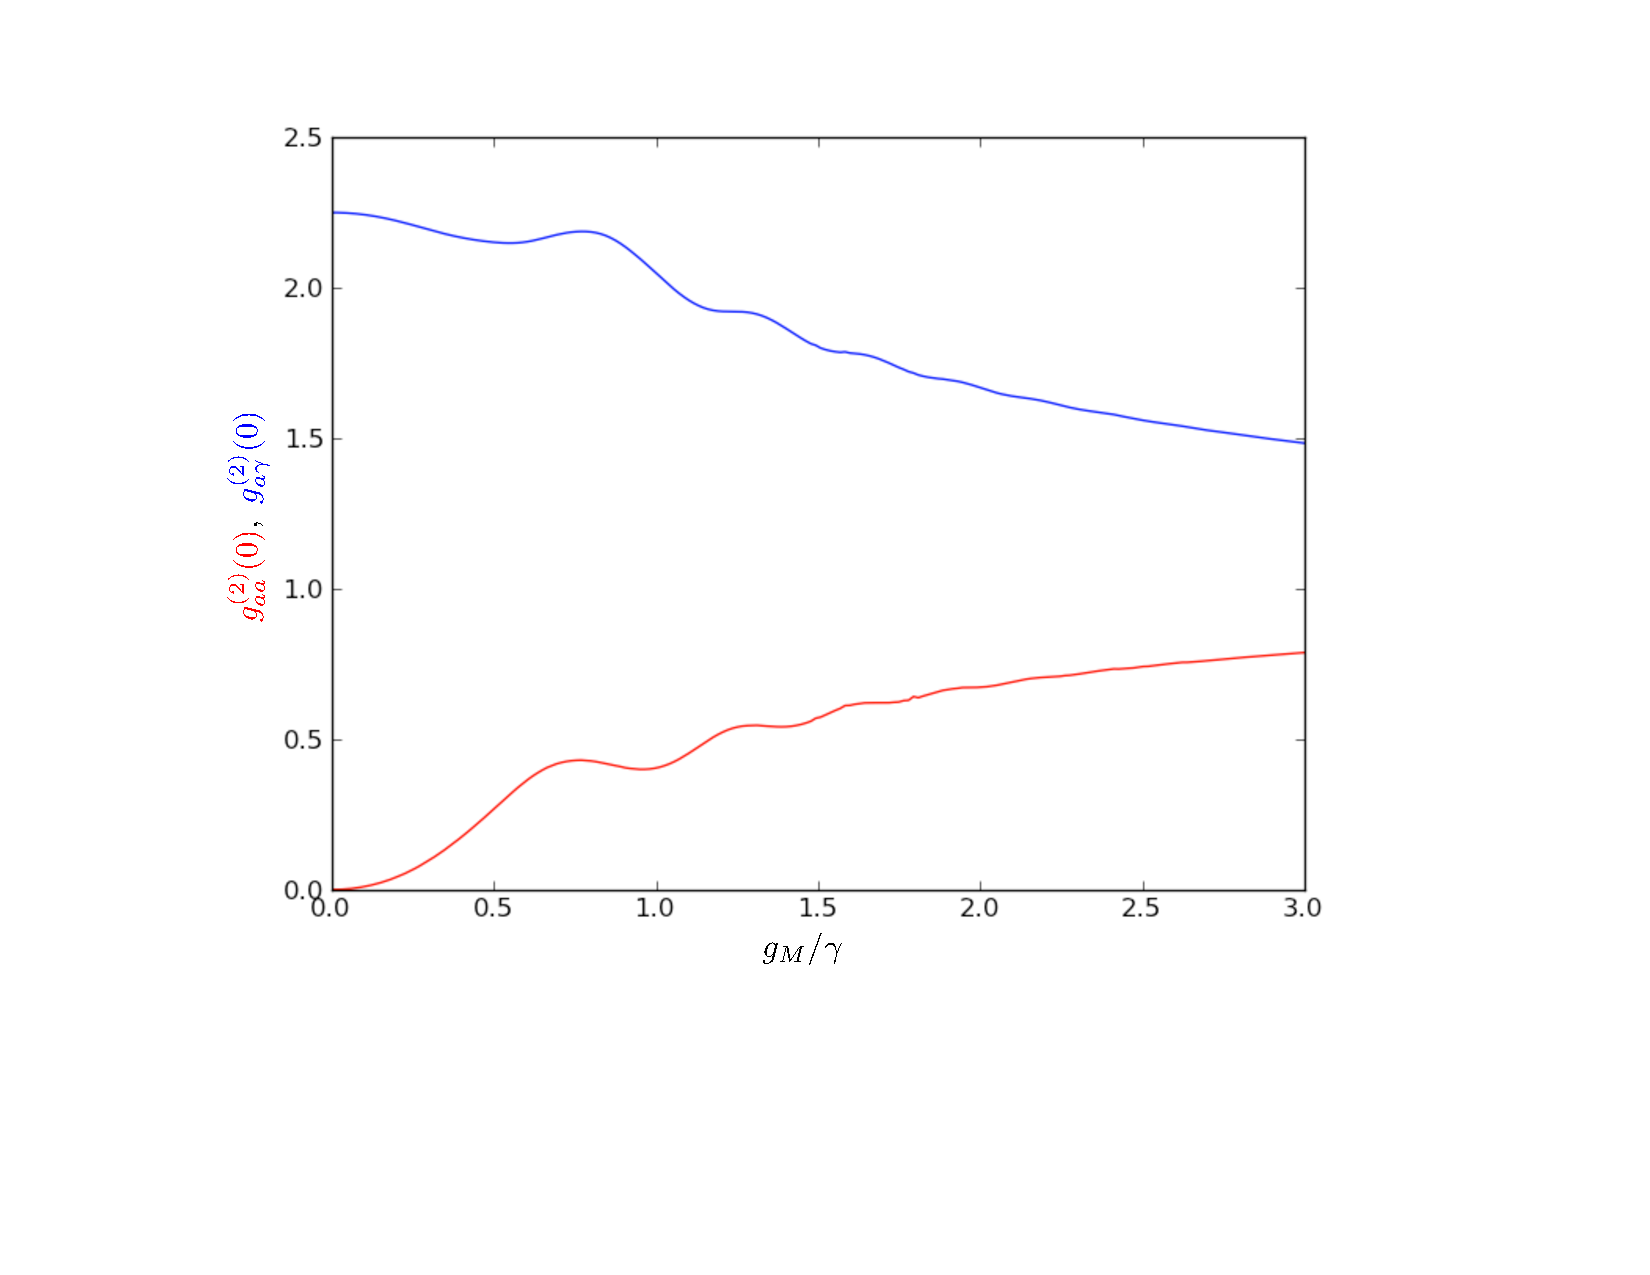
\includegraphics[width=0.85\textwidth]{Figures/7g20}
\caption[A plot of $g^{(2)}(0)$ in the steady state as a function of $g_M$]{\small{A plot of the second-order correlation function $g^{(2)}(0)$, as a function of mechanical coupling $g_M$, after allowing $10\tau_0$ to reach the steady state. The red trace denotes the field-field auto-correlation, while the blue trace indicates the atom-field cross-correlation. The relevant parameters are $\gamma = \omega_M = 1$, $Y/\gamma = 0.01$, $\kappa/\gamma = 0.5$, $g/\gamma = 1/\sqrt{2}$, and $\kappa_M/\gamma = 0.1$. The maximal atom-cavity excitation number is raised to 3, while the phonon excitation limit is raised to 128.}}
\label{fig7g20}
\end{center}
\end{figure}

\noindent The parameter $C$ in \eqref{eq4.5} appears frequently in cQED and is known as the cooperativity. Our objective now is to choose a set of parameters $\left\{ \gamma, \, \kappa, \, g \right\}$ such that the field-field auto-correlation demonstrates perfect photon antibunching, i.e. $g^{(2)}(0) = 0$, in the limit $g_M \to 0$. Using the values $\gamma = 1$ and $\kappa = \gamma/2 = 0.5$, we see from \eqref{eq4.5} that $C'_1 = C/2$ such that \eqref{eq4.4} reduces to
%
\be \frac{\Delta\alpha}{\alpha} = -C \left( \frac{2C}{1 + C} \right), \label{eq4.6} \ee
%
and because $C = 2g^2$ we find
%
\be \frac{\Delta\alpha}{\alpha} = -2g^2 \left( \frac{4g^2}{1 + 2g^2} \right) = -1, \label{eq4.7} \ee
%
where the value of $-1$ is chosen in order to satisfy $g^{(2)}(0) = 0$ in \eqref{eq4.3}. We obtain from \eqref{eq4.7}
%
\be -8g^4 + 2g^2 + 1 = 0, \label{eq4.8} \ee
%
a quadratic equation in $g^2$; defining $x \equiv g^2$ and using the quadratic formula we obtain $x = (1/8) \pm (3/8)$. The negative root of $x$ is discarded as it ultimately yields an unphysical (imaginary) value for $g$. The optimal value for the coupling constant must then be $g_{\text{opt}} = \sqrt{x} = \sqrt{1/2}$, validating our choice in Fig.~\ref{fig7g20}.

We observe in the traces of $g^{(2)}(0)$ that the field-field and atom-field correlations are respectively antibunched and bunched without any optomechanical coupling present. As the oscillator coupling is increased, both correlations approach a value of unity, indicating they come closer to obeying Poissonian photon statistics. This is a similar result to the influence of parameters $N$ (atom number) and $\Delta$ on the correlations in \cite{brecha1999}.

Continuing with our discussion of photon statistics, we generalize to a calculation of the time-varying, normalized, second-order correlation function $g^{(2)}(\tau)$. We again calculate the field-field auto-correlation and atom-field cross-correlation, plus we add the oscillator-field cross-correlation. Rather than referring to mathematical formalism as with $g^{(2)}(0)$, we numerically evaluate the former function, again using the technique of quantum trajectories and the \texttt{mcsolve} function of QuTiP.

We see from Figs.~\ref{fig8a} and \ref{fig8b} that the field-field and atom-field correlations undergo identical time evolution, starting in a bunched state and then oscillating anharmonically about unity. The oscillator-field correlations begin in a highly bunched state, $g^{(2)}(\tau) \gg 1$, and within a time period of $5\tau_0$ have decayed and oscillate about unity. Both statements are somewhat similar to the results of \cite{brecha1999}.

In order to calculate the $g^{(2)}(\tau)$, we first allow the initial ground state $\ket{\psi(0)}$ to evolve in time for $20\tau_0$ under the Hamiltonian of \eqref{eq2.107}, with $\Delta = 0$, to the steady state $\ket{\psi(20\tau_0)}_{ss}$. One of the three possible jump operators is then applied to the latter steady state, and the associated expectation value after another $20\tau_0$ due to the final state is used to determine the respective correlation functions. Finally, in order to normalize, the value is divided by the steady-state mean photon number under $\ket{\psi(20\tau_0)}_{ss}$ for each time step. To better illustrate the process, we denote the three final states after a jump and reaching the steady state as
%
\be \ket{\psi_a}_{ss} = \hat{\Upsilon}_{20} \, a \ket{\psi(20\tau_0)}_{ss}, \quad \ket{\psi_{\gamma}}_{ss} = \hat{\Upsilon}_{20} \, \sminus \ket{\psi(20\tau_0)}_{ss}, \quad \ket{\psi_b}_{ss} = \hat{\Upsilon}_{20} \, b \ket{\psi(20\tau_0)}_{ss}, \label{eq4.9} \ee
%
\newpage
\begin{figure}[htb]
\centering
\subfloat[\small{field-field}]{\label{fig8a}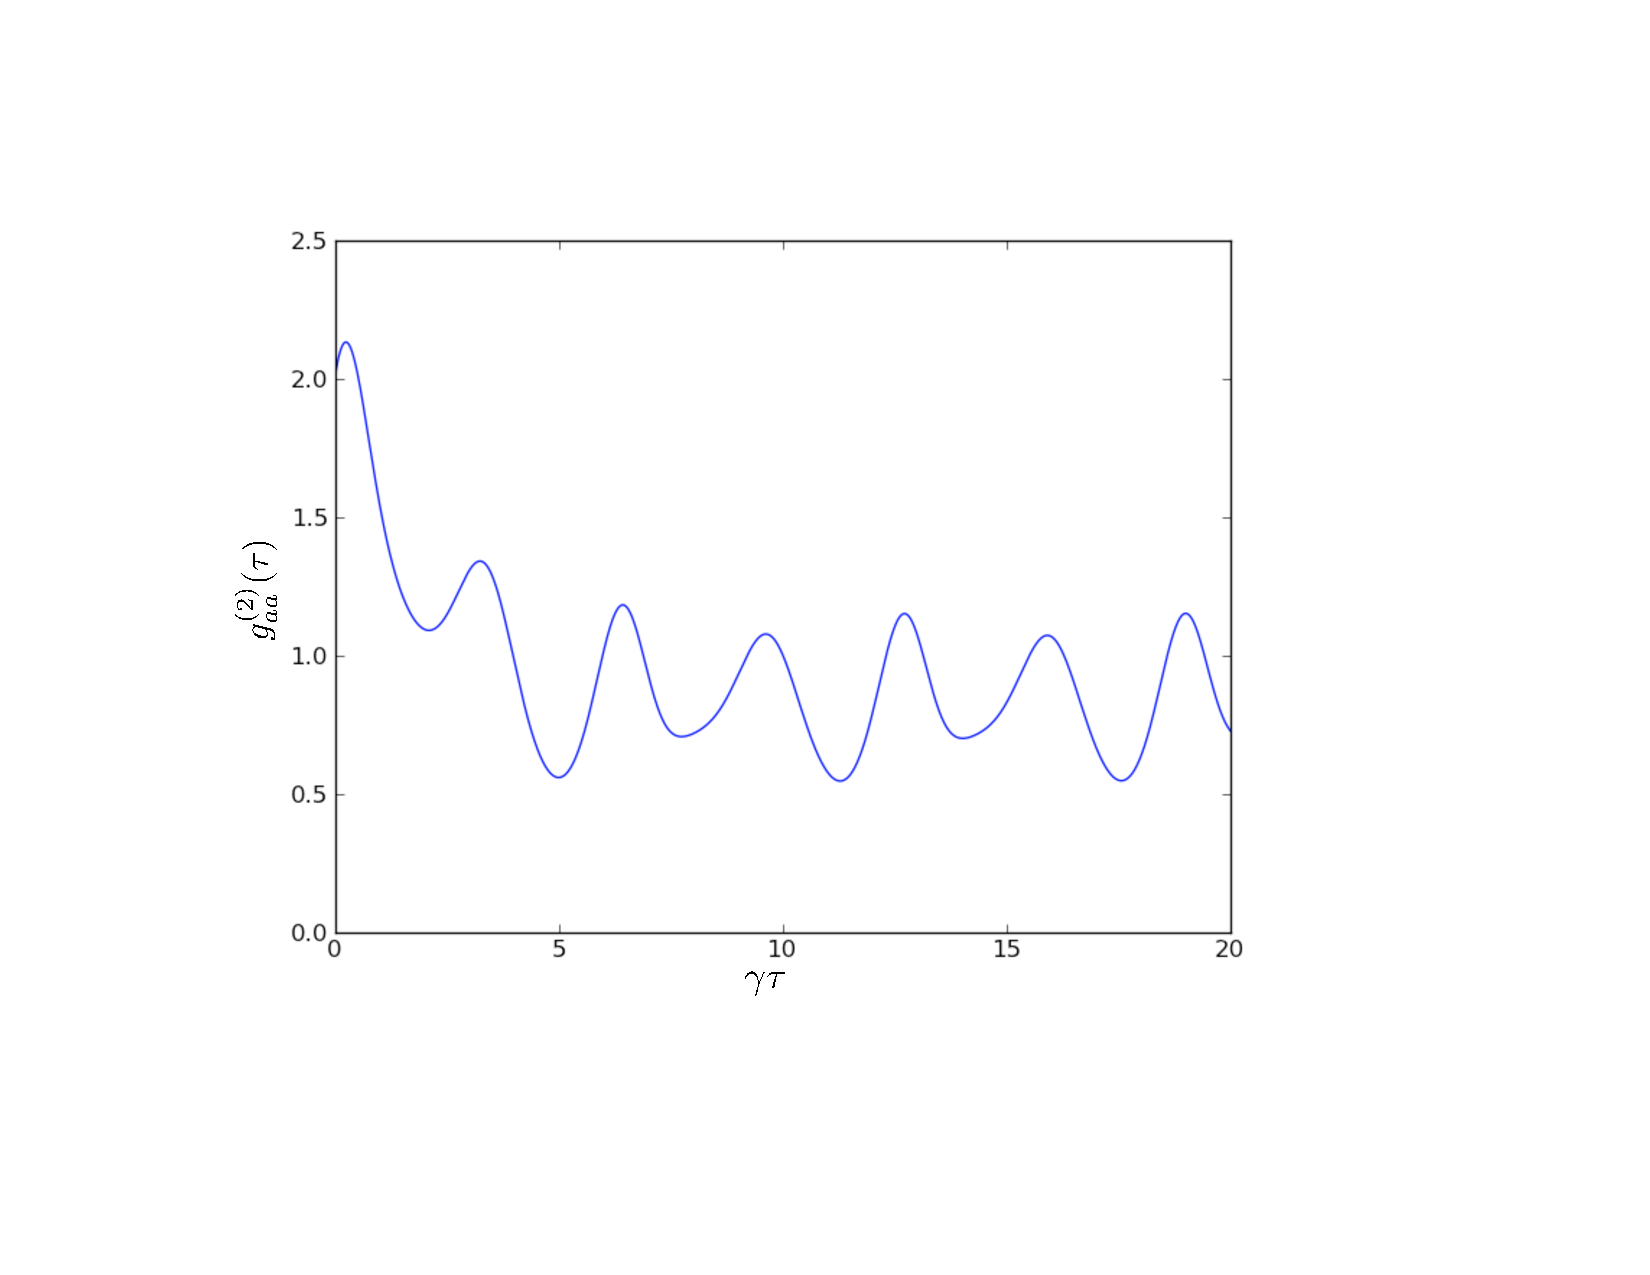
\includegraphics[width=0.474\textwidth]{Figures/8a_g2aatau}}
\qquad
\subfloat[\small{atom-field}]{\label{fig8b}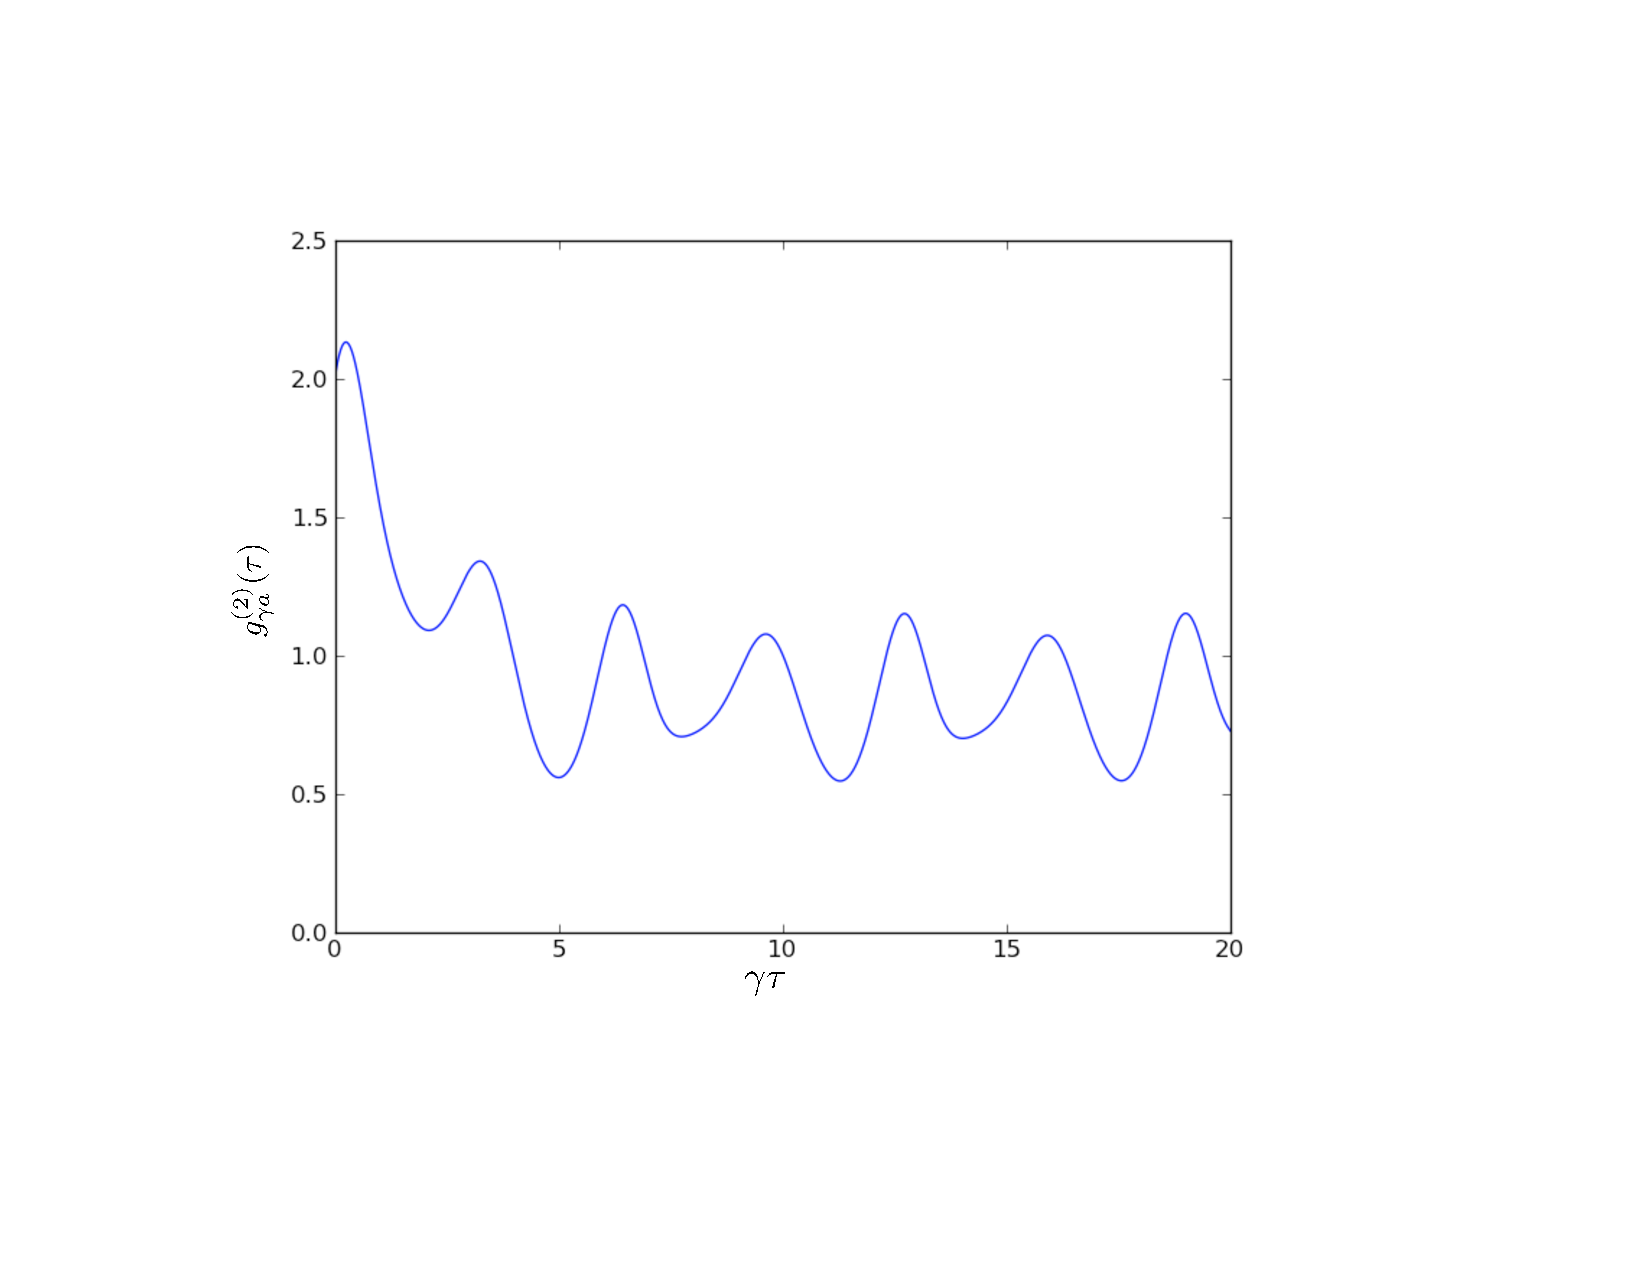
\includegraphics[width=0.474\textwidth]{Figures/8b_g2gatau}}
\\
\subfloat[\small{oscillator-field}]{\label{fig8c}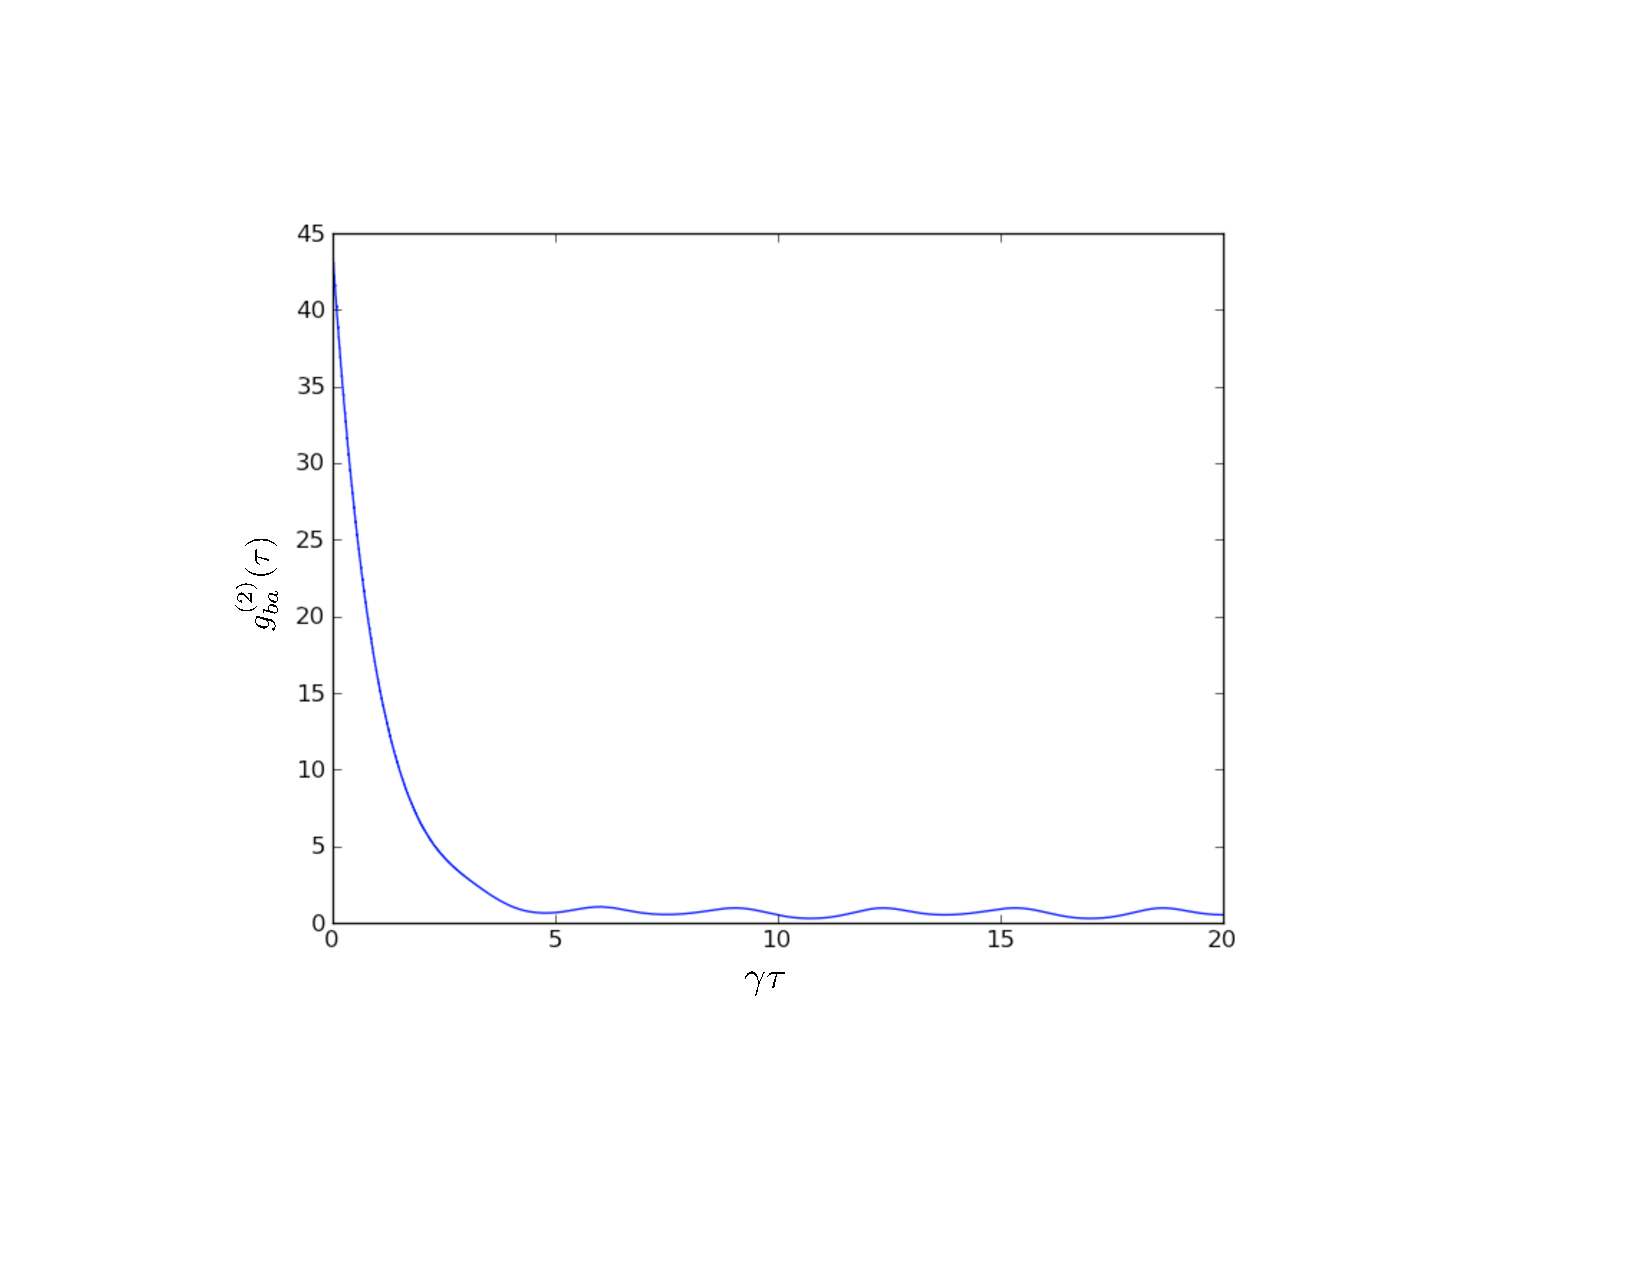
\includegraphics[width=0.474\textwidth]{Figures/8c_g2batau}}
\caption[Plots of $g^{(2)}(\tau)$ ]{\small{Plots of $g^{(2)}(\tau)$ over time. All steady-state expectation values are determined after $20\tau_0$. The relevant parameters are $\gamma = \omega_M = g_M = 1$, $\kappa/\gamma = 0.5$, $g/\gamma = 1/\sqrt{2}$, $\kappa_M/\gamma = 0.1$, and $Y/\gamma = 0.01$. As in Fig.~\ref{fig7g20}, we allow a maximum of 3 photon and 128 phonon excitations.}}
\label{fig8g2tau}
\end{figure}

\noindent where $\hat{\Upsilon}_{20}$ is an operator denoting another period of $20\tau_0$ of free evolution under the resonant $H$. The three correlation functions are then calculated by
%
\begin{align} g^{(2)}_{aa}(\tau) &= \frac{\langle \adag a \rangle_{a,ss}}{\langle \adag a \rangle_{ss}}, \label{eq4.10} \\[5pt]
g^{(2)}_{\gamma a}(\tau) &= \frac{\langle \splus\sminus \rangle_{\gamma,ss}}{\langle \adag a \rangle_{ss}}, \label{eq4.11} \\[5pt]
g^{(2)}_{ba}(\tau) &= \frac{\langle \bdag b \rangle_{b,ss}}{\langle \adag a \rangle_{ss}}. \label{eq4.12} \end{align}
%
Again for clarification, we note that the numerators of \eqref{eq4.10}-\eqref{eq4.12} are calculated using the respective states of \eqref{eq4.9}, while all three denominators are determined using $\ket{\psi(20\tau_0)}_{ss}$. The results of Fig.~\ref{fig8g2tau} show a clear deviation from the non-optomechanical case as seen in \cite{brecha1999}.
\chapter{Conclusion}
In this thesis, we have investigated the probe spectra and nonclassical photon statistics of a damped, weakly-driven cavity optomechanical system. In order to best understand such results, three principle theoretical techniques are introduced, and a more straightforward classical oscillator in two different initial states is examined. A full quantum treatment calculates the probe spectra under various values for both the optical and mechanical coupling rates, as well as determining second-order correlation functions for the field-field auto-correlation, atom-field, and oscillator-field cross-correlations.

\section{Summary}
In Chapter 2, we illustrate three crucial theoretical frameworks necessary to conduct an investigation of our cOM system. The master equation in Lindblad form is derived in order to describe the dynamics of an open quantum system, and we utilize a system-reservoir approach in the interaction picture, as well as the Born-Markov approximation and some time-dependent perturbation theory, to arrive at the final result. In addition, consideration of the system at zero temperature is shown to further simplify the master equation and instructs our approach to the inclusion of damping terms.

The theory of quantum trajectories is introduced, a way to model a cQED experiment as a scattering interaction and reduce the number of system variables to be monitored from an effectively infinite number to manageable finite quantity. The idea of a measurement record is described, where a record of a given time interval and the various quantum jumps are monitored, and the state of the system is conditioned upon the record obtained. The density operator is written in the basis of measurement records, both with and without known initial states. Trajectories and the master equation are integrated using superoperator formalism, where the latter is comprised of two pieces respectively describing between-jump evolution and the jumps themselves. As a final note on trajectories, the dynamics of pure states are considered in the presence of dissipation, enabling us to write the appropriate jump operator, to understand that an initial pure also ends as a pure state, and to determine the probability for records with and without a jump detected.

Lastly, chapter 2 describes the formalism of, and some contrasts with cQED to, cavity optomechanics. The position operator of the mechanical oscillator, a spring-mounted end mirror of the optical cavity, is written using phonon creation and annihilation operators, and the standard linear optomechanical coupling Hamiltonian is written. The optomechanical coupling rate is itself related to the oscillator in terms of its mass, resonant frequency, and frequency modulation of the cavity mode based on distance from equilibrium. Expectations for the output of the probe spectra are briefly noted from previous work, and the full optomechanical Hamiltonian is written.

Chapter 3 considers a classical mechanical oscillator in the scenarios of (i) sinusoidal and (ii) thermal or Brownian fluctuations. The position operator of the oscillator is cast in classical terms, and expectation values are calculated to their steady state conditions, requiring at least ten atomic spontaneous emission lifetimes. We also justify our choices of parameter values, pointing out experimental precedent.

Chapter 4 brings a fully quantum mechanical treatment of the cOM system, first in the form of the calculation and plotting of various probe spectra. Three principle expectation values are determined in the steady state over a range of incident field detunings, varying first the optomechanical coupling and then the optical Jaynes-Cummings coupling rates. Variation from the expected vacuum Rabi splitting is explored, especially due to the relationship of the two coupling rates. The role of photon statistics in cQED is briefly introduced, followed by calculation and plotting of $g^{(2)}(0)$ for both auto- and cross-correlations within the atom-field subsystem. Finally, the time-dependent correlation $g^{(2)}(\tau)$ is calculated, with an explanation of the process involved in doing so, which shows evidence of anharmonicity.

\section{Future Work}
A few avenues of future investigation into this cavity optomechanical system become apparent in this thesis, first of which is the optomechanical Hamiltonian itself. While we consider the standard linear coupling, other configurations are possible such as quadratic coupling \cite{li2012, agarwal2011}. Such a change would require a recalculation of all probe spectra and correlation functions in order to determine the effect. The coupling parameters may be varied over larger intervals in finer steps in order to study their signature on the system, especially through the probe spectra. The effect of temperature on the movable end mirror, as well as the oscillator linewidth $\kappa_M$, is also left mostly unexplored. Similarly, it seems prudent to consider larger number of phonon excitations in calculating the various correlation functions. When examining the latter, additional functions could be calculated such as additional auto- and cross-correlations involving the atom and oscillator. Lastly, deeper study into the physical processes of the system will be required in order to explain the features of the many plots in Chapter 4, namely the peaks of the probe spectra and various oscillatory behaviors of the correlation functions.

\appendix
\chapter{Classical Oscillator Code}
We show the code in QuTiP to generate Figs.~\ref{fig3Harmonic} and \ref{fig4Thermal}.

\begin{verbatim}
import math
import pylab as pl
from qutip import *

# system parameters
n = 2 # photon excitations
gamma = 1
kappa = 1
Y = 0.01
g = 3
g_M = 2
beta = 1
beta_star = 1

# initial state
psi0 = tensor(fock(2,1), fock(n,0))

# operators of interest
sm = tensor(sigmam(), qeye(n))
a = tensor(qeye(2), destroy(n))

# collapse operators
collapse = [sqrt(2*kappa)*a, sqrt(gamma)*sm]

# expectation values
evalue_list = [a.dag()*a, sm.dag()*sm]

# timescale
harmonic_time = linspace(0,15,7500)
thermal_time = linspace(0,10,6000)

# build the time-dependent Hamiltonian
def H_t(t, args):
    H0 = args[0]
    H1 = args[1]
    omega_M = args[2]

    return H0 + H1 * sin(omega_M*t)

H0 = Y*(a + a.dag()) + g*(a*sm.dag() + a.dag()*sm)
H1 = g_M*a.dag()*a
omega_M = 1

H_args = (H0, H1, omega_M)

# evaluate the expectation values
evalues = odesolve(H_t, psi0, harmonic_time, collapse, evalue_list, H_args)

# write to data file
import csv
filename1 = 'harmonic_oscillator.csv'
with open(filename1, 'wb') as f:
    writer = csv.writer(f)
    writer.writerows(array([harmonic_time, evalues[0], evalues[1]]).transpose())
    
# generate a pseudorandom value for the thermal state
xi = random.random()

# define a new Hamiltonian
H_therm = Y*(a + a.dag()) + g*(a*sm.dag() + a.dag()*sm) + xi*g_M*a.dag()*a

# evaluate the expectation values a second time
evalues_therm = odesolve(H_therm, psi0, thermal_time, collapse, evalue_list)

# write to data file
filename2 = 'thermal_oscillator.csv'
with open(filename2, 'wb') as f:
    writer = csv.writer(f)
    writer.writerows(array([thermal_time, evalues_therm[0], 
    	evalues_therm[1]]).transpose())

# plot the graphs to verify
pl.plot(harmonic_time, evalues[0], 'r', harmonic_time, evalues[1], 'b')
pl.xlabel('gamma*t')
pl.ylabel('expectation value')
pl.legend(('cavity', 'atom'))
pl.show()

pl.plot(thermal_time, evalues_therm[0], 'r', thermal_time, evalues_therm[1], 'b')
pl.xlabel('gamma*t')
pl.ylabel('expectation value')
pl.legend(('cavity', 'atom'))
pl.show()
\end{verbatim}
\chapter{Probe Spectrum Code}
We show the code in QuTiP to generate Fig.~\ref{fig5d}.

\begin{verbatim}
import math
import pylab as pl
from qutip import *

# system parameters
n = 2
m = 64
gamma = 1
kappa = 1
Y = 0.01
g = 3
g_M = 5
omega_M = 1
kappa_M = 0
ntraj = 1

# initial state
psi0 = tensor(fock(2,1), fock(n,0), fock(m,0))

# operators
sig_plus = tensor(sigmap(), qeye(n), qeye(m))
a = tensor(qeye(2), destroy(n), qeye(m))
b = tensor(qeye(2), qeye(n), destroy(m))

# collapse operators
collapse = [sqrt(2*kappa)*a, sqrt(gamma)*sig_plus.dag()]

# expectation values
evalue_list = [a.dag()*a, sig_plus*sig_plus.dag(), b.dag()*b]

# lists of steady-state values
adaga_list = []
spsm_list = []
bdagb_list = []

Delta_list = linspace(-10,10,400)
times_list = linspace(0,10,1000)

# build the probe spectrum
for Delta in Delta_list:
    H = Delta*a.dag()*a + Delta*sig_plus*sig_plus.dag() + omega_M*b.dag()*b 
    	+ Y*(a + a.dag()) + g*((a*sig_plus) + (a.dag()*sig_plus.dag())) 
	+ g_M*a.dag()*a*(b + b.dag())
    evalues = mcsolve(H, psi0, times_list, ntraj, collapse, evalue_list)
    adaga_list.append(evalues[0][-1])
    spsm_list.append(evalues[1][-1])
    bdagb_list.append(evalues[2][-1])

# plot the probe spectrum
pl.plot(Delta_list, adaga_list, 'r', Delta_list, spsm_list, 'b', 
	Delta_list, bdagb_list, 'g')
pl.xlabel('detuning')
pl.ylabel('steady-state values')
pl.legend(('cavity', 'atom', 'oscillator'))
pl.show()
\end{verbatim}
\chapter{Correlation Function Code I}
We show the code in QuTiP to generate Fig.~\ref{fig7g20}.

\begin{verbatim}
import math
import pylab as pl
from qutip import *

# system parameters
n = 3
m = 128
gamma = 1
kappa = 0.5
Y = 0.01
g = 1/sqrt(2.0)
omega_M = 1
kappa_M = 0.1
ntraj = 1

# initial state
psi0 = tensor(fock(2,1), fock(n,0), fock(m,0))

# operators
sig_plus = tensor(sigmap(), qeye(n), qeye(m))
a = tensor(qeye(2), destroy(n), qeye(m))
b = tensor(qeye(2), qeye(n), destroy(m))

# collapse operators
collapse = [sqrt(2*kappa)*a, sqrt(gamma)*sig_plus.dag(), sqrt(kappa_M)*b]

# expectation values
evalue_list = [a.dag()*a.dag()*a*a, a.dag()*a*sig_plus*sig_plus.dag(), a.dag()*a,
 sig_plus*sig_plus.dag()]

# lists of steady-state values
fieldfield_list = []
atomfield_list = []

times_list = linspace(0,20,2000)
gM_list = linspace(0,3,200)

# build the correlation plots
for g_M in gM_list:
    H = omega_M*b.dag()*b + Y*(a + a.dag()) 
    + g*((a*sig_plus) + (a.dag()*sig_plus.dag())) + g_M*a.dag()*a*(b + b.dag())
    evalues = mcsolve(H, psi0, times_list, ntraj, collapse, evalue_list)
    fieldfield_list.append(evalues[0][-1]/(evalues[2][-1]**2))
    atomfield_list.append(evalues[1][-1]/(evalues[2][-1]*evalues[3][-1]))

# plot the correlation functions
pl.plot(gM_list, fieldfield_list, 'r', gM_list, atomfield_list, 'b')
pl.xlabel('g_M')
pl.ylabel('intensity correlation values')
pl.legend(('field-field', 'atom-field'))
pl.show()
\end{verbatim}
\chapter{Correlation Function Code II}
We show the code in QuTiP to generate Fig.~\ref{fig8g2tau}.

\begin{verbatim}
import math
import pylab as pl
from qutip import *

# system parameters
n = 3
m = 128
gamma = 1
kappa = 0.5
Y = 0.01
g = 1/sqrt(2.0)
g_M = 1
omega_M = 1
kappa_M = 0.1
ntraj = 1

# initial state
psi0 = tensor(fock(2,1), fock(n,0), fock(m,0))

# operators
sm = tensor(sigmam(), qeye(n), qeye(m))
a = tensor(qeye(2), destroy(n), qeye(m))
b = tensor(qeye(2), qeye(n), destroy(m))

# collapse operators
collapse = [sqrt(2*kappa)*a, sqrt(gamma)*sm]

# expectation values
evalue_list = [a.dag()*a, sm.dag()*sm, b.dag()*b]

# find the expectation values
times_list = linspace(0,20,4000)

H = omega_M*b.dag()*b + Y*(a + a.dag()) + g*((a*sm.dag()) + (a.dag()*sm)) 
+ g_M*a.dag()*a*(b + b.dag())

evalues = mcsolve(H, psi0, times_list, ntraj, collapse, evalue_list)

# determine second initial state
next_state = mcsolve(H, psi0, times_list, ntraj, collapse, [])
psi_ss = next_state[0][-1]

psi1 = a*psi_ss
psi2 = sm*psi_ss
psi3 = b*psi_ss

# calculate correlations for g(2)aa
evalues_a = mcsolve(H, psi1, times_list, ntraj, collapse, evalue_list)

counter_max = len(times_list)

g2_aa_list = []

for tau in arange(counter_max):
    g2_aa_list.append(evalues_a[0][tau]/evalues[0][-1])

# calculate correlations for g(2)ga
evalues_g = mcsolve(H, psi2, times_list, ntraj, collapse, evalue_list)

g2_ga_list = []

for tau in arange(counter_max):
    g2_ga_list.append(evalues_g[0][tau]/evalues[0][-1])

# calculate correlations for g(2)ba
evalues_b = mcsolve(H, psi3, times_list, ntraj, collapse, evalue_list)

g2_ba_list = []

for tau in arange(counter_max):
    g2_ba_list.append(evalues_b[0][tau]/evalues[0][-1])

# plot the correlation functions
pl.plot(times_list, g2_aa_list)
pl.show()

pl.plot(times_list, g2_ga_list)
pl.show()

pl.plot(times_list, g2_ba_list)
pl.show()
\end{verbatim}

\backmatter

\bibliographystyle{unsrt}
\addcontentsline{toc}{chapter}{References}
\bibliography{Thesis}
\end{document}